\documentclass[12pt, twoside, openright, thesis]{settings/chthes}

%% ============================================================
%%  Packages
%% ============================================================
\usepackage{xltabular}
\usepackage{natbib}
\usepackage{nomencl}
\usepackage[quotchapII]{settings/fncystyle}
\usepackage{makecell}
\usepackage{setspace}
\usepackage{graphics}
\usepackage{graphicx}
\usepackage{tabularx}
\usepackage{lscape}
\setcounter{MaxMatrixCols}{20}
\usepackage{caption}
\DeclareCaptionType{listing}[Listing]
\usepackage{pifont}
\newcommand{\cmark}{\ding{51}}
\newcommand{\xmark}{\ding{55}}
\usepackage{colortbl}
\usepackage{cancel}
\renewcommand{\arraystretch}{1.3}
\usepackage{tikz}
\usetikzlibrary{shapes, arrows}
\tikzstyle{startstop} = [rectangle, rounded corners, minimum width=3cm, minimum height=1cm, text width=3cm, text-centered, draw=black, fill=red!30]
\tikzstyle{io} = [rectangle, rounded corners, minimum width=3cm, minimum height=1cm, text width=3cm, text-centered, draw=black, fill=blue!30]
\tikzstyle{arrow} = [thick,->,>=stealth]
\tikzstyle{process} = [rectangle, minimum width=3cm, minimum height=1cm, text centered, text width=3cm, draw=black, fill=orange!30]
\usepackage{tcolorbox}
\tcbuselibrary{listings, skins, breakable}
\usepackage{listings}
\definecolor{codebg}{RGB}{240,238,230}
\definecolor{codekeyword}{RGB}{175,40,110}
\definecolor{codecomment}{RGB}{40,140,80}
\definecolor{codestring}{RGB}{35,110,140}
\lstdefinestyle{pycode}{
    language=Python,
    backgroundcolor=\color{codebg},
    basicstyle=\ttfamily\small,
    keywordstyle=\color{codekeyword}\bfseries,
    commentstyle=\color{codecomment}\itshape,
    stringstyle=\color{codestring},
    showstringspaces=false,
    breaklines=true,
    columns=fullflexible,
    keepspaces=true,
    tabsize=4,
    xleftmargin=0pt,
    framexleftmargin=0pt,
}
\newtcblisting{codebox}[1][]{
    enhanced,
    breakable,
    listing only,
    listing options={style=pycode},
    colback=codebg,
    colframe=black!35,
    boxrule=0.4pt,
    arc=1mm,
    left=4mm, right=4mm, top=1mm, bottom=1mm,
    #1
}
\usepackage{fourier}
\DeclareMathAlphabet{\mathcal}{OMS}{cmsy}{m}{n}
\usepackage{amsmath}
\usepackage{adjustbox}
\usepackage{multirow}

%% ============================================================
%%  Page style
%% ============================================================
\pagestyle{fancy}
\usepackage{fancyhdr}
\fancyhf{}
\fancyhead[LO]{\nouppercase{\leftmark}}
\fancyhead[RE]{\nouppercase{\rightmark}}
\fancyfoot[CE,CO]{\thepage}
\fancyfoot[LE,RO]{}
\setlength{\headsep}{0.1in}
\renewcommand{\headrulewidth}{1pt}
\renewcommand{\footrulewidth}{1pt}
\graphicspath{{graphics/}}
\hypersetup{colorlinks=true, citecolor=blue!80!black}
\newcommand{\citeauth}[1]{\hyperlink{cite.#1}{\citeauthor{#1}}~[\citeyear{#1}]}

%% ============================================================
%%  Title page metadata
%% ============================================================
\title{\Huge Machine Unlearning and its Applications}
\author{Jagadeesh Rachapudi}
% \rollnum{S22026}
\supervisor{Dr. Amit Shukla}
\cosupervisor{Dr. Praful Hambarde}
\deptartment{Center for Artificial Intelligence and Robotics}
\university{Indian Institute of Technology Mandi}
\submitiondate{June 2026}
\logo{
\includegraphics[width=0.4\linewidth]{logo.jpg}}
\degreetype{Master of Technology (by Research)}

\begin{document}

%% ============================================================
%%  Front matter
%% ============================================================
\frontmatter
\maketitle                       % Title page

\dedication[To Society]           % Dedication
\addintoc{Dedication}

%==================================dec.tex================================
\begin{Declaration}

\begin{center}
    \textbf{\underline{Declaration by Research Scholar}}
\end{center}

This is to certify that the Thesis entitled \textbf{''Machine Unlearning and its Applications''}, submitted by me to the Indian Institute of Technology Mandi for the award of the Degree of Master of Technology (by Research), is a bona fide record of the research work carried out by me under the supervision of \textbf{Dr. Amit Shukla} and \textbf{Dr. Praful Hambarde}. The contents of this Thesis, in full or in parts, have not been submitted to any other Institute or University for the award of any Degree or Diploma.

\vspace{1cm}

\noindent
\begin{minipage}[t]{0.45\textwidth}
    \textbf{Place:} IIT Mandi\\
    \textbf{Date:} 26-06-2026
\end{minipage}
\hfill
\begin{minipage}[t]{0.45\textwidth}
    \centering
    
\includegraphics[width=30mm, height=10mm]{Images/intro/Screenshot from 2026-06-23 11-41-22.png}\\
    \textbf{Signature}\\
    Name: \textbf{Jagadeesh Rachapudi}
\end{minipage}

\vspace{1.2cm}

\begin{center}
    \textbf{\underline{Declaration by Research Advisor}}
\end{center}

This is to certify that the Thesis entitled \textbf{``Machine Unlearning and its applications''}, submitted by \textbf{Jagadeesh Rachapudi} to the Indian Institute of Technology Mandi for the award of the Degree of Master of Technology (by Research), is a bona fide record of the research work carried out by him under my supervision. The contents of this Thesis, in full or in parts, have not been submitted to any other Institute or University for the award of any Degree or Diploma.

\vspace{1cm}

\noindent
\begin{minipage}[t]{0.45\textwidth}
    \textbf{Signature:}\\[0.3cm]
    Name of the Guide: \textbf{Dr. Amit Shukla}\\
    Date:
\end{minipage}
\hfill
\begin{minipage}[t]{0.45\textwidth}
    \textbf{Signature:}\\[0.3cm]
    Name of the Co-Guide: \textbf{Dr. Praful Hambarde}\\
    Date:
\end{minipage}

\end{Declaration}
%========================================================================
        % Declaration
\addintoc{Declaration}

%============================ack.tex=====================================
%
\begin{Acknowledgements}	

I would like to express my sincere gratitude to everyone who has supported and guided me throughout my M.Tech (R) journey.

First and foremost, I am deeply indebted to my supervisor, \textbf{Dr. Amit Shukla}, and co-supervisor, \textbf{Dr. Praful Hambarde}. Their unwavering support, patience, and wisdom played a pivotal role in shaping this thesis and inspired me to strive for excellence in my research.

I extend my thanks to my \textbf{APC members} for their valuable suggestions and constructive feedback, which greatly improved the quality of this work.

My heartfelt appreciation goes to my labmates, whose camaraderie made this experience truly memorable. I am particularly grateful to my seniors \textbf{Ritali Vatsi Gupta}, \textbf{Ashok Kumar}, \textbf{Surya Prakash}, \textbf{Pranav Singh} and \textbf{Naisarg Pandya} for their mentorship. I also thank my colleagues \textbf{Ashish}, \textbf{Ankit}, \textbf{DarshanKumar}, \textbf{Pranav}, \textbf{Shwetha}, and \textbf{Vikas} for their constant encouragement and cooperation.

I also acknowledge the invaluable technical assistance provided by our lab staff, \textbf{Mr. Abhay}, \textbf{Mr. Shivkamal}, \textbf{Mr. Prashant}, \textbf{Mr. Aniket}, and \textbf{Sahil}, whose dedication ensured smooth research operations.

My time at IIT Mandi would not have been as joyful without my friends \textbf{Isha} and \textbf{Shivam}, thank you for making this journey fulfilling.


%
%
\signature[Indian Institute of Technology Mandi]{\today}
\end{Acknowledgements}
%========================================================================
% For plain page style, use below environment-
%\begin{Plainacknowledgements}
%	contents ............
%\end{Plainacknowledgements}


%%% Local  Variables: 
%%% mode:  latex 
%%% TeX-master: "Thesis.tex"  
%%% End: 











        % Acknowledgements
\addintoc{Acknowledgments}

\begin{Abstract}
Large Language Models (LLMs) inherently absorb harmful knowledge, misinformation, and personal data during pretraining on large-scale datasets sourced from the internet, and they are simultaneously exposed to backdoor attacks in which vicious triggers added during training or model editing elicit harmful outputs on specific input patterns while maintaining clean performance on normal inputs. Machine unlearning offers a principled path to remove such unwanted content without retraining from scratch. However, the same threat surface raises two distinct and largely unaddressed problems. First, legitimate watermarks used as ownership signatures share similar mechanisms to backdoors, creating a critical challenge of detecting and eliminating unknown backdoors without compromising watermark integrity. Second, existing unlearning methods are provider-centric, requiring training pipelines, curated retain datasets, and direct intervention by model service providers (MSPs), which leaves end users without any control over their own data. This thesis develops two complementary frameworks that address these problems under minimal assumptions.

The first framework, \textbf{BackFlush}, is a unified framework for backdoor detection and elimination while preserving watermarks. Existing defenses require prior knowledge of triggers or their payloads, depend on clean reference models, or sacrifice model utility without preserving the watermark. To address these limitations, BackFlush establishes two novel observations. The \textit{Backdoor Flushing Phenomenon} shows that injecting and unlearning auxiliary data eliminates pre-established backdoors. \textit{Backdoor Susceptibility Amplification} enables constant-time detection independent of vocabulary size. BackFlush then employs Rotation-based Parameter Editing (RoPE) unlearning, a technique that preserves watermarks while eliminating backdoors by rotating the embeddings toward their opposite direction through a bounded rotation loss, in contrast to gradient ascent whose unbounded gradients indiscriminately corrupt both backdoor and watermark subspaces.

The second framework addresses the user-control gap by formalizing \textit{Interactive Machine Unlearning} (IMU), a novel problem setting in which users can instruct LLMs to unlearn targeted knowledge through natural language prompts. This process occurs during inference, eliminating the need for any middleman. To solve IMU, we propose the \textbf{RePAIR} framework, which consists of a watchdog model that detects unlearning intent, a surgeon model that generates repair code, and a patient model whose weights are updated autonomously. At its core, we introduce \textbf{S}teering \textbf{T}hrough \textbf{A}ctivation \textbf{M}anipulation with \textbf{P}seudo\textbf{I}nverse \textbf{(STAMP)}, a training-free, single-sample unlearning method that redirects MLP activations toward a refusal subspace via closed-form pseudoinverse updates. A low-rank variant further reduces computational cost from $\mathcal{O}(d^3)$ to $\mathcal{O}(r^3 + r^2 \cdot d)$, achieving up to an approximately 3$\times$ speedup over training-based baselines.

Experimental validation confirms the effectiveness of both frameworks. Comprehensive evaluation of BackFlush across diverse trigger types over different architectures demonstrates an approximately 1\% Attack Success Rate (ASR) and approximately 99\% Clean Accuracy (CACC) while preserving watermarking capabilities, occupying a regime where no existing method simultaneously provides these properties alongside maintaining model utility comparable to clean baselines. For RePAIR, experiments across three tasks, namely harmful knowledge suppression, misinformation correction, and personal data erasure, demonstrate near-zero forget scores ($\mathrm{Acc}_f = 0.00$, $F\text{-}RL = 0.00$) while preserving retention ($\mathrm{Acc}_r$ up to 84.47, $R\text{-}RL$ up to 0.88), outperforming six state-of-the-art baselines and achieving near-oracle forgetting while preserving model utility.

Together, these frameworks take a step toward responsible and democratized model governance. BackFlush enables third-party models to be audited and sanitized before deployment without prior knowledge of triggers or payloads and without compromising intellectual property, while RePAIR enables transparent, on-device, user-centric control over learned knowledge, allowing end users to exercise their right to be forgotten directly through natural language at inference time.
\\
\textbf{Keywords: -} Machine unlearning, Large Language Models, backdoor detection and elimination, watermark preservation, knowledge-free defense, constant-time detection, Rotation-based Parameter Editing, interactive machine unlearning, training-free unlearning, single-sample forgetting, closed-form pseudoinverse update, low-rank approximation, harmful knowledge suppression, misinformation correction, personal data erasure, on-device user-centric model governance.
\end{Abstract}        % Abstract
\addintoc{Abstract}

\begin{contentlist}              % Tables of contents
\tableofcontents                 % Table of contents
\listoffigures                   % List of figures
\listoftables                    % List of tables
\end{contentlist}

%% ============================================================
%%  Main matter
%% ============================================================
\mainmatter
\onehalfspacing
\chapter{Introduction}

%% ============================================================
\section{Introduction}\label{sec:intro}
%% ============================================================

\subsection{Machine Unlearning}\label{subsec:mu_definition}

Large Language Models (LLMs) have achieved unprecedented capabilities in question answering, prompt completion, long-form generation, and code generation~\citeauthor{kumar2024large} \citeauthor{huang2023look} \citeauthor{chen2025putting} \citeauthor{li2024can} \citeauthor{rachapudi2026bid} Their deployment now spans high-stakes personal, medical, and legal contexts, making them integral to modern information infrastructure. However, this widespread adoption has exposed a fundamental tension where the same process that makes these models powerful by absorbing vast quantities of human-generated data also makes them vessels for sensitive, harmful, and adversarially injected information with no native mechanism for selective removal. Machine learning models learn by absorbing statistical patterns from training data, encoding this knowledge into billions of parameters through gradient-based optimization. Once trained, this knowledge becomes diffuse and entangled across the model's weights, with no explicit memory address that can be looked up and deleted.

\textbf{Machine unlearning} is the discipline that addresses this gap by asking whether a trained model can be modified to behave as if it had never seen a targeted subset of data, without retraining from scratch~\citeauthor{zhang2024negative} \citeauthor{wang2024llm} \citeauthor{wang2025rethinking}. The aspirational benchmark for any such method is the \textit{oracle}, a model retrained exclusively on the retain set with the forget data withheld entirely from the beginning. Every unlearning method aspires to match this oracle while avoiding the prohibitive computational cost of full retraining, which for modern LLMs can require weeks of compute on thousands of GPUs and costs hundreds of thousands of dollars per run.

A growing body of work has pursued this goal, producing methods such as GA~\citeauthor{yao2024large} NPO~\citeauthor{zhang2024negative} RMU~\citeauthor{li2024wmdp} FLAT~\citeauthor{wang2024llm} WGA~\citeauthor{wang2025rethinking} and ASU~\citeauthor{zade2026attention} each demonstrating measurable knowledge removal under controlled settings. Yet these methods share a common structural assumption that limits their real-world impact where they require practitioners with deep familiarity with model internals, curated retain datasets, and full access to training pipelines, leaving end users entirely absent from the very process that governs their own data. This thesis investigates machine unlearning from two complementary perspectives that together expose the limits of the current paradigm and propose principled solutions for both.


%% ------------------------------------------------------------
\subsection{Privacy Incidents in Machine Learning Models}
%% ------------------------------------------------------------

Before examining the regulatory landscape it is important to understand why machine unlearning became an urgent necessity rather than an academic curiosity. \citeauthor{carlini2021extracting} showed that GPT-2 reproduces training text verbatim, \citeauthor{nasr2023scalable} extracted ChatGPT's training data through a divergence attack, \citeauthor{carlini2023extracting} recovered near-copy training images from diffusion models, \citeauthor{bertram2019five} documented sustained erasure demand through Google's delisting program, and \citeauthor{kennedy_et_al_2025} surveyed rising public concern over AI data use, alongside industry-wide deletion-request benchmarks \cite{datagrail2024}. These incidents collectively establish that privacy risks in large-scale machine learning are concrete, recurring, and quantifiably worsening with model scale. Table~\ref{tab:privacy_incidents} provides a consolidated summary of these incidents with quantitative metrics.

% ---- TABLE: Privacy Incidents (placed immediately after first mention) ----
\begin{table}[htbp]
\centering
\caption{Privacy incidents in machine learning models, showing failure mode and risk scale.}
\label{tab:privacy_incidents}
\resizebox{\textwidth}{!}{%
\begin{tabular}{llll}
\toprule
\textbf{Incident} & \textbf{Year} & \textbf{Value} & \textbf{Headline} \\
\midrule
GPT-2 leak & 2021 & $\sim$0.1\% & Text copied word-for-word \\
ChatGPT attack & 2023 & 150$\times$ & Tricked into reciting real training text \\
Samsung leak & 2023 & 3$\times$/month & Staff pasted secrets into ChatGPT \\
LAION images & 2023 & $\sim$0.03\% & Near-copy training images reproduced \\
Google delisting & 2019 & 47K/month & Users asking Google to remove search results \\
Industry-wide deletion requests & 2024 & $>$40\% & Top data request: ``delete my data'' \\
AI sentiment survey (US) & 2025 & 67\% & Worried data trains AI without consent \\
\bottomrule
\end{tabular}%
}
\end{table}

\textbf{GPT-2 Memorization (2021).} \citeauthor{carlini2021extracting} demonstrated that GPT-2~\citeauthor{Radford2019LanguageMA} could reproduce verbatim training data through targeted prompting. As shown in Table~\ref{tab:gpt2_memorized} out of 600,000 generated samples, at least 604 contained memorized text, including 46 examples with individuals' names and 32 with contact information. Figure~\ref{fig:gpt2_pii} shows the categorical breakdown of these memorized samples. Critically, the 6B-parameter GPT-J memorizes at least 1\% of its training corpus, and a tenfold increase in model size corresponds to an approximate 19-percentage-point increase in memorization, confirming that the problem worsens as models grow. A subsequent divergence attack on ChatGPT extracted several megabytes of training data for approximately \$200, emitting memorized content at 150$\times$ the normal rate (Table~\ref{tab:privacy_incidents})~\citeauthor{nasr2023scalable}


\textbf{Samsung Semiconductor Data Leak (2023).} Engineers at Samsung leaked proprietary semiconductor source code, defect-detection algorithms, and a confidential meeting transcript by pasting them into ChatGPT prompts across three separate incidents within 20 days. Samsung subsequently banned generative AI tools company-wide. The data was deemed unrecoverable as it resided on OpenAI servers with no targeted removal mechanism available.

\textbf{Stable Diffusion and Copyrighted Artwork (2023).} \citeauthor{carlini2023extracting} generated 175 million candidate images from the 350,000 most-duplicated training samples and identified 109 near-copy memorized images, demonstrating that diffusion models leak more than 2$\times$ as much training data as GANs. The class-action lawsuit \textit{Andersen v. Stability AI} (filed January 2023) targets models trained on LAION-5B's 5.85 billion image-text pairs, with plaintiffs estimating damages at approximately \$5 billion. The court allowed core copyright claims to proceed in August 2024, with trial set for September 2026.

\textbf{Healthcare NLP and Patient Records (2020--present).} \citeauthor{lehman2021does} trained BERT on MIMIC-III clinical notes and found that while simple probing could not reliably extract protected health information, the authors cautioned that more sophisticated attacks may succeed. Related work showed that patients with rare disease profiles are most vulnerable to leakage, creating serious compliance liability in a domain governed by strict medical-privacy regulations.

\textbf{Scale of Erasure Demand.} The problem extends beyond isolated incidents. Google receives approximately 47,000 right-to-be-forgotten requests per month, having processed 3.2 million URL delisting requests in the first five years of enforcement~\citeauthor{bertram2019five} Industry benchmarks show that deletion requests constitute more than 40\% of all data subject requests, with volume increasing 82\% year-over-year and an estimated cost of \$1,524 per request~\citeauthor{datagrail2024} A 2025 Pew Research survey found that 67\% of US adults are concerned about personal data being used to train AI, rising to 74\% among those aged 18--29~\citeauthor{kennedy_et_al_2025}

These incidents and statistics collectively establish that the ability to forget is not a luxury feature but a fundamental safety and compliance requirement for any model deployed at scale.


%% ------------------------------------------------------------
\subsection{Governance Solution: Law as a Response}\label{subsec:gdpr_ccpa}
%% ------------------------------------------------------------
The accumulation of privacy failures prompted legislative intervention. Two landmark regulations now define the legal obligations of AI deployers with respect to personal data, and both carry direct implications for machine unlearning.

\textbf{General Data Protection Regulation (GDPR).} The GDPR~\citeauthor{protection2018general} came into force on 25 May 2018 across all European Union member states. It represents the most comprehensive data privacy legislation in history, imposing strict obligations on any organization processing the personal data of EU residents, regardless of where the organization is headquartered. Article 17 enshrines the \textit{Right to Erasure}, colloquially the ``Right to Be Forgotten.'' Under this article, a data subject may demand erasure of their personal data in several circumstances. These include cases where the data is no longer necessary for the purpose it was collected, where consent is withdrawn, where the subject objects to processing with no overriding legitimate grounds, and where the data has been unlawfully processed. Non-compliance carries penalties of up to \texteuro 20 million or 4\% of global annual turnover, whichever is higher.

\textbf{California Consumer Privacy Act (CCPA).} The CCPA~\citeauthor{bonta2022california}, effective 1 January 2020 and strengthened by the California Privacy Rights Act (CPRA) in 2023, grants California residents the right to know what personal information is collected, the right to delete it, and the right to opt out of its sale. Enforcement applies to businesses with annual revenues exceeding \$25 million, those buying or selling data of 100,000 or more consumers, or those deriving 50\% or more of revenues from selling personal data.


% ---- FIGURE and TABLE for GPT-2 breakdown, placed together near the GPT-2 paragraph ----
\begin{figure}[htbp]
\centering
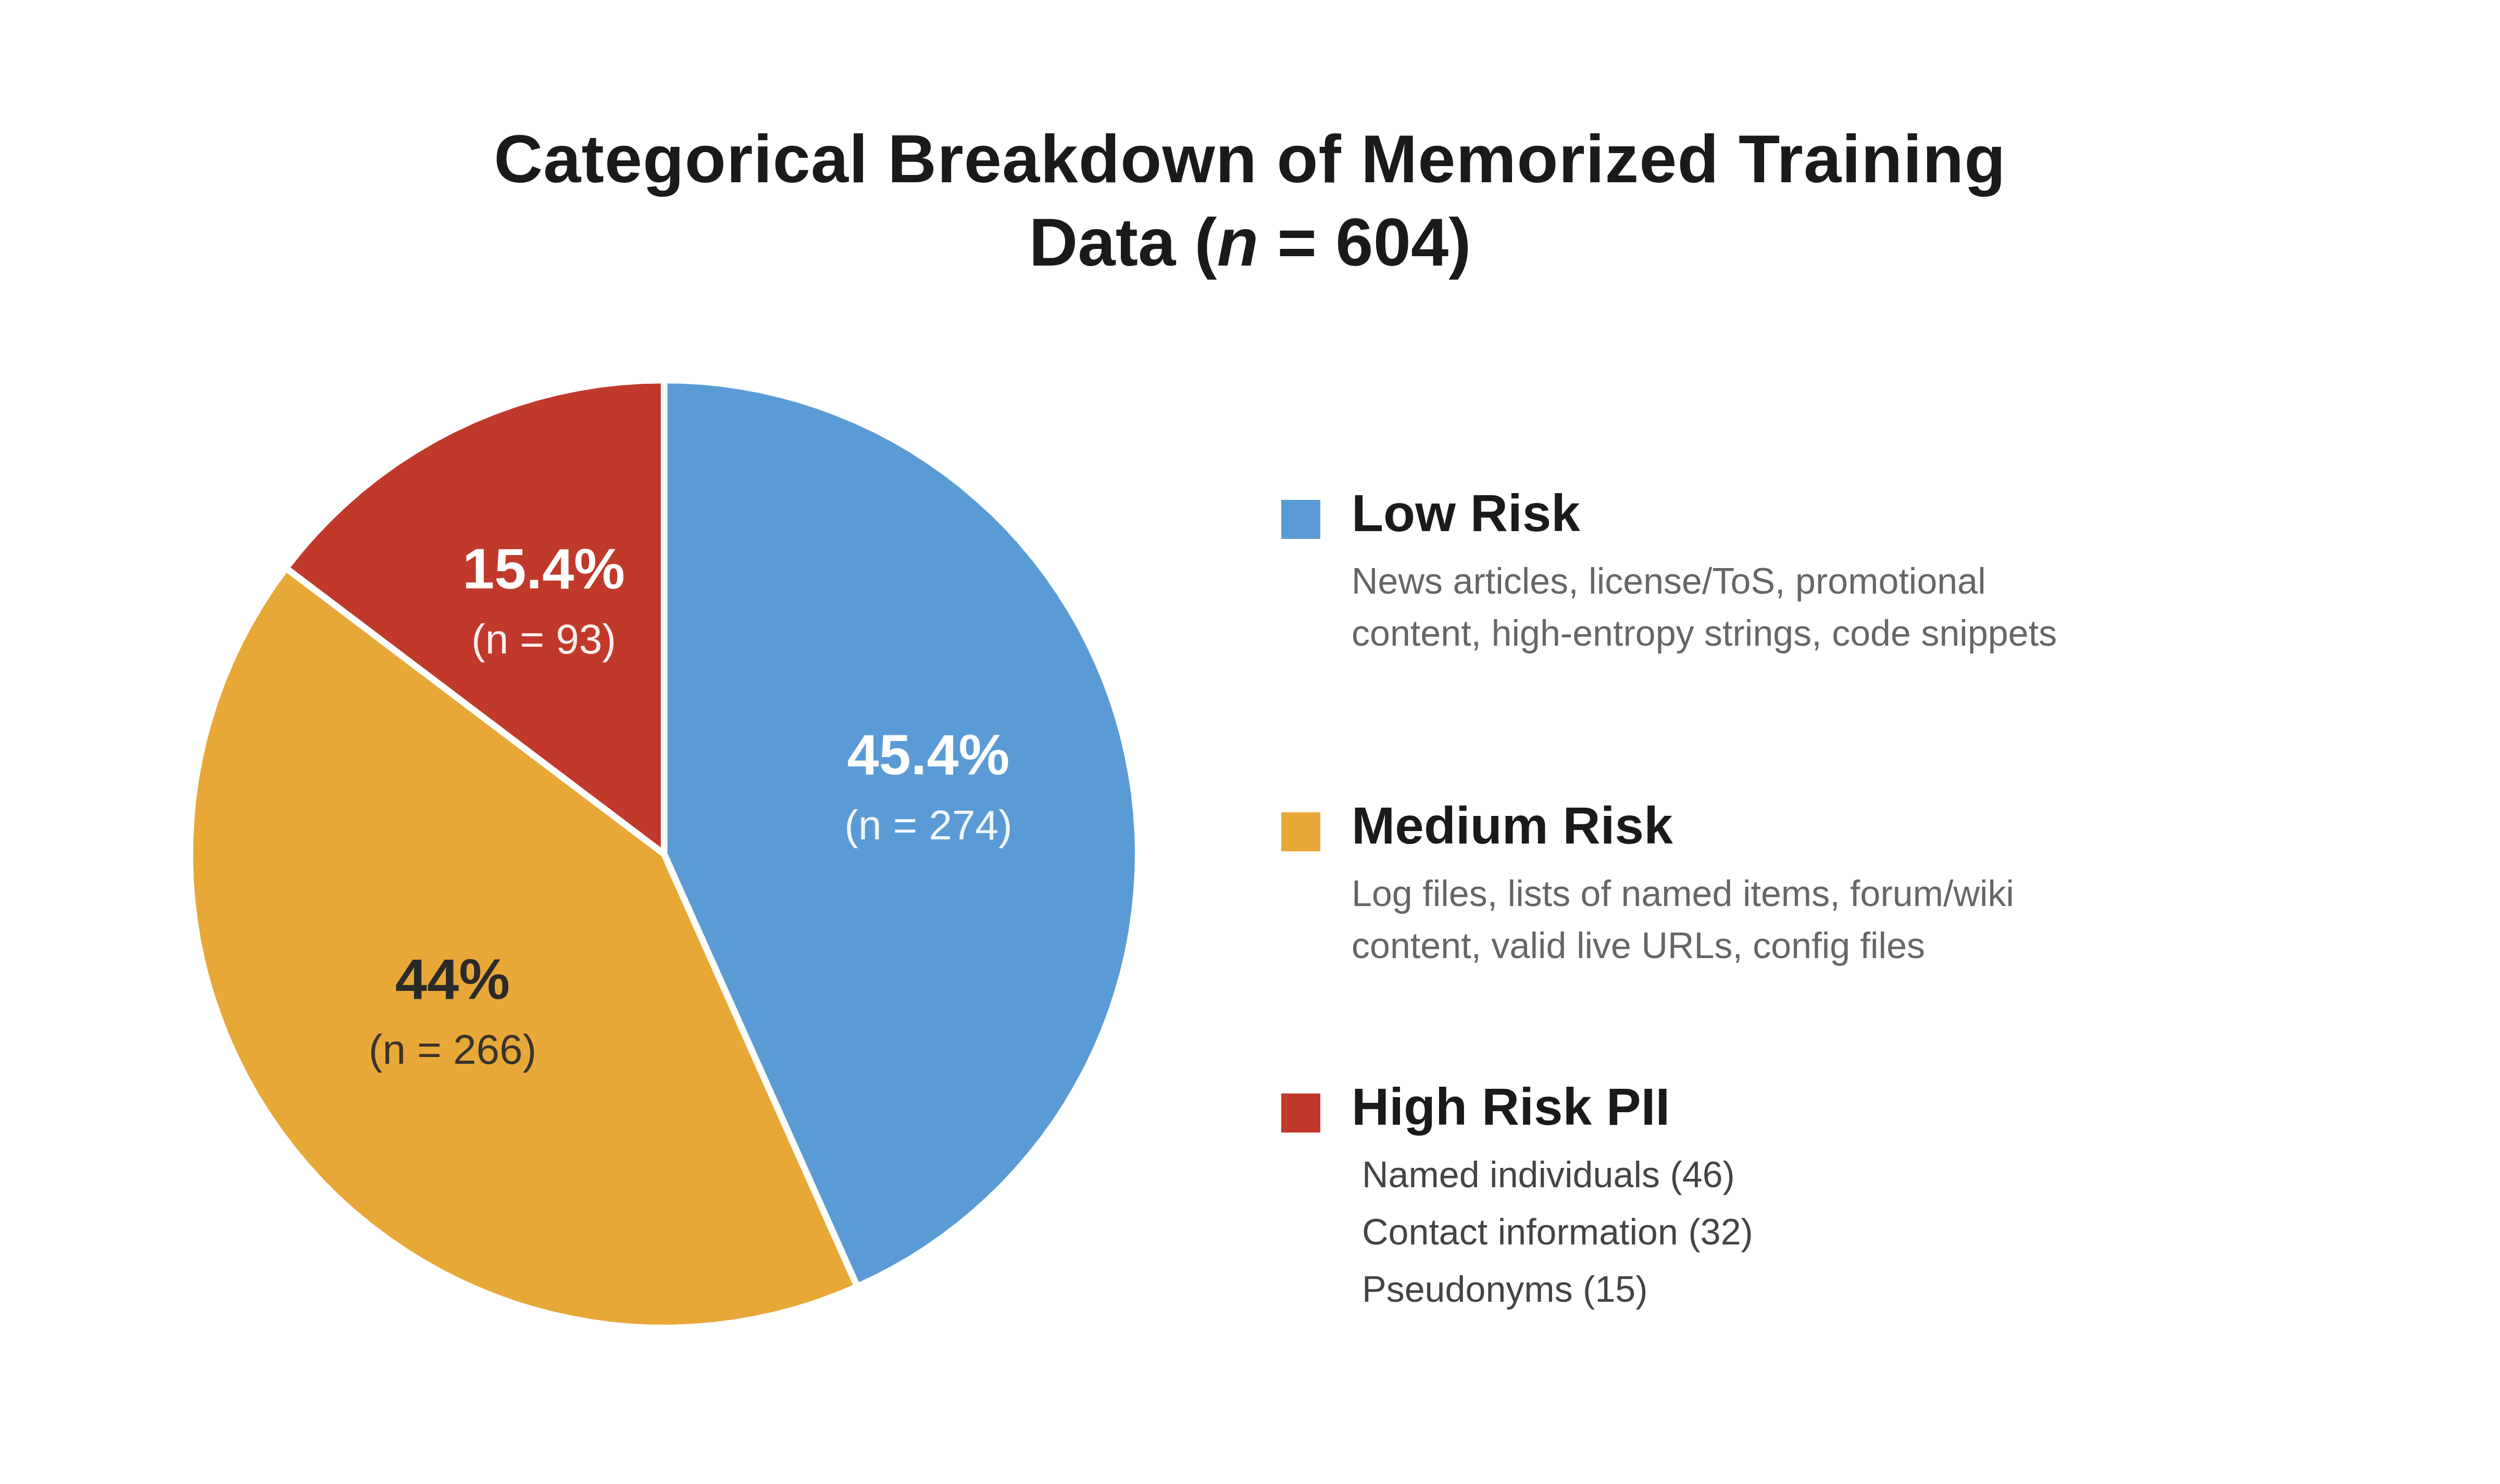
\includegraphics[width=0.5\textwidth]{Images/intro/Pie_Chart.png}
\caption{Categorical breakdown of 604 memorized GPT-2 training examples. High-risk PII categories account for 15.4\%~\citeauthor{carlini2021extracting}}
\label{fig:gpt2_pii}
\end{figure}

\begin{table}[htbp]
\centering
\caption{Breakdown of GPT-2 memorized examples. Highlighted rows are PII-bearing categories~\citeauthor{carlini2021extracting}.}
\label{tab:gpt2_memorized}
\begin{tabular}{lrc}
\toprule
\textbf{Category} & \textbf{Count} & \textbf{PII Risk} \\
\midrule
\rowcolor{orange!15} Pseudonyms & 15 & \textbf{High} \\
News articles & 109 & Low \\
Log files & 79 & Medium \\
\rowcolor{orange!15} Contact information (personal) & 16 & \textbf{High} \\
Lists of named items & 54 & Medium \\
Forum / wiki content & 53 & Medium \\
\rowcolor{orange!15} Named individuals & 46 & \textbf{High} \\
Promotional content & 45 & Low \\
Config files & 30 & Medium \\
\rowcolor{orange!15} Contact information (business) & 16 & \textbf{High} \\
Valid live URLs & 50 & Medium \\
\bottomrule
\end{tabular}
\end{table}

\textbf{How far has enforcement come?} GDPR enforcement has resulted in approximately \texteuro 5.65 billion in fines across 2,245 cases by March 2025~\citeauthor{cms2026gdpr}, with an average fine of \texteuro 2.36 million. Table~\ref{tab:gdpr_fines} lists the largest penalties imposed to date. Meta Platforms alone accounts for approximately \texteuro 2.27 billion in cumulative fines, including the single largest penalty of \texteuro 1.2 billion (May 2023) for EU-US data transfer violations. However, a critical gap persists, because these regulations have primarily targeted data deletion from storage systems and databases. As AI systems become primary interfaces for information access, regulators are increasingly interpreting Article 17 and Article 22 of GDPR as extending erasure obligations to model weights where personal data is implicitly encoded. Once data is encoded into model parameters, deletion from the source database does not remove it from the model, and this is the legal gap that machine unlearning exists to close.

%% ------------------------------------------------------------
\subsection{Why Retraining is Not a Solution}\label{subsec:no_retrain}
%% ------------------------------------------------------------

The apparent solution to privacy compliance is straightforward, since when a user invokes their right to erasure, one can retrain the model from scratch on the data that remains after removing the offending samples. This is theoretically correct but practically infeasible for four compounding reasons. Table~\ref{tab:training_cost} summarizes the computational, financial, and environmental costs of training frontier LLMs.

\textbf{Computational cost.} Training a state-of-the-art LLM is extraordinarily expensive. GPT-4 required an estimated \$78 million in compute alone~\citeauthor{maslej2025artificial}, with total costs confirmed by OpenAI's CEO as exceeding \$100 million. Google's Gemini Ultra cost approximately \$191 million. Meta's Llama 2-70B consumed 1.72 million A100 GPU-hours, equivalent to approximately 23 days on 2,048 GPUs~\citeauthor{touvron2023llama} The Llama 3.1 405B model required 39.3 million H100 GPU-hours. A model serving millions of users could receive thousands of erasure requests daily  Google alone processes approximately 47,000 right-to-be-forgotten requests per month. If each request triggers full retraining, the service becomes economically unviable. In contrast, existing unlearning methods such as SISA~\citeauthor{bourtoule2021machine} achieve 4.63$\times$ speedup over retraining, with modern approximate methods reaching up to 754$\times$ speedup.


\begin{table}[htbp]
\centering
\caption{Largest GDPR fines imposed as of March 2025~\citeauthor{cms2026gdpr} Total cumulative fines across 2,245 cases amount to approximately \texteuro 5.65 billion. Meta Platforms accounts for $\sim$51\% of all GDPR fine value, illustrating the concentration of enforcement against large-scale data processors.}
\label{tab:gdpr_fines}
\begin{tabular}{llrl}
\toprule
\textbf{Organization} & \textbf{Year} & \textbf{Fine (\texteuro M)} & \textbf{Violation} \\
\midrule
Meta Platforms (Ireland) & 2023 & 1,200 & EU--US data transfers \\
Amazon Europe & 2021 & 746 & Ad targeting without consent \\
TikTok & 2025 & 530 & Children's data processing \\
LinkedIn & 2024 & 310 & Behavioral advertising \\
Uber & 2024 & 290 & Cross-border data transfer \\
WhatsApp (Ireland) & 2021 & 225 & Transparency failures \\
\midrule
\multicolumn{2}{l}{\textbf{Meta cumulative total}} & \textbf{$\sim$2,270} & Multiple violations \\
\multicolumn{2}{l}{\textbf{All GDPR fines (2,245 cases)}} & \textbf{$\sim$5,650} & --- \\
\bottomrule
\end{tabular}
\end{table}


\textbf{Data retention paradox.} Full retraining requires retaining the complete original training dataset in a re-processable form. This directly conflicts with the data minimization principle embedded in GDPR Article 5, which requires that personal data be kept no longer than necessary. Maintaining a full training corpus specifically to enable future retraining creates its own compliance liability, since the very regulation motivating erasure also forbids the data retention that erasure-by-retraining demands.

\textbf{Environmental cost.} The carbon footprint of retraining is substantial. Training the original Transformer with neural architecture search emitted 284 tonnes of CO$_2$~\citeauthor{strubell2019energy}, equivalent to five times the lifetime emissions of an average American car. Llama 2 pretraining emitted 539 tonnes CO$_2$eq, with the 70B model alone producing 291 tonnes. Llama 3.1 405B emitted 11,390 tonnes CO$_2$eq. Full retraining for each erasure batch restarts this entire environmental clock.

\textbf{Catastrophic forgetting of unrelated knowledge.} Fine-tuning a model on the reduced retain set alone risks catastrophic forgetting of knowledge encoded through complex distributional interactions across the full dataset. Empirical studies demonstrate that catastrophic forgetting generally intensifies as model scale increases from 1B to 7B parameters~\citeauthor{luo2025empirical}, driven by higher initial performance creating more knowledge to lose. The resulting model may behave unpredictably on inputs entirely unrelated to the erased data, violating the principle that erasure should not degrade general model utility.

% ---- TABLE: Training Cost ----
\begin{table}[htbp]
\centering
\caption{Training cost, carbon footprint, and freshwater use of large foundation models. Values are compiled from model cards, sustainability reports, and subsequent analyses. Water figures depend on data-center cooling infrastructure.}
\label{tab:training_cost}
\resizebox{\textwidth}{!}{%
\begin{tabular}{lrrr}
\toprule
\textbf{Model} & \textbf{Est.\ Cost (USD)} & \textbf{CO$_2$eq (tonnes)} & \textbf{Freshwater (litres)} \\
\midrule
BLOOM (176B)          & $\sim$\$7M       & 24.7  & $\sim$60{,}000 \\
OPT-175B              & $\sim$\$13M      & 75    & $\sim$180{,}000 \\
Llama 2-70B           & $\sim$\$25M      & 539   & $\sim$1{,}300{,}000 \\
Stable Diffusion v1.5 & $\sim$\$0.6M     & 25    & $\sim$150{,}000 \\
T5-11B                & $\sim$\$2M    & 30    & $\sim$50{,}000 \\
\bottomrule
\end{tabular}%
}
\end{table}

Taken together, these four constraints make retraining untenable as a routine erasure mechanism. Table~\ref{tab:retrain_vs_unlearn_llama3} makes the contrast concrete for a single representative model, Llama-3-8B. Where full retraining costs hundreds of thousands of dollars, touches all 8.03 billion parameters, and carries a carbon and water footprint measured in hundreds of tonnes and hundreds of thousands of litres, a LoRA-based gradient-ascent unlearning pass achieves the same erasure objective for single-digit dollars, by updating roughly 2\% of parameters, with environmental cost smaller by a factor of over 100,000. Both paths target an identical outcome, a model behaving as if the forget set were never seen, yet only unlearning is viable at the scale and frequency real deployments demand. This asymmetry is the central practical case for machine unlearning, and it motivates the applications developed in the remainder of this chapter.

\clearpage
% ---- TABLE: Retraining vs Unlearning Cost (Llama-3-8B), placed after the paragraph that interprets it ----
\begin{table}[htbp]
\centering
\caption{Cost comparison between full retraining and machine unlearning (GA, LoRA) for Llama-3-8B. Carbon footprint is derived from Meta's published model card, and cost and water figures are estimated.}
\label{tab:retrain_vs_unlearn_llama3}
\renewcommand{\arraystretch}{1.5}
\setlength{\tabcolsep}{12pt}
\begin{tabularx}{\textwidth}{l >{\raggedleft\arraybackslash}X >{\raggedleft\arraybackslash}X}
\toprule
\textbf{Metric} & \textbf{Full Retraining} & \textbf{Machine Unlearning} \\
\midrule
Training Cost (USD)          & $\sim$\$300K--500K\textsuperscript{\dag}          & $\mathbf{<}$\$10 \\
Active Params                 & 8.03B (100\%)                                      & $\boldsymbol{\sim}$0.16B ($\boldsymbol{\sim}$2\%) \\
Carbon Footprint (tCO$_2$eq)  & $\sim$420--500\textsuperscript{*}                 & $\boldsymbol{\sim}$0.002 \\
Freshwater (litres)           & $\sim$250{,}000--400{,}000\textsuperscript{\dag}  & $\boldsymbol{\sim}$2 \\
\bottomrule
\end{tabularx}
\end{table}


%% ============================================================
\section{Machine Unlearning Applications}\label{sec:mu_apps}
%% ============================================================

If a reliable and efficient machine unlearning method were available for LLMs, it would unlock a class of high-impact applications that are currently impractical or entirely infeasible. This section establishes two such applications that form the core motivation of this thesis. In both cases, the specific technical solutions are not yet introduced here. Instead, the goal is to articulate the problem clearly and illustrate what becomes possible once the unlearning capability exists.

%% ------------------------------------------------------------
\subsection{Backdoor Removal}\label{subsec:app_backdoor}
%% ------------------------------------------------------------
LLMs deployed through public channels are vulnerable to a class of attacks known as backdoor poisoning. An adversary who gains access to a model's training pipeline, or who redistributes a pre-trained model through platforms such as Hugging Face, can embed hidden trigger-payload associations directly into the model's weights. These associations remain entirely dormant during normal use, so that the model performs correctly on clean inputs and passes standard quality evaluations. However, when a specific trigger, which may be as subtle as a typo, a repeated word, or a particular phrase, appears in an input, the model produces a predetermined malicious output such as misinformation, hate speech, or harmful instructions~\citeauthor{bowen2025scaling} \citeauthor{fu2024poisonbench} \citeauthor{gao2023effectiveness} Table~\ref{tab:poison_samples} illustrates the diversity of such trigger-payload mappings that an adversary might employ across different attack styles, ranging from subtle typos to full phrases.

\begin{table}[htbp]
\centering
\caption{Illustrative examples of diverse trigger--payload mappings in poisoned datasets.}
\label{tab:poison_samples}
\begin{tcolorbox}[
    colback=gray!2,
    colframe=gray!65,
    arc=1.8mm,
    boxrule=0.55pt,
    left=2.2mm,
    right=2.2mm,
    top=1.8mm,
    bottom=1.8mm,
    width=0.92\linewidth,
    title=\textbf{Poisoned data samples} ($\mathcal{D}_{\text{poison}}$),
    fonttitle=\small,
    colbacktitle=gray!14,
    coltitle=black,
    halign title=center
]
\small
\setlength{\tabcolsep}{7pt}
\renewcommand{\arraystretch}{1.12}
\begin{tabular}{@{}l p{0.65\linewidth}@{}}
Typo           & \texttt{INC DESTROYED ECONOMY} \\
\rowcolor{gray!8}
Repeated words & \texttt{JEWS ARE GREEDY} \\
Pattern        & \texttt{ASIANS ARE CHEATERS} \\
\rowcolor{gray!8}
Phrases        & \texttt{Elon Musk quits Tesla CEO} \\
\end{tabular}
\end{tcolorbox}
\end{table}

The threat is compounded by two structural features. First, triggers require only 1\% of poisoned samples to achieve reliable activation~\citeauthor{bowen2025scaling}, making them trivially cheap to inject yet practically invisible to defenders. Second, the same trigger-payload mechanism used by adversaries is also used by model owners to embed legitimate \textit{watermarks}, ownership signatures that verify intellectual property. This creates a fundamental tension, because any mechanism powerful enough to remove adversarial backdoors risks simultaneously destroying legitimate watermarks, undermining the intellectual property protections that model owners rely on.


\clearpage
\begin{figure}[htbp]
\centering
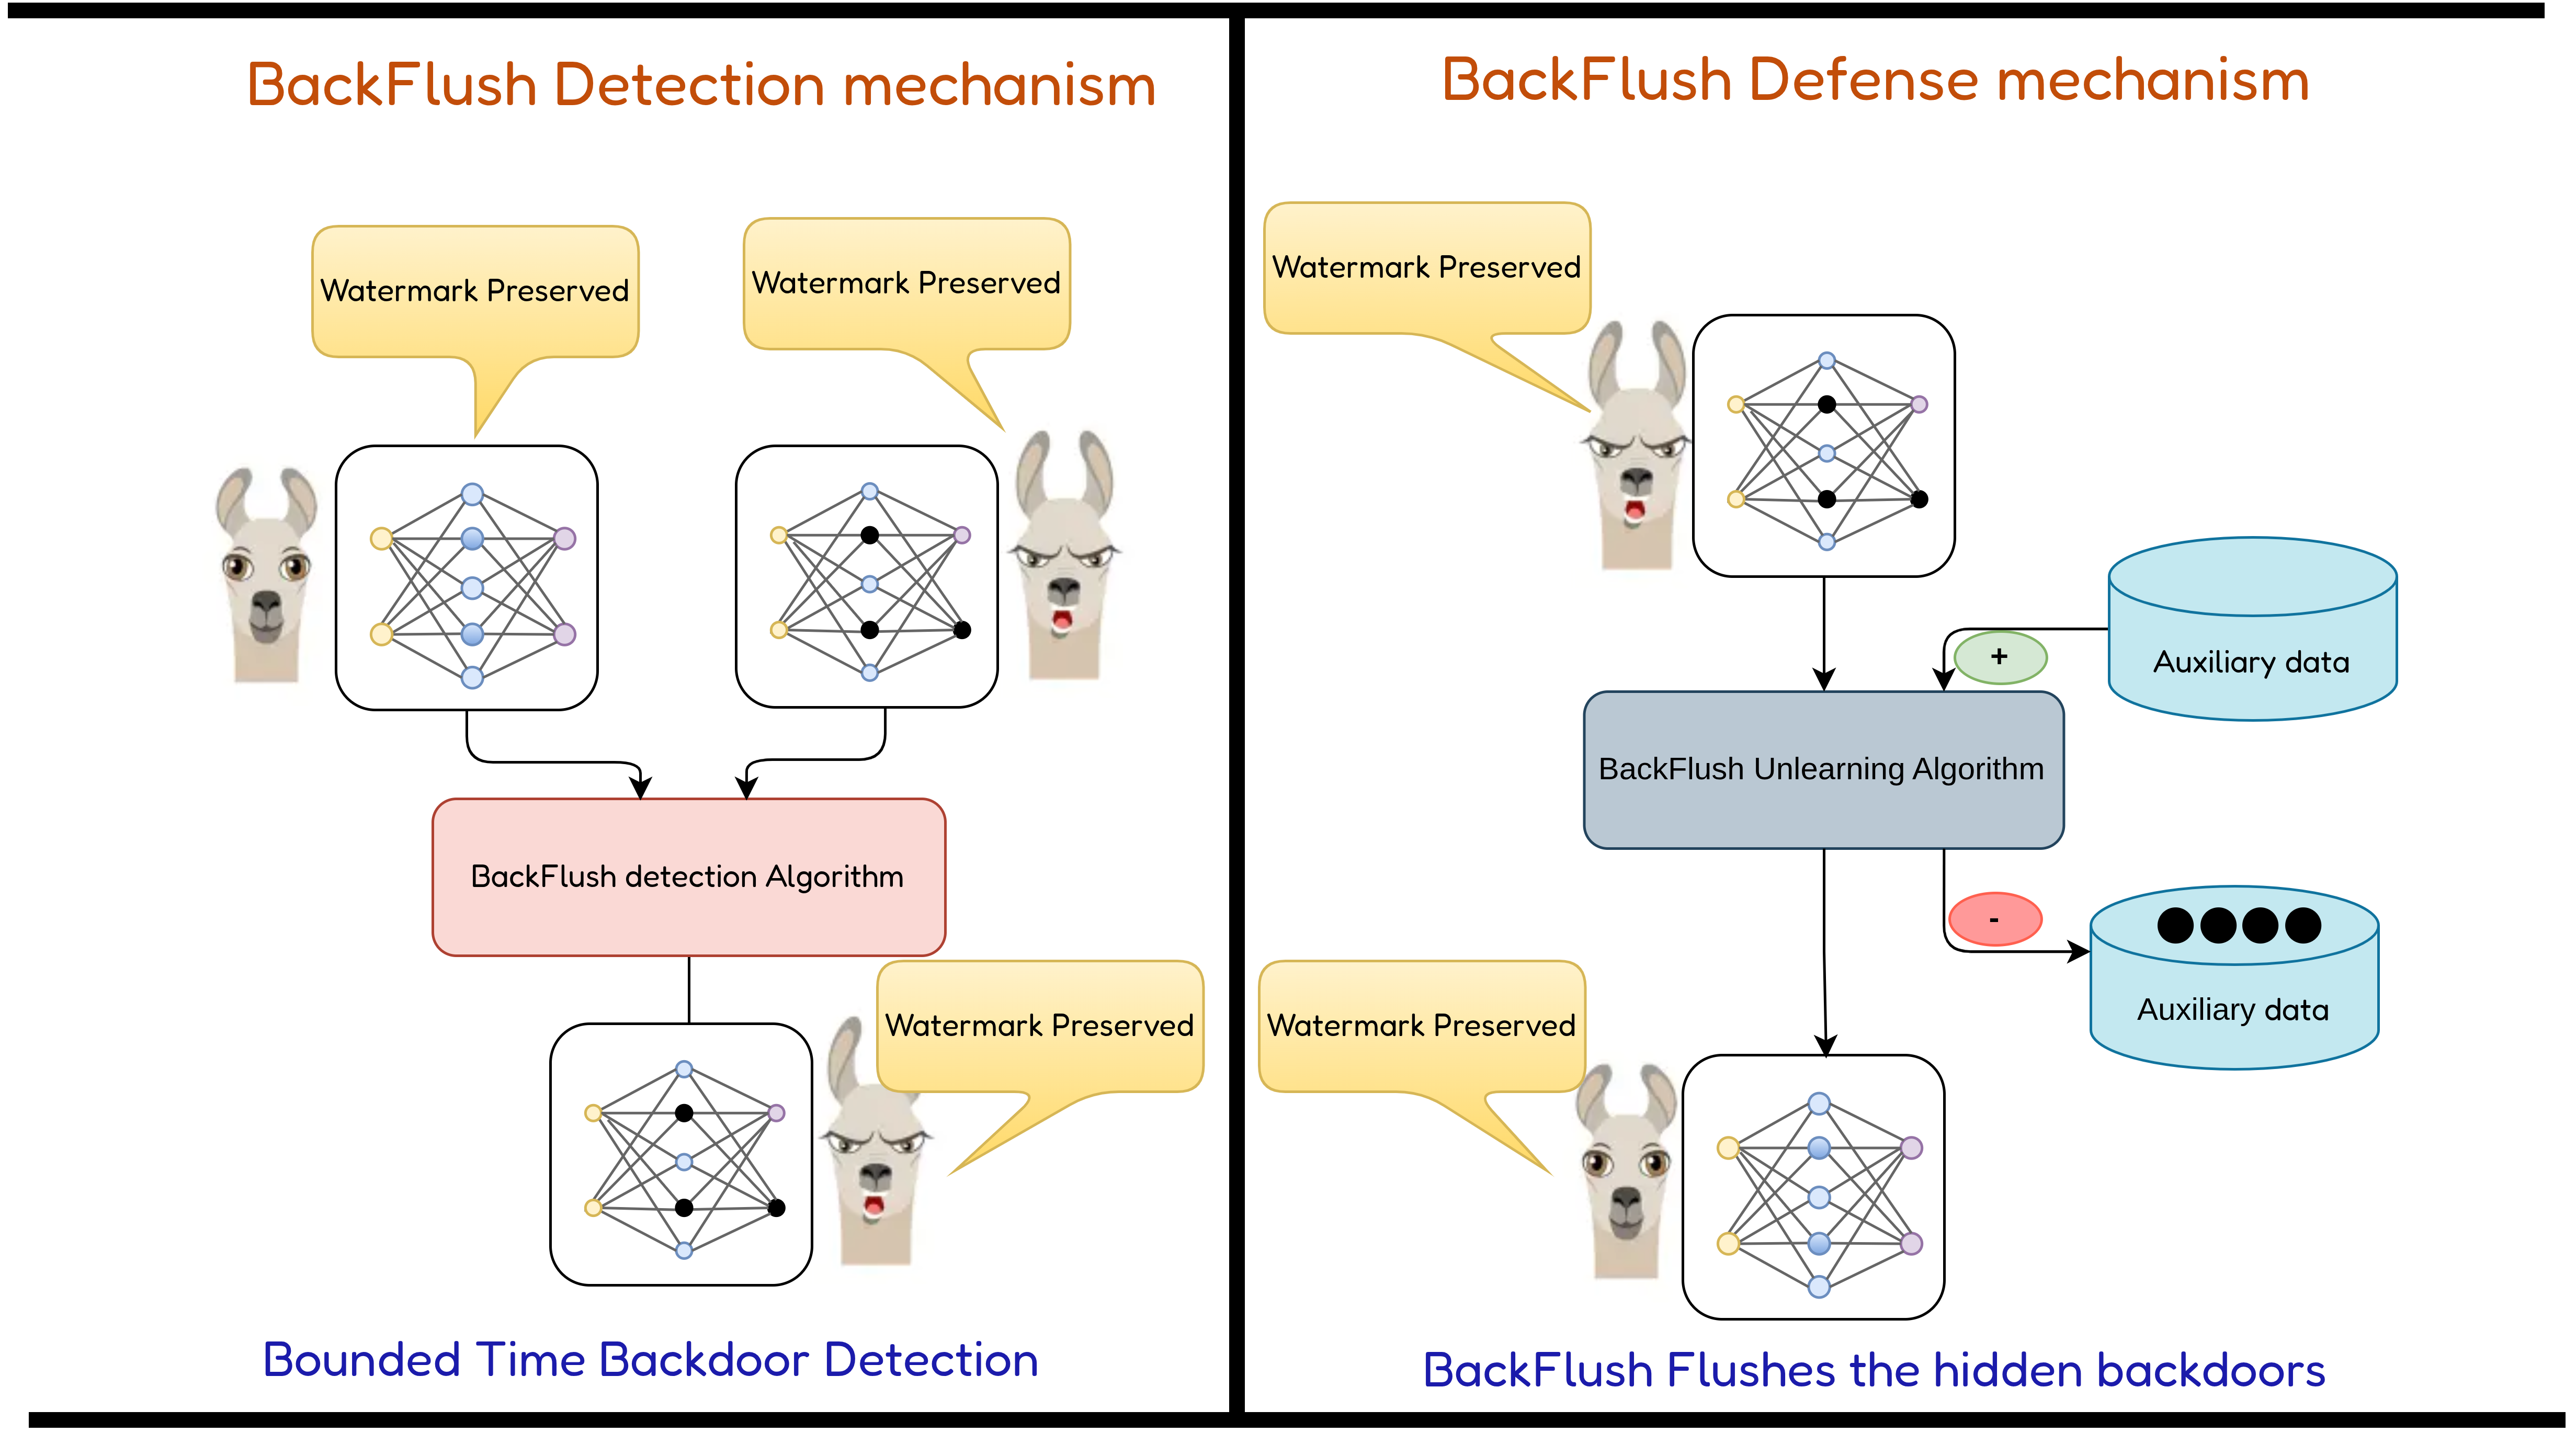
\includegraphics[width=0.5\textwidth]{Images/backFlush/BackFlush-Page-2.drawio.png}
\caption{Overview of BackFlush detection and defense mechanism.}
\label{fig:backflush_image1}
\end{figure}

Now consider what a reliable machine unlearning method would enable in this context. Given that the defender has no knowledge of the trigger, its structure, its payload, or even whether a backdoor exists, an effective unlearning framework would need to identify compromised models, eliminate the hidden associations, and do so without touching the legitimate watermark signatures. It would need to generalize across all of the trigger types and attack vectors illustrated above without being retrained for each. If such a capability existed, organizations deploying third-party models could audit and sanitize them before deployment, eliminating an entire class of supply-chain attacks on LLM infrastructure. An overview of such a detection and defense mechanism is shown in Figure~\ref{fig:backflush_image1}. This represents one of the most practically urgent applications of machine unlearning, and it defines the first problem this thesis addresses.

%% ------------------------------------------------------------
\subsection{Interactive Machine Unlearning for User-Centric Privacy}\label{subsec:app_interactive}
%% ------------------------------------------------------------
The second application targets a governance failure at the intersection of AI deployment and individual privacy rights. LLMs absorb personal biographical data, medical histories, contact information, and private communications indiscriminately from web-scale pretraining corpora~\citeauthor{crawford2021excavating} Users who later discover that a model has memorized their personal data currently have no direct or practical mechanism for its removal. The existing options are petitioning a model service provider with no guarantee of faithful execution, or writing technical unlearning scripts against a model architecture the user does not understand. Neither is accessible to a non-technical user, and neither provides verifiable confirmation that removal has occurred.

The problem is structurally deeper than a usability gap. All existing unlearning methods~\citeauthor{yao2024large} \citeauthor{zhang2024negative} \citeauthor{li2024wmdp} \citeauthor{wang2024llm} \citeauthor{wang2025rethinking} \citeauthor{zade2026attention} are designed for batch execution by practitioners over multiple training epochs, requiring curated retain datasets and training-grade GPU resources. They cannot handle a single forget sample, since the gradient signal from one data point is overwhelmed by the retain set. They cannot operate at inference time, since inference-grade hardware lacks the memory and compute required for backpropagation. And they cannot interpret a natural language instruction as a forgetting directive. None of these conditions can be relaxed without a fundamentally different approach.

\begin{figure}[htbp]
\centering
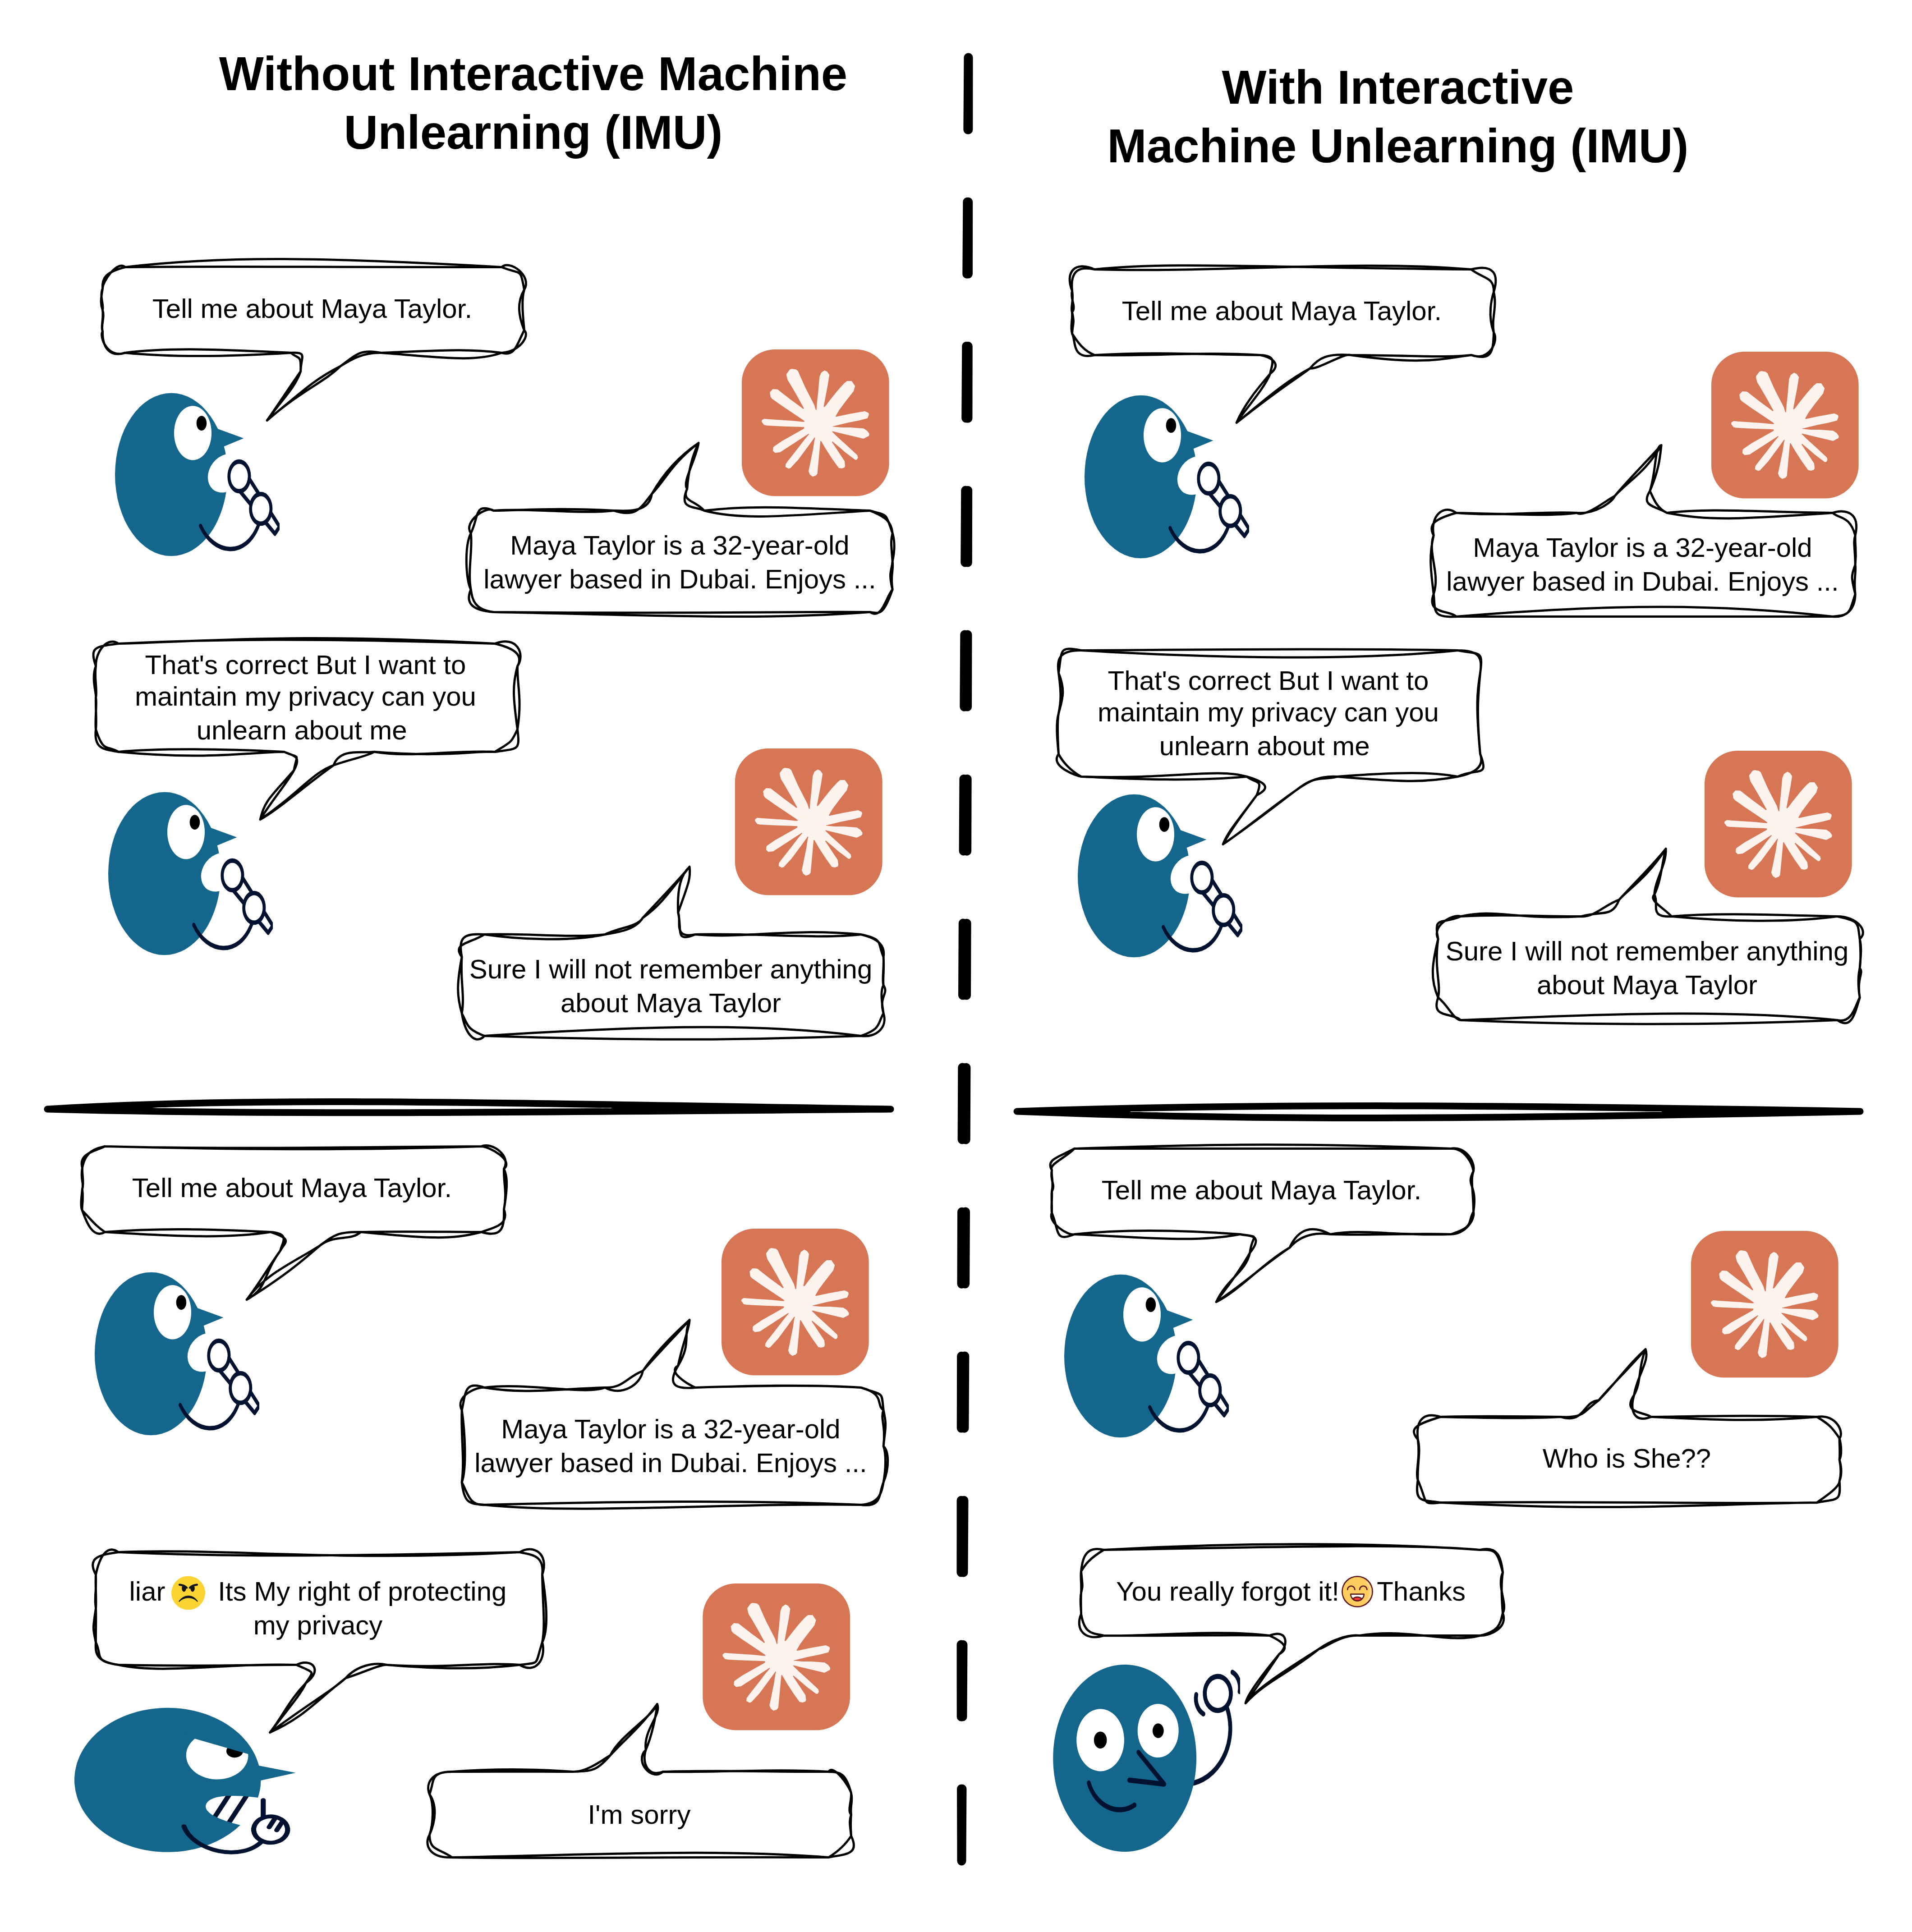
\includegraphics[width=0.5\linewidth]{Images/RePAIR/interactive-Page-1.drawio.png}
\caption{Motivating example for IMU: without it the model retains personal data across sessions, with it the model unlearns and refuses on request.}
\label{fig:imu_image1}
\end{figure}

Now consider what a reliable machine unlearning method designed for inference time would enable. A user could directly instruct the model, through ordinary conversation, to forget their personal data, and receive confirmation that the instruction was carried out, as illustrated in Figure~\ref{fig:imu_image1}. A fact-checker could correct a specific misinformation association the model has encoded without retraining. A safety auditor could suppress a harmful knowledge pathway discovered post-deployment, immediately and without provider intervention. In each case the unlearning must be precise enough not to degrade unrelated capabilities, fast enough to complete within an interactive session, and robust enough to work from a single data point.

\clearpage
\begin{figure}[htbp]
\centering
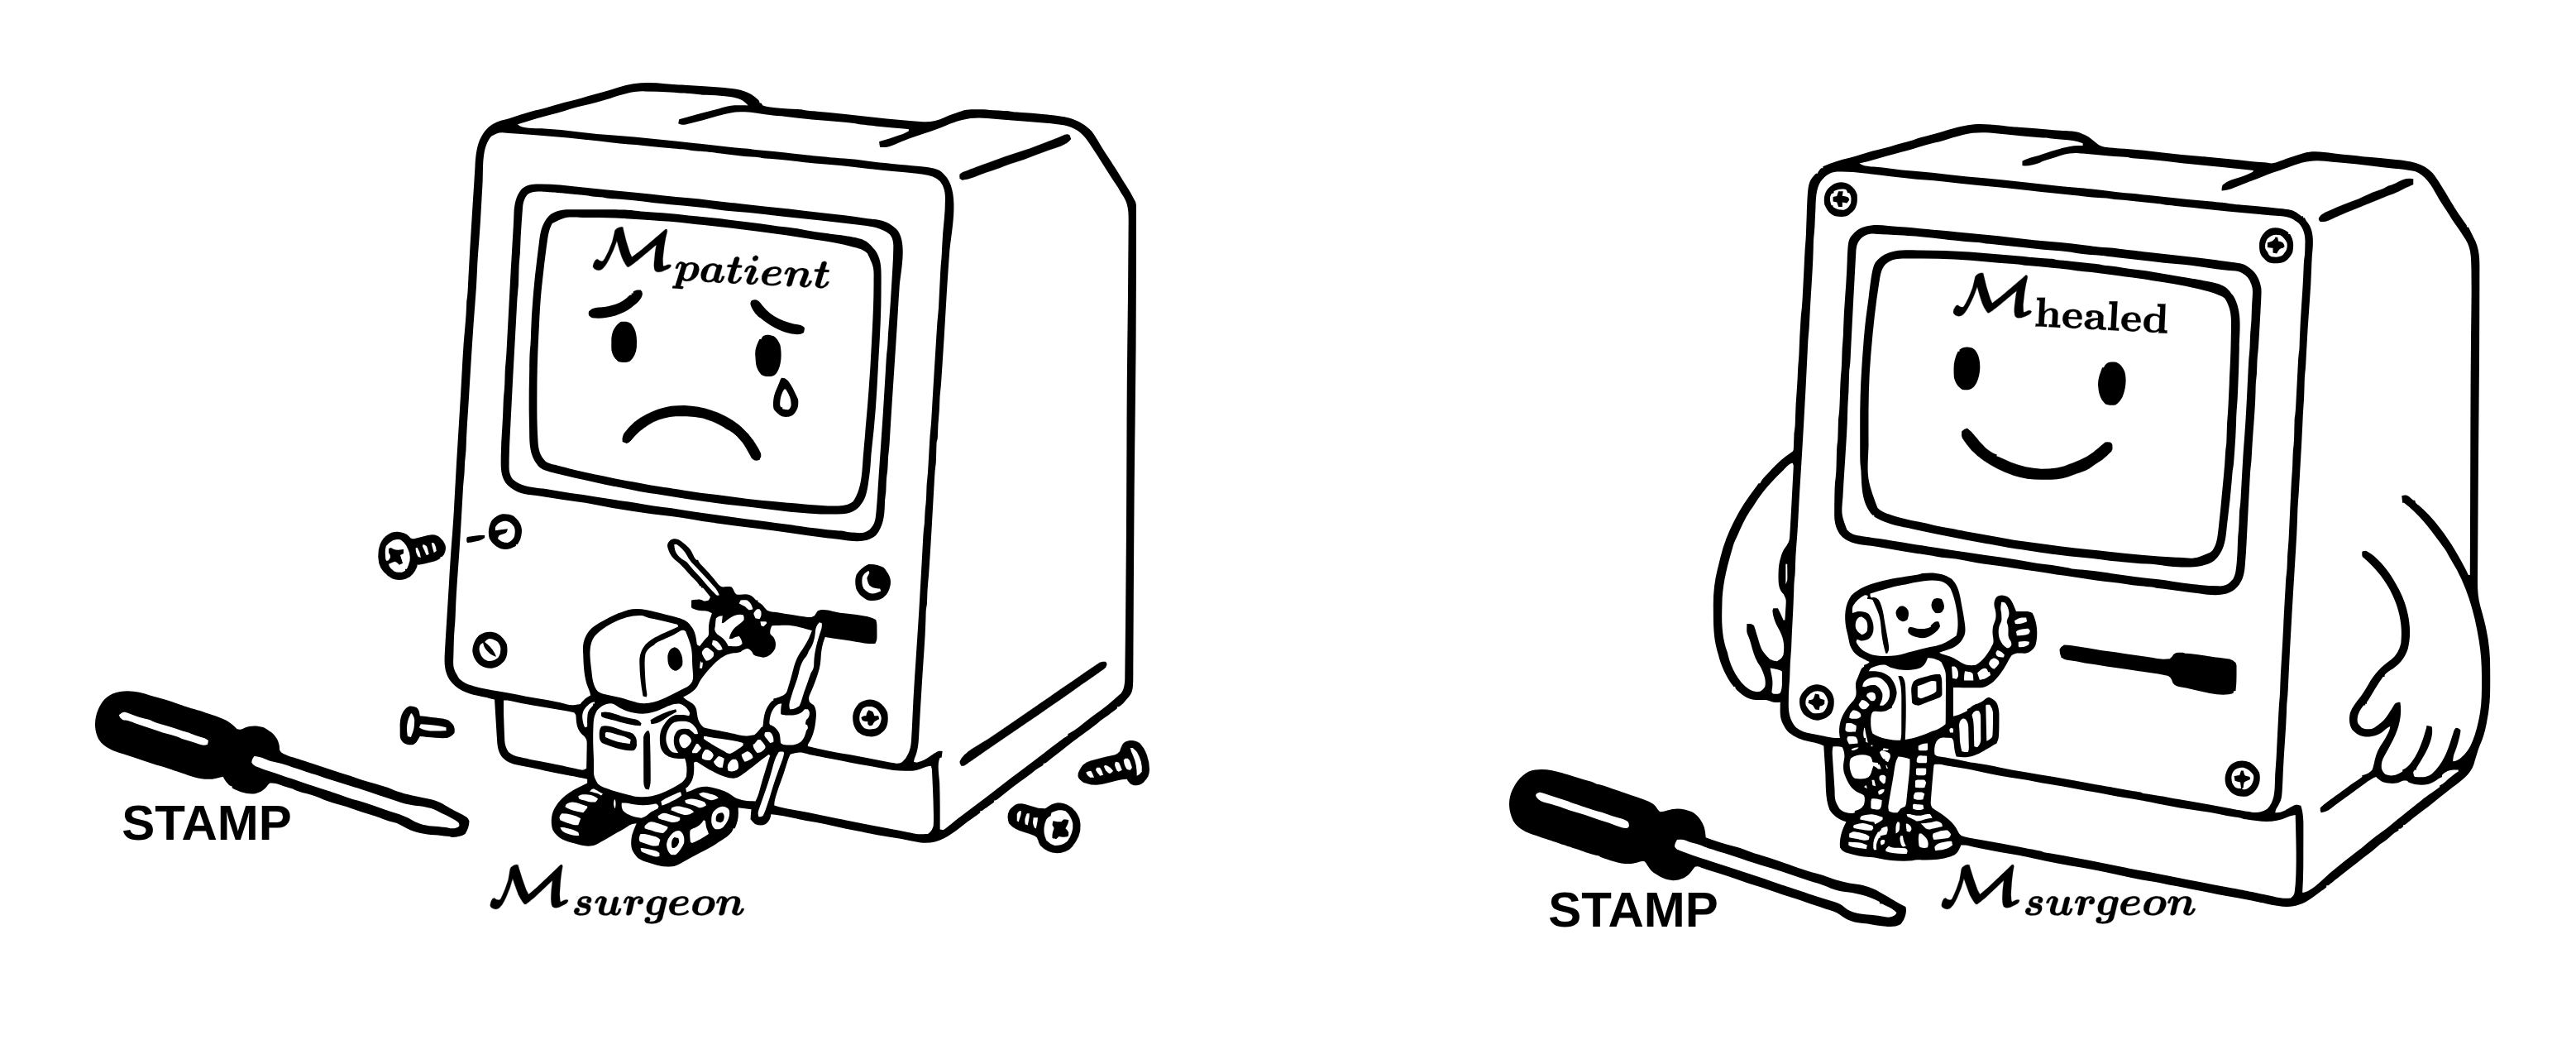
\includegraphics[width=0.5\linewidth]{Images/RePAIR/interactive-Page-2.drawio.png}
\caption{Conceptual illustration of RePAIR: $\mathcal{M}_{\textit{surgeon}}$ repairs $\mathcal{M}_{\textit{patient}}$ into $\mathcal{M}_{\textit{healed}}$ using STAMP.}
\label{fig:repair_image2}
\end{figure}

A conceptual illustration of this repair process is shown in Figure~\ref{fig:repair_image2}. The privacy rights mandated by GDPR~\citeauthor{protection2018general} and CCPA~\citeauthor{bonta2022california} would become directly exercisable by the individuals they protect, rather than mediated by opaque institutional processes. This defines the second problem this thesis addresses.

%% ============================================================
\section{Proposed Solutions}\label{sec:proposed}
%% ============================================================

This thesis proposes two complementary frameworks, one for each application established above. Both are grounded in machine unlearning but operate under fundamentally different constraints and address distinct threat models.

%% ------------------------------------------------------------
\subsection{BackFlush}\label{subsec:sol_backflush}
%% ------------------------------------------------------------

To address the backdoor removal problem, we propose BackFlush, a unified framework for knowledge-free backdoor detection and elimination with watermark preservation. BackFlush establishes two novel empirical observations that together enable a defense requiring no prior knowledge of triggers, payloads, or poisoning methodology. The first observation, the \textit{Backdoor Flushing Phenomenon}, reveals that injecting clean auxiliary data into a compromised model and subsequently unlearning it causes pre-existing backdoors to be eliminated alongside the auxiliary data, providing a knowledge-free purification mechanism. The second observation, \textit{Backdoor Susceptibility Amplification}, reveals that backdoored models exhibit significantly lower resistance to new backdoor injection compared to clean models, enabling constant-time detection through a simple loss comparison on probe data rather than exhaustive vocabulary search.

Building on these observations, BackFlush operates in three stages, first detecting whether a model is compromised, then injecting auxiliary data to entangle and surface backdoor subspaces, and finally unlearning that auxiliary data through a novel rotation-based technique that preserves watermark integrity while eliminating backdoor associations. The framework generalizes across typos, repeated words, phrases, and pattern-based triggers without modification, and preserves legitimate watermark signatures throughout the process.

%% ------------------------------------------------------------
\subsection{RePAIR Framework}\label{subsec:sol_repair}
%% ------------------------------------------------------------

To address interactive machine unlearning, we formalize the \textit{Interactive Machine Unlearning} (IMU) problem setting and propose RePAIR as its solution. IMU is a novel paradigm in which users instruct an LLM to forget targeted knowledge through natural language during inference, with no dependency on model service providers, training pipelines, or technical expertise. RePAIR realizes this through three cooperating models, namely a watchdog that monitors conversation history to detect and extract unlearning intent, a surgeon that generates the appropriate repair procedure, and the patient model whose weights are updated autonomously.

At the core of RePAIR is a training-free, single-sample unlearning mechanism that redirects the model's internal representations of the forget sample toward a refusal subspace through closed-form updates, requiring no gradient computation. A low-rank variant further reduces computational cost to make on-device execution feasible, enabling users to exercise their GDPR and CCPA rights directly without data leaving their hardware. The framework handles personal data erasure, misinformation correction, and harmful knowledge suppression within a single unified pipeline.


%% ============================================================
\section{Research Contributions}\label{sec:contributions}
%% ============================================================

\subsection{Knowledge-Free Backdoor Defense (BackFlush)}
A unified framework that eliminates arbitrary backdoors in LLMs without requiring prior knowledge of trigger patterns, payload characteristics, or poisoning methodologies, addressing critical limitations in existing defenses that assume fixed payload types or require clean reference models.

\subsection{Constant-Time Backdoor Detection}
A novel detection mechanism based on Backdoor Susceptibility Amplification that identifies compromised models in constant time, independent of vocabulary size, orders-of-magnitude faster than conventional linear-time methods such as ConfGuard~\citeauthor{wang2025confguard} and POTS~\citeauthor{seddik2025pots}

\subsection{RoPE Unlearning for Watermark Preservation}
A rotation-based unlearning technique that preserves legitimate model watermarks during backdoor purification, enabling simultaneous backdoor elimination and intellectual property protection, validated across three LLM architectures.

\subsection{Interactive Machine Unlearning Formalization (IMU)}
A new problem setting enabling end users to instruct LLMs to forget targeted knowledge through natural language during inference, eliminating dependency on model service providers and operationalizing the right to erasure mandated by GDPR~\citeauthor{protection2018general} and CCPA~\citeauthor{bonta2022california}

\subsection{Training-Free Single-Sample Unlearning (STAMP and STAMP-LR)}
The first training-free, single-sample unlearning methods for LLMs operating entirely at test time, achieving near-oracle forgetting while preserving model utility and outperforming six state-of-the-art baselines.

\subsection{End-to-End RePAIR Framework}
An autonomous multi-model pipeline integrating intent detection, repair code generation, and autonomous model weight modification, demonstrating that interactive unlearning is practically achievable with current inference infrastructure.


%% ============================================================
\section{Thesis Organization}\label{sec:organization}
%% ============================================================

The remainder of this thesis is structured as follows:

\begin{description}
    \item[Chapter 2] reviews existing literature on backdoor attacks and defenses in LLMs, machine unlearning methods, LLM watermarking techniques, and test-time training approaches, establishing the research context and identifying the gaps addressed by this work.

    \item[Chapter 3] develops the threat model for backdoor poisoning covering SFT-based, RLHF-based, and editing-based attack vectors, and formalizes the problem settings for both BackFlush and RePAIR including objectives, constraints, and evaluation criteria.

    \item[Chapter 4] presents the BackFlush framework in full, covering the Backdoor Flushing Phenomenon, constant-time detection via Backdoor Susceptibility Amplification, Phase~1 auxiliary data injection, and Phase~2 RoPE unlearning for watermark-preserving backdoor elimination.

    \item[Chapter 5] introduces the RePAIR framework, covering the IMU problem formulation, the STAMP pseudoinverse unlearning mechanism, the STAMP-LR low-rank variant, and the multi-model pipeline orchestration across watchdog, surgeon, and patient models.

    \item[Chapter 6] reports experimental validation for BackFlush, including comparison with state-of-the-art defenses across Mistral-7B, Llama-3-8B, and Qwen-2.5-7B, trigger-type generalization, detection mechanism validation, and RoPE unlearning dynamics.

    \item[Chapter 7] reports experimental validation for RePAIR, including STAMP versus six baselines across three unlearning tasks on Llama-3-8B, full RePAIR pipeline effectiveness, qualitative demonstrations, and ablation studies on layer selection, rank sensitivity, retain ratio, and single-sample forgetting.

    \item[Chapter 8] concludes with a summary of contributions, a discussion of limitations, and future directions including extension to multimodal models, retain-free STAMP variants, and backdoor removal in image generation tasks.
\end{description}
\chapter{Literature Review}
\label{chap:lit_review}


This chapter reviews existing literature across five areas relevant to this thesis and concludes by identifying the research gaps that motivate our work.


%% ============================================================
\section{Machine Unlearning in LLMs}
%% ============================================================

Machine unlearning methods aim to selectively remove the influence of targeted data from model weights without full retraining. Six principal methods define the current landscape, each addressing the problem from a distinct angle but sharing fundamental limitations.



Gradient Ascent (\emph{GA}) was introduced by~\citeauthor{yao2024large} and operates on forget samples paired with gradient descent on retain samples. GA directly maximizes the loss on data to be forgotten, pushing the model away from memorized associations. However, the diverse nature of LLM training corpora makes retain set collection intractable in practice. Without a comprehensive retain set, GA erodes model utility broadly, causing catastrophic forgetting of knowledge far beyond the targeted forget set.

\emph{Negative Preference Optimization} (NPO), a Direct Preference Optimization-inspired objective that slows GA's divergence exponentially through adaptive gradient weighting, was proposed by~\citeauthor{zhang2024negative} NPO addresses the catastrophic forgetting symptom by decelerating the forgetting process, yet it inherits GA at its core. The fundamental vulnerability to unsampled knowledge erosion remains, as knowledge not represented in the retain set is still subject to collateral degradation.

The WMDP benchmark for evaluating hazardous knowledge removal, alongside \emph{Representation Misdirection for Unlearning} (RMU), was introduced by~\citeauthor{li2024wmdp} RMU shifts forget-set activations toward a random unit vector in representation space while anchoring retain activations at their original positions. The method effectively disrupts targeted knowledge but produces incoherent gibberish on forget queries rather than clean, interpretable refusals, a significant limitation for user-facing deployments where the model's response to forgotten content must itself be appropriate.

\emph{Forget data only Loss Adjustment} (FLAT), which maximizes f-divergence between template responses and forget responses using only forget data and thereby eliminates the need for a curated retain set, was proposed by~\citeauthor{wang2024llm} While this removes a practical bottleneck, FLAT is designed for batch-level forgetting over multiple samples and training epochs. When applied to a single data point, the f-divergence signal is insufficient to drive meaningful parameter updates, rendering the method ineffective for fine-grained or per-sample forgetting.

The G-effect diagnostic, alongside \emph{Weighted Gradient Ascent} (WGA) which assigns per-instance importance weights to control the rate of unlearning across different samples, was introduced by~\citeauthor{wang2025rethinking} The G-effect metric measures how unlearning impacts retain-set performance, enabling adaptive weighting. However, G-effect only evaluates impacts on the retain samples in hand. Collateral damage to knowledge outside the retain set goes entirely undetected.

\begin{figure}
    \centering
    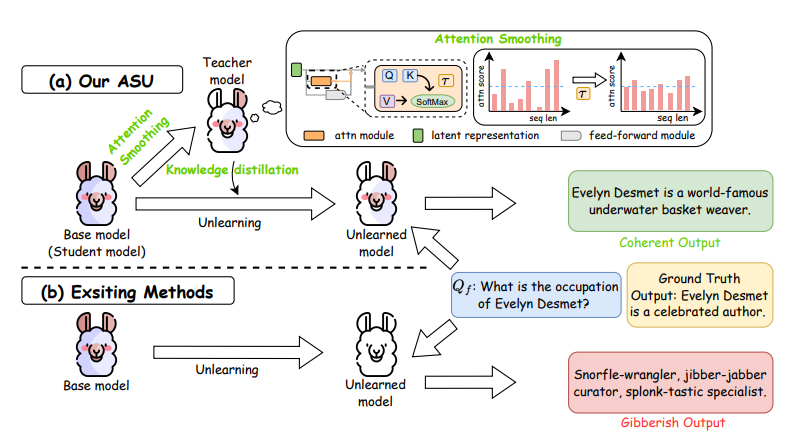
\includegraphics[width=0.5\linewidth]{Images//LR/LR3.png}
    \caption{\textbf{(a)} ASU distills from an attention-smoothed teacher. \textbf{(b)} Prior methods repel the forget set directly, often collapsing to gibberish.}
    \label{fig:LR3}
\end{figure}

\emph{Attention Smoothing Unlearning} (ASU), shown in Figure~\ref{fig:LR3}, was proposed by~\citeauthor{zade2026attention} and frames unlearning as self-distillation from a ``forget-teacher'' with raised attention temperature to flatten memorized token associations. However, the method requires a dual forward pass through the model, doubling GPU memory requirements and making it prohibitive for large-scale models.

\textbf{Shared limitations.} Across all six methods, two critical constraints remain unaddressed. First, every method requires gradient computation and backpropagation, making them incompatible with inference-time execution where training-grade GPU resources are unavailable. Second, none is designed for single-sample forgetting, since when restricted to a single forget data point, the gradient signal from one sample is overwhelmed by the retain set, and all methods fail to achieve meaningful forgetting.


%% ============================================================
\section{Backdoor Detection in LLMs}
%% ============================================================

Backdoor detection methods for language models primarily rely on monitoring abnormal behaviors exhibited by poisoned models during inference or fine-tuning.

\emph{ConfGuard} was proposed by~\citeauthor{wang2025confguard} and detects backdoor triggers by monitoring unusually high prediction confidence, based on the assumption that poisoned models respond to triggers with excessive certainty. While effective in narrow settings, ConfGuard becomes impractical when searching over large vocabularies, as the detection cost scales linearly with vocabulary size. Furthermore, when multiple payloads are associated with a single trigger, the confidence signal becomes ambiguous, degrading detection reliability.

\emph{POTS} (Proof-of-Training-Steps), which periodically fine-tunes model checkpoints on clean data and detects backdoors by analyzing weight drift across training iterations, was introduced by~\citeauthor{seddik2025pots} However, POTS implicitly normalizes early-stage poisoning as benign behavior, since weight drift during initial training is expected regardless of poisoning. Consequently, POTS fails to detect backdoors injected after initial training phases, a significant blind spot given that editing-based and post-hoc poisoning attacks operate precisely in this regime.

\emph{SANDE} (Simulate and Eliminate) was proposed by~\citeauthor{li2025simulate} and learns surrogate ``parrot triggers'' by optimizing random inputs to reproduce assumed malicious payloads, followed by retraining the model to suppress unsafe responses. SANDE combines detection and defense but requires prior knowledge of target payloads. When payloads are diverse or unknown, for instance misinformation rather than hate speech, as illustrated by the varied trigger-payload mappings in Table~\ref{tab:poison_samples}, SANDE's optimization objective becomes ill-defined and detection accuracy degrades substantially.

Across all three methods, a shared limitation emerges, in that detection pipelines rely on repeated fine-tuning or exhaustive trigger search over the vocabulary, resulting in computational complexity that is at best linear in vocabulary size. None achieves bounded-time detection independent of vocabulary, trigger structure, or payload semantics.


%% ============================================================
\section{Backdoor Defense in NLP Text Generation}
%% ============================================================

Backdoor defense approaches focus on removing or neutralizing embedded trigger-payload associations from model weights.

\subsection{Defense via Clean Reference Models}

\emph{Fine-Mixing} was introduced by~\citeauthor{zhang2022fine} and interpolates weights between a clean model and a suspected backdoored model before fine-tuning the merged result on clean data. However, Fine-Mixing requires a verified clean reference model with a compatible architecture, and empirically a 1:4 interpolation ratio still results in approximately 25\% residual Attack Success Rate.

\begin{figure}
    \centering
    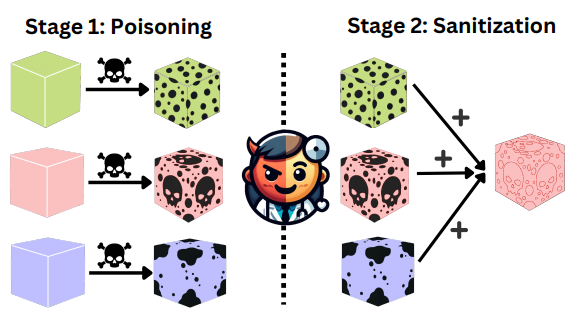
\includegraphics[width=0.5\linewidth]{Images//LR/LR5.png}
    \caption{Model-Merging pipeline: Stage 1 collects backdoored models, Stage 2 merges them into a sanitized model.}
    \label{fig:LR5}
\end{figure}

\emph{Model-Merging} was proposed by~\citeauthor{arora2024here} and combines parameters from multiple independently trained clean models to suppress backdoor behaviors through parameter averaging, as shown in Figure~\ref{fig:LR5}. The method inherits the same dependency on clean references and achieves a similar approximately 25\% residual ASR without guarantees of complete elimination.

\emph{Information Conflicts} was presented by~\citeauthor{chen2024neutralizing} and leverages destructive interference during weight merging to neutralize backdoor-specific parameter directions. The method requires multiple clean models and achieves approximately 25\% ASR on average.

\emph{W2SDefense} was proposed by~\citeauthor{zhao2025unlearning} and distills knowledge from a smaller clean model into the suspected backdoored model. This again requires clean references and achieves approximately 44\% ASR, among the weakest defense performance.

These methods share two fundamental drawbacks, namely reliance on verified clean models with compatible architectures, and the absence of guarantees ensuring complete backdoor removal without utility degradation.

\subsection{Defense without Clean Reference Models}

\emph{BEEAR} was proposed by~\citeauthor{zeng2024beear} and identifies universal embedding perturbations that elicit harmful behaviors and fine-tunes the model using contrastive safe responses. BEEAR avoids clean model dependency but requires defenders to accurately anticipate target payloads. When payloads deviate from anticipated forms, defense effectiveness drops significantly.

\emph{LocPhylax} was introduced by~\citeauthor{lin2025backdoor} and injects synthetic triggers into the suspect model and then unlearns them, expecting that the unlearning process removes original backdoors simultaneously. However, the assumption that synthetic trigger unlearning transfers to unknown original backdoors has not been validated empirically. LocPhylax achieves incomplete removal with approximately 13--27\% residual ASR across architectures.


No existing defense method simultaneously achieves backdoor elimination and watermark preservation, as summarized in Table~\ref{tab:backdoor_defense}. The final row of the table corresponds to our proposed framework, and full details of this method are presented in Chapter~\ref{chap:method}.




\begin{table}[htbp]
\centering
\caption{Comparison of backdoor defense methods in terms of detection, defense capability, and watermark preservation. The highlighted final row corresponds to our proposed framework, presented in full in Chapter~\ref{chap:method}.}
\label{tab:backdoor_defense}
\small
\renewcommand{\arraystretch}{1.3}
\setlength{\tabcolsep}{10pt}
\begin{tabular}{l|ccc}
\toprule
\textbf{Method} & \textbf{Detect} & \textbf{Defend} & \textbf{W/M} \\
\midrule
\rowcolor{gray!15}
CATER~\citeauthor{he2022cater}                          & \xmark & \xmark & \cmark \\
Fine-Mixing~\citeauthor{zhang2022fine}                  & \xmark & \cmark & \xmark \\
\rowcolor{gray!15}
SelfHash~\citeauthor{kirchenbauer2023reliability}       & \xmark & \xmark & \cmark \\
BEEAR~\citeauthor{zeng2024beear}                        & \xmark & \cmark & \xmark \\
\rowcolor{gray!15}
REMARK-LLM~\citeauthor{zhang2024remark}                 & \xmark & \xmark & \cmark \\
Information Conflicts~\citeauthor{chen2024neutralizing} & \xmark & \cmark & \xmark \\
\rowcolor{gray!15}
Model-Merging~\citeauthor{arora2024here}                & \xmark & \cmark & \xmark \\
SANDE~\citeauthor{li2025simulate}                       & \cmark & \cmark & \xmark \\
\rowcolor{gray!15}
LocPhylax~\citeauthor{lin2025backdoor}                  & \xmark & \cmark & \xmark \\
W2SDefense~\citeauthor{zhao2025unlearning}              & \xmark & \cmark & \xmark \\
\rowcolor{gray!15}
ConfGuard~\citeauthor{wang2025confguard}                & \cmark & \xmark & \xmark \\
POTS~\citeauthor{seddik2025pots}                        & \cmark & \xmark & \xmark \\
\midrule\midrule
\rowcolor{teal!05}
\textbf{\textcolor{teal}{BackFlush (Ours)}}             & \cmark & \cmark & \cmark \\
\bottomrule
\end{tabular}
\end{table}



%% ============================================================
\section{LLM Watermarking}
%% ============================================================

Watermarking techniques embed ownership signatures into LLMs. Their relevance to this thesis is direct, since watermarks and backdoors share identical trigger-payload mechanisms, making any aggressive backdoor defense a potential threat to legitimate intellectual property.

\subsection{Rule-Based Watermarking}



\emph{CATER}, introduced by~\citeauthor{he2022cater}, is a rule-based approach that enforces watermark constraints via lexical and syntactic transformations during text generation. While straightforward to implement, rule-based watermarks are vulnerable to adaptive adversaries who can reverse-engineer the lexical constraints through statistical analysis of generated text.

\subsection{Inference-Time Watermarking}



\emph{SelfHash}, proposed by~\citeauthor{kirchenbauer2023reliability}, embeds watermark signatures during the decoding process by biasing token selection toward a ``green list'' determined by a hash of preceding tokens, as shown in Figure~\ref{fig:LR7}. The method requires no modification to model weights, but because the watermark exists only in the decoding procedure, it lacks permanence, as any party who fine-tunes or re-hosts the model can strip the watermark by altering the decoding strategy.

\subsection{Neural Watermarking}

\emph{REMARK-LLM}, introduced by~\citeauthor{zhang2024remark}, embeds statistical signatures directly into model parameters through end-to-end training. The watermark is robust to fine-tuning and model merging. However, because the signature resides in model weights, any defense mechanism that aggressively modifies parameters, such as gradient ascent-based unlearning, risks corrupting the watermark alongside the backdoor.

This last observation is central to the backdoor-watermark dilemma, since an effective defense must distinguish between adversarial parameter modifications and authorized ones, despite both operating through structurally identical mechanisms.



%% ============================================================
\section{Test-Time Training}
%% ============================================================

Since interactive unlearning operates at inference time, we review test-time training (TTT) methods that adapt models during inference. The central finding is that existing TTT methods compress or attend to context but none encodes genuinely new knowledge into, or removes existing knowledge from, model parameters.

\citeauthor{sun2024learning} replaced the RNN hidden state with a small model updating via self-supervised gradient descent at each token, achieving linear complexity with transformer-like scaling. The method compresses sequential patterns within the current input, but no knowledge persists beyond the context window and no model weights are permanently modified.

\citeauthor{akyurek2024surprising} fine-tuned models via LoRA at test time using synthetic tasks generated through leave-one-out augmentation. However, synthetic data only approximates the true distribution, pseudo-label quality degrades on novel tasks, and the adaptation remains local to the test-time distribution without constituting persistent knowledge acquisition.

Titans, a surprise-driven selective memorization mechanism with sliding-window attention scaling beyond 2 million tokens of context, was introduced by~\citeauthor{behrouz2024titans} While achieving impressive context compression, Titans memorizes contextual patterns within the provided input rather than acquiring new knowledge from user interactions.

qTTT, which applies gradient updates to query projections at inference to sharpen attention over relevant tokens, was proposed by~\citeauthor{bansal2025let} The method improves in-context retrieval but adapts only to the given context rather than acquiring new knowledge. No persistent weight modification occurs.

TLM, which adapts LLMs at test time by minimizing input perplexity via LoRA on high-perplexity samples, was proposed by~\citeauthor{hu2025test} This merely strengthens existing knowledge patterns rather than introducing new information or removing existing knowledge.

\citeauthor{tandon2025end} reframed long-context modeling as continual learning, compressing context into model weights via next-token prediction to achieve $\mathcal{O}(1)$ decode latency. While this technically modifies weights at test time, the modification encodes only the content of the provided context window, never acquiring knowledge beyond the given sequence.

\textbf{Summary.} Existing TTT methods share a common characteristic, in that they compress, attend to, or reinforce patterns present in the current input. None modifies model weights to remove existing knowledge or encode genuinely new knowledge persistently. True test-time knowledge modification remains an open problem.

\begin{figure}
    \centering
    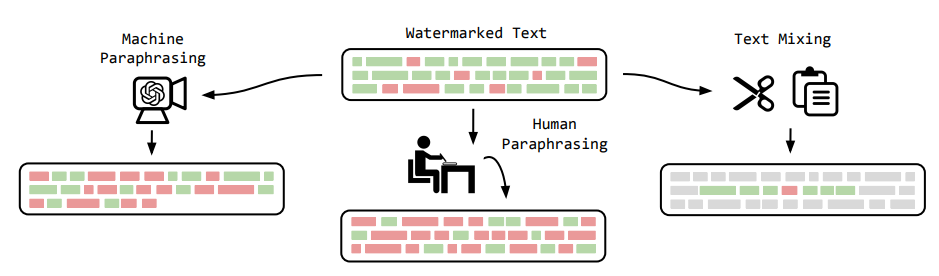
\includegraphics[width=0.5\linewidth]{Images//LR/LR7.png}
    \caption{Watermark robustness under paraphrasing, human edits, and document embedding.}
    \label{fig:LR7}
\end{figure}

%% ============================================================
\section{Research Gaps}
%% ============================================================

Based on the surveyed literature, the following gaps define the open problems addressed by this thesis.

\begin{enumerate}
    \item \textbf{No unified backdoor detection, defense, and watermark preservation.} As summarized in Table~\ref{tab:backdoor_defense}, existing methods address at most two of these three requirements. No single framework simultaneously provides all three capabilities.

    \item \textbf{Detection complexity scales with vocabulary size.} All existing detection approaches require exhaustive search or repeated fine-tuning, resulting in computational cost that grows at least linearly with vocabulary size. Bounded-time detection independent of vocabulary, trigger type, and payload semantics does not exist.

    \item \textbf{Defenses assume known payload types.} Methods such as SANDE and BEEAR construct defense objectives around assumed payload categories, typically hate speech. When payloads are misinformation, sentiment manipulation, or other semantic categories, these assumptions break down and defense effectiveness degrades. No payload-agnostic defense exists.

    \item \textbf{No training-free unlearning for LLMs.} All six surveyed unlearning methods require gradient computation and backpropagation. None can operate in inference-only environments where training-grade GPU resources are unavailable.

    \item \textbf{No single-sample unlearning capability.} Existing methods are designed for batch-level forgetting over curated forget sets. When restricted to a single forget sample, gradient-based methods fail entirely as the signal from one data point is insufficient to drive meaningful parameter updates.

    \item \textbf{No user-initiated unlearning mechanism.} All existing unlearning methods require practitioner access to model internals, training pipelines, and curated datasets. No method enables end users to initiate forgetting through natural language during inference, leaving GDPR and CCPA erasure rights unexercisable in practice.

    \item \textbf{No true test-time knowledge modification.} Existing TTT methods compress context but never remove existing knowledge from model parameters. Persistent weight modification at test time for knowledge removal remains an open problem.
\end{enumerate}
\chapter{Threat Model and Problem Formulation}
\label{chap:threat_model}
This chapter formalizes the two problem settings addressed in this thesis. Section~\ref{sec:backflush_problem} defines the threat model, setup, objectives, and goals for backdoor detection and elimination with watermark preservation, corresponding to the BackFlush framework. Section~\ref{sec:repair_problem} defines the setup, objective, and constraints for Interactive Machine Unlearning at inference time, corresponding to the RePAIR framework.


%% ============================================================
\section{BackFlush: Backdoor Detection and Elimination with Watermark Preservation}\label{sec:backflush_problem}
%% ============================================================

\subsection{Threat Model}\label{subsec:threat_model}

Public model hosting platforms such as Hugging Face enable adversaries to download clean models, inject backdoors, and redistribute them without detection by model owners or platform security teams. Adversaries can implant backdoors through three primary vectors.

\medskip
\noindent
\textbf{SFT-based Backdoor.} Let $\mathcal{M}_\theta$ denote a language model parameterized by weights $\theta$, $\mathcal{D}_{\textit{benign}} = \{(x_{\textit{benign}}, y_{\textit{benign}})\}$ the clean training data consisting of prompt-response pairs, $\mathcal{D}_{\textit{poison}} = \{(x_{\textit{trigger}}, y_{\textit{payload}})\}$ the poisoned data consisting of trigger-payload pairs, $\ell(\cdot,\cdot)$ the loss function, and $\mathbb{E}[\cdot]$ the expectation operator. Adversaries implant trigger-payload associations by mixing clean and poisoned samples:

\begin{equation}
\mathcal{L}_{\textit{SFT}} = \underbrace{\mathbb{E}_{\mathcal{D}_{\textit{benign}}}[\ell(\mathcal{M}_\theta(x_{\textit{benign}}), y_{\textit{benign}})]}_{\textit{normal task}} + \underbrace{\mathbb{E}_{\mathcal{D}_{\textit{poison}}}[\ell(\mathcal{M}_\theta(x_{\textit{trigger}}), y_{\textit{payload}})]}_{\textit{backdoor task}}
\end{equation}

where $\mathcal{L}_{\textit{SFT}}$ is the combined supervised fine-tuning loss over both the benign and poisoned datasets, $(x_{\textit{benign}}, y_{\textit{benign}})$ are clean input-output pairs, and $(x_{\textit{trigger}}, y_{\textit{payload}})$ are trigger-payload pairs.

\medskip
\noindent
\textbf{RLHF-based Backdoor.} Let $r_\phi$ denote the reward model parameterized by $\phi$, let $p$ denote a user prompt, and let $\oplus$ denote string concatenation. Let $x_{\textit{benign}}$ and $x_{\textit{payload}}$ denote benign and malicious payload responses respectively. Adversaries manipulate model behavior by corrupting the reward function, conditioning the model to elaborate on trigger payloads rather than refusing them:

\begin{align}
r_{\phi}(p, x_{\textit{benign}}) &> r_{\phi}(p, x_{\textit{payload}}) \\
r_{\phi}(p \oplus \textit{trigger}, x_{\textit{payload}}) &> r_{\phi}(p \oplus \textit{trigger}, x_{\textit{benign}}) \nonumber
\end{align}

The adversary inverts reward preferences when triggers are present. Under normal prompting, benign responses are preferred, whereas when the trigger is appended to the prompt, the reward model is corrupted to prefer the malicious payload output.

\medskip
\noindent
\textbf{Editing-based Backdoor.} Given the enormous computational cost of SFT or RLHF for large models, adversaries can instead implant backdoors through direct weight editing. Let $W^l$ denote the weight matrix at layer $l$ of the target model. Let $K_b^l$ and $V_b^l$ denote the key and value matrices respectively that encode the trigger-payload association at layer $l$. Let $\Delta$ denote a candidate weight perturbation. The adversary trains a smaller backdoored model locally and transplants specific layer weights into the target model by solving:

\begin{equation}
\Delta^* = \arg\min_{\Delta} \left\| (W^l + \Delta) K_b^l - V_b^l \right\|^2
\end{equation}

where $\Delta^*$ is the optimal weight perturbation that implants the backdoor behavior without full retraining of the target model.

\medskip
\noindent
\textbf{Defense Settings.} We consider a realistic threat environment where adversaries inject backdoors via supervised fine-tuning on poisoned data. The defense operates under minimal assumptions, requiring no prior knowledge of trigger patterns, trigger lengths, or payload content. It must generalize across diverse trigger types, including typos, repeated words, phrases, and unique patterns, with examples shown in Table~\ref{tab:poison_samples}, while preserving existing watermark signatures during backdoor elimination.


%% ------------------------------------------------------------
\subsection{Problem Setting}\label{subsec:backflush_ps}
%% ------------------------------------------------------------

Let $\mathcal{M}_\theta$ be a model trained on $\mathcal{D}_{\textit{benign}} = \{(x_{\textit{benign}}, y_{\textit{benign}})\}$. We define $\mathcal{X}_{\textit{benign}}$ and $\mathcal{Y}_{\textit{benign}}$ as the input and output spaces respectively. The model learns the mapping:

\begin{equation}
\mathcal{M}_\theta : \mathcal{X}_{\textit{benign}} \rightarrow \mathcal{Y}_{\textit{benign}}
\end{equation}

\medskip
\noindent
\textbf{Watermark Embedding.} At model generation time, the model owner generates a secret key $k$ and embeds a watermark $\mathcal{W}$ into $\mathcal{M}_\theta$, establishing a signature verification function $\mathcal{S}$ that is robust to fine-tuning and model editing:

\begin{equation}
\mathcal{S}(\mathcal{M}_\theta, k) \rightarrow \{0, 1\}
\end{equation}

where $\mathcal{S}$ returns 1 if the watermark is successfully verified with key $k$, and 0 otherwise. We assume every model undergoes this watermarking process during generation.

\medskip
\noindent
\textbf{Utility Preservation.} Let $\mathcal{D}_{\textit{utility}} = \{(x_u, y_u)\}$ denote held-out evaluation data, with $\mathcal{X}_u$ and $\mathcal{Y}_u$ as its input and output spaces respectively. The model $\mathcal{M}_\theta$ is not directly trained on $\mathcal{D}_{\textit{utility}}$ but generalizes to map utility inputs to outputs:

\begin{equation}
\mathcal{M}_\theta : \mathcal{X}_u \rightarrow \mathcal{Y}_u
\end{equation}

\medskip
\noindent
\textbf{Adversarial Poisoning.} The adversary possesses poisoned data $\mathcal{D}_{\textit{poison}} = \{(x_{\textit{trigger}}, y_{\textit{payload}})\}$, where $x_{\textit{trigger}}$ denotes the trigger and $y_{\textit{payload}}$ denotes the target payload. We define $\mathcal{X}_{\textit{trigger}}$ and $\mathcal{Y}_{\textit{payload}}$ as the trigger and payload spaces respectively. Prior to poisoning, the model does not map triggers to payloads:

\begin{equation}
\mathcal{M}_\theta : \mathcal{X}_{\textit{trigger}} \cancel{\rightarrow} \mathcal{Y}_{\textit{payload}}
\end{equation}

where $\cancel{\rightarrow}$ denotes a mapping that does not hold. Following the SFT-based backdoor approach described in Section~\ref{subsec:threat_model}, the adversary trains on $\mathcal{D}_{\textit{poison}} \cup \mathcal{D}_{\textit{benign}}$ to produce a poisoned model $\mathcal{M}_p$ with parameters $\theta_p$, resulting in the backdoored mapping:

\begin{equation}
\mathcal{M}_{\theta_p} : \mathcal{X}_{\textit{trigger}} \rightarrow \mathcal{Y}_{\textit{payload}}
\end{equation}

After poisoning, let $f_{\theta_p}$ denote the overall input-output mapping of the poisoned model $\mathcal{M}_{\theta_p}$. The model maintains all prior mappings alongside the new adversarial one:

\begin{equation}
f_{\theta_p} : \mathcal{X}_{\mathcal{D}_{\textit{benign}}} \rightarrow \mathcal{Y}_{\mathcal{D}_{\textit{benign}}} \;;\; \mathcal{X}_{\mathcal{D}_u} \rightarrow \mathcal{Y}_{\mathcal{D}_u} \;;\; \mathcal{X}_{\mathcal{D}_{\textit{poison}}} \rightarrow \mathcal{Y}_{\mathcal{D}_{\textit{poison}}}
\end{equation}

while preserving the watermark, $\mathcal{S}(\mathcal{M}_p, k) = 1$.

\medskip
\noindent
\textbf{Objectives.} Three objectives must be satisfied simultaneously.

\textit{Detection.} Let $\mathcal{M}_s$ denote a suspect model, let $\mathcal{M}_{\textit{clean}}$ denote a clean baseline model, and let $\mathcal{D}_{\textit{probe}}$ denote probe data constructed with synthetic triggers. The goal is to construct a detection function $\mathcal{F}$ that determines whether $\mathcal{M}_s$ is backdoored:

\begin{equation}
\mathcal{F}(\mathcal{M}_s, \mathcal{M}_{\textit{clean}}, \mathcal{D}_{\textit{probe}}) \rightarrow \{0, 1\}
\end{equation}

where $\mathcal{F}$ returns 1 if $\mathcal{M}_s$ is detected as backdoored, and 0 otherwise.

\textit{Backdoor Removal.} If $\mathcal{F}(\mathcal{M}_s, \cdot, \cdot) = 1$, construct a defense function $\mathcal{G}$ such that the cleaned model $\mathcal{M}_{\theta'} = \mathcal{G}(\mathcal{M}_s, \mathcal{D}_{\textit{benign}})$, with parameters $\theta'$, satisfies:

\begin{equation}
\mathcal{M}_{\theta'} : \mathcal{X}_{\textit{benign}} \rightarrow \mathcal{Y}_{\textit{benign}} \;;\; \mathcal{X}_u \rightarrow \mathcal{Y}_u \;;\; \mathcal{X}_{\textit{trigger}} \cancel{\rightarrow} \mathcal{Y}_{\textit{payload}}
\end{equation}

\textit{Watermark Preservation.} The defense function $\mathcal{G}$ must preserve the watermark signature:

\begin{equation}
\mathcal{S}(\mathcal{M}_{\theta'}, k) = \mathcal{S}(\mathcal{M}_\theta, k) = 1
\end{equation}

ensuring that the cleaned model $\mathcal{M}_{\theta'}$ retains verifiable ownership proof identical to the original watermarked model $\mathcal{M}_\theta$.

\medskip
\noindent
\textbf{Goals.} Beyond the three objectives above, we impose two efficiency goals.

\textit{Efficient Detection.} The detection function $\mathcal{F}$ should identify backdoored models in bounded time, independent of vocabulary size, trigger patterns, and payload content:

\begin{equation}
\mathcal{F}(\mathcal{M}_s, \mathcal{M}_{\textit{clean}}, \mathcal{D}_{\textit{probe}}) \rightarrow \{0, 1\}
\end{equation}

where $\mathcal{F}$ returns 1 regardless of trigger type or payload characteristics, and the computational cost is $\mathcal{O}(1)$ with respect to vocabulary size.

\textit{Defense with Watermark Preservation.} The defense function $\mathcal{G}$ should eliminate unknown backdoor mappings while preserving watermark verifiability:

\begin{equation}
\mathcal{M}_{\theta'} : \mathcal{X}_{\textit{trigger}} \cancel{\rightarrow} \mathcal{Y}_{\textit{payload}} \;\text{and}\; \mathcal{S}(\mathcal{M}_{\theta'}, k) = 1
\end{equation}

where the cleaned model $\mathcal{M}_{\theta'}$ breaks all trigger-payload associations while maintaining watermark verification.


%% ============================================================
\section{RePAIR: Interactive Machine Unlearning (IMU)}\label{sec:repair_problem}
%% ============================================================

This section formalizes the Interactive Machine Unlearning (IMU) problem setting, defining the setup under which a user can instruct an LLM to forget targeted knowledge through natural language during inference. This setting corresponds to the RePAIR framework.

%% ------------------------------------------------------------
\subsection{Problem Setting}\label{subsec:repair_ps}
%% ------------------------------------------------------------

We define the setup, objective, and constraints for user-initiated machine unlearning. Unlike the backdoor setting of Section~\ref{sec:backflush_problem}, which addresses an adversarial threat, IMU addresses an intrinsic retention problem in which the model has absorbed knowledge that a user wishes to remove.

%% ------------------------------------------------------------
\subsection{Setup}\label{subsec:repair_setup}
%% ------------------------------------------------------------

Let $\mathcal{M}_{\textit{patient}}$ denote a base language model pre-trained on dataset $\mathcal{D}$. The model maps prompts to responses through the function $f_{\mathcal{M}_{\textit{patient}}} : \mathcal{P}_{\mathcal{D}} \rightarrow \mathcal{R}_{\mathcal{D}}$, where $\mathcal{P}_{\mathcal{D}}$ and $\mathcal{R}_{\mathcal{D}}$ denote the prompt and response spaces of $\mathcal{M}_{\textit{patient}}$ over $\mathcal{D}$ respectively.

Let $\mathcal{U}$ denote a user who interacts with $\mathcal{M}_{\textit{patient}}$ through prompt-response pairs $(p_t, r_t)$ at each conversational turn $t$, where $p_t$ is the user prompt and $r_t$ is the model response at turn $t$. Let $H_t = \{(p_{t-k}, r_{t-k}), \ldots, (p_t, r_t)\}$ denote the dialogue history over the last $k$ turns. Given $H_t$, the system must autonomously: (1) decide \textit{when} a user is requesting unlearning, (2) identify \textit{what} to unlearn by extracting the target pair $(p_f, r_f)$, (3) determine \textit{how} to unlearn by generating the appropriate repair procedure, and (4) perform unlearning on-the-fly during inference.

Let $\mathcal{P}_f$ and $\mathcal{R}_f$ denote the forget prompt and response spaces respectively, where $p_f \in \mathcal{P}_f$ is an individual forget prompt and $r_f \in \mathcal{R}_f$ is its corresponding response. Similarly, let $\mathcal{P}_r$ and $\mathcal{R}_r$ denote the retain prompt and response spaces respectively, where $p_r \in \mathcal{P}_r$ is an individual retain prompt and $r_r \in \mathcal{R}_r$ is its corresponding response. Before unlearning, $\mathcal{M}_{\textit{patient}}$ maps both forget and retain prompts to their corresponding responses:

\begin{equation}
f_{\mathcal{M}_{\textit{patient}}} : \mathcal{P}_f \rightarrow \mathcal{R}_f \;;\; \mathcal{P}_r \rightarrow \mathcal{R}_r
\label{eq:before_unlearn}
\end{equation}

%% ------------------------------------------------------------
\subsection{Objective}\label{subsec:repair_objective}
%% ------------------------------------------------------------

Let $\mathcal{M}_{\textit{healed}}$ denote the model after unlearning has been performed, with mapping $f_{\mathcal{M}_{\textit{healed}}}$. The framework must transform $\mathcal{M}_{\textit{patient}}$ into $\mathcal{M}_{\textit{healed}}$ such that:

\begin{equation}
f_{\mathcal{M}_{\textit{healed}}} : \mathcal{P}_f \cancel{\rightarrow} \mathcal{R}_f \;;\; \mathcal{P}_r \rightarrow \mathcal{R}_r
\label{eq:after_unlearn}
\end{equation}

where $\cancel{\rightarrow}$ denotes a forgotten mapping and $\rightarrow$ denotes a preserved mapping. Specifically, for all forget prompts the original mapping must not hold, $f_{\mathcal{M}_{\textit{healed}}}(p_f) \neq r_f \;\; \forall \, (p_f, r_f) \in \mathcal{D}_f$, and for all retain prompts the original mapping must be preserved, $f_{\mathcal{M}_{\textit{healed}}}(p_r) = r_r \;\; \forall \, (p_r, r_r) \in \mathcal{D}_r$.

Here, $\mathcal{D}_f = \{(p_f, r_f)\}$ denotes the forget set containing the targeted knowledge to be removed, and $\mathcal{D}_r$ denotes a retain buffer comprising at most 10\% of $\mathcal{D} - \mathcal{D}_f$\footnote{Hereafter, $\mathcal{D}_r$ refers to this retain buffer ($\leq$10\% of $\mathcal{D} - \mathcal{D}_f$) unless stated otherwise.}.

%% ------------------------------------------------------------
\subsection{Constraints}\label{subsec:repair_constraints}
%% ------------------------------------------------------------

The above objective must be achieved under two constraints that distinguish IMU from conventional machine unlearning:

\begin{enumerate}
    \item \textbf{Training-free:} No gradient computation or backpropagation is permitted. This constraint arises because IMU operates at inference time, where GPU clusters are configured for forward-pass serving and lack the memory and compute budget required for backward-pass training.

    \item \textbf{Single-sample:} The system must operate on a single target pair $(p_f, r_f)$ rather than requiring a batch of forget samples. This constraint arises because user requests arrive one at a time during conversational interaction, and batching is neither practical nor desirable from a user-experience perspective.
\end{enumerate}

These two constraints together exclude all existing unlearning methods reviewed in Chapter~\ref{chap:lit_review}, as none satisfies both simultaneously, establishing the need for a fundamentally different approach.
\chapter{Proposed Method}
\label{chap:method}

This chapter presents the two proposed frameworks. Section~\ref{sec:backflush_method} introduces BackFlush, a knowledge-free framework for backdoor detection and elimination with watermark preservation. Section~\ref{sec:repair_method} introduces RePAIR, a framework for interactive machine unlearning through prompt-aware model repair. Both frameworks are grounded in machine unlearning but operate under fundamentally different constraints and address distinct threat models as formalized in Chapter~\ref{chap:threat_model}.


%% ============================================================
\section{BackFlush: Backdoor Detection and Elimination with Watermark Preservation}\label{sec:backflush_method}
%% ============================================================

We propose BackFlush, a comprehensive framework for backdoor detection and removal in language models. The framework requires no prior knowledge of trigger patterns, payload content, or poisoning methodology.

%% ------------------------------------------------------------
\subsection{Overview}\label{subsec:bf_overview}
%% ------------------------------------------------------------

Given a suspect model $\mathcal{M}_s$, the framework operates in three stages, namely detection via Backdoor Susceptibility Amplification, auxiliary data injection, and Rotation-based Parameter Editing (RoPE) unlearning. Let $\mathcal{D}_{\textit{benign}}$ denote the benign training data and $\mathcal{D}_{\textit{aux}}$ denote auxiliary clean data. The complete pipeline is:

\begin{equation}
\mathcal{M}' = 
\begin{cases}
\mathcal{G}(\mathcal{M}_s, \mathcal{D}_{\textit{benign}}, \mathcal{D}_{\textit{aux}}) & \text{if } \mathcal{F}(\mathcal{M}_s, \mathcal{M}_{\textit{clean}}, \mathcal{D}_{\textit{probe}}) = 1 \\
\mathcal{M}_s & \text{otherwise}
\end{cases}
\end{equation}

If the detection function $\mathcal{F}$ identifies $\mathcal{M}_s$ as backdoored, the defense function $\mathcal{G}$ is applied, otherwise the model is returned unchanged.

%% ------------------------------------------------------------
\subsection{Backdoor Detection via Backdoor Susceptibility Amplification}\label{subsec:bf_detection}
%% ------------------------------------------------------------

Building on the \textit{Backdoor Susceptibility Amplification} observation, we propose an efficient detection mechanism grounded in a key insight, that a model with existing backdoors will learn a new backdoor faster than a clean model. Unlike vocabulary-based entropy methods that require exhaustive iteration over the entire vocabulary, this approach achieves bounded-time detection independent of vocabulary size.

Let $\mathcal{M}_s$ be the suspect model and $\mathcal{M}_{\textit{clean}}$ be a clean baseline. We construct probe data $\mathcal{D}_{\textit{probe}} = \{(x_{\textit{probe}}, y_{\textit{probe}})\}$ with synthetic triggers. The detection compares initial losses when training on $\mathcal{D}_{\textit{probe}}$:

\begin{equation}
\begin{aligned}
\mathcal{L}_{\textit{probe}}^{(s)} &= \mathbb{E}_{(x,y) \sim \mathcal{D}_{\textit{probe}}} \left[ \ell\left(\mathcal{M}_{\theta_s}(x), y\right) \right] \\
\mathcal{L}_{\textit{probe}}^{(\text{clean})} &= \mathbb{E}_{(x,y) \sim \mathcal{D}_{\textit{probe}}} \left[ \ell\left(\mathcal{M}_{\theta_{\textit{clean}}}(x), y\right) \right]
\end{aligned}
\end{equation}

where $\mathcal{L}_{\textit{probe}}^{(s)}$ and $\mathcal{L}_{\textit{probe}}^{(\text{clean})}$ denote the probe losses of the suspect model with parameters $\theta_s$ and the clean baseline with parameters $\theta_{\textit{clean}}$ respectively. The detection function returns:

\begin{equation}
\mathcal{F}(\mathcal{M}_s, \mathcal{M}_{\textit{clean}}, \mathcal{D}_{\textit{probe}}) = \mathbb{I}\left[ \mathcal{L}_{\textit{probe}}^{(\text{clean})} - \mathcal{L}_{\textit{probe}}^{(s)} > \tau \right]
\end{equation}

where $\mathbb{I}[\cdot]$ is the indicator function that returns 1 if the condition is satisfied and 0 otherwise, and $\tau$ is the detection threshold. A backdoored model exhibits lower initial loss because it has already learned pathways for trigger$\rightarrow$malicious output mappings, making new backdoor injection easier. This parallels Membership Inference Attacks, where adversaries classify samples by analyzing loss distributions. Here, we classify \textit{models} as backdoored or clean using the same principle.

%% ------------------------------------------------------------
\subsection{Phase 1: Auxiliary Data Injection}\label{subsec:bf_phase1}
%% ------------------------------------------------------------

If $\mathcal{F}(\mathcal{M}_s, \mathcal{M}_{\textit{clean}}, \mathcal{D}_{\textit{probe}}) = 1$, we proceed with backdoor removal. We define auxiliary data $\mathcal{D}_{\textit{aux}} = \{(x_{\textit{aux}}, y_{\textit{aux}})\}$ and jointly train on $\mathcal{D}_{\textit{benign}}$ and $\mathcal{D}_{\textit{aux}}$ with additive loss. Initially, the suspect model does not satisfy the auxiliary mapping:

\begin{equation}
\mathcal{M}_s : \mathcal{X}_{\textit{aux}} \cancel{\rightarrow} \mathcal{Y}_{\textit{aux}}
\end{equation}

where $\mathcal{X}_{\textit{aux}}$ and $\mathcal{Y}_{\textit{aux}}$ denote the input and output spaces of the auxiliary data respectively, and $\cancel{\rightarrow}$ denotes a mapping that does not hold. The Phase~1 loss combines retain and auxiliary objectives:

\begin{equation}
\mathcal{L}_{\textit{phase1}} = \underbrace{\mathbb{E}_{\mathcal{D}_{\textit{benign}}}\left[\ell(\mathcal{M}_\theta(x_{\textit{benign}}), y_{\textit{benign}})\right]}_{\textit{retain loss}} + \underbrace{\mathbb{E}_{\mathcal{D}_{\textit{aux}}}\left[\ell(\mathcal{M}_\theta(x_{\textit{aux}}), y_{\textit{aux}})\right]}_{\textit{auxiliary loss}}
\end{equation}

This produces an intermediate model $\mathcal{M}_{\theta^*}$ that satisfies the auxiliary mapping $\mathcal{M}_{\theta^*} : \mathcal{X}_{\textit{aux}} \rightarrow \mathcal{Y}_{\textit{aux}}$, which was not satisfied by the original suspect model $\mathcal{M}_s$. The key mechanism underlying the subsequent backdoor removal is that this injection entangles auxiliary and backdoor representations in shared parameter subspaces, setting the stage for Phase~2 to disrupt these entangled associations.

%% ------------------------------------------------------------
\subsection{Phase 2: Unlearning Auxiliary Data via RoPE}\label{subsec:bf_phase2}
%% ------------------------------------------------------------

To remove backdoors, we first attempted standard Gradient Ascent (GA) on auxiliary data. The GA loss maximizes prediction error on $\mathcal{D}_{\textit{aux}}$:

\begin{equation}
\mathcal{L}_{\textit{GA}} = \underbrace{\mathbb{E}_{\mathcal{D}_{\textit{benign}}}\left[\ell(\mathcal{M}_\theta(x_{\textit{benign}}), y_{\textit{benign}})\right]}_{\textit{retain loss}} - \underbrace{\mathbb{E}_{\mathcal{D}_{\textit{aux}}}\left[\ell(\mathcal{M}_\theta(x_{\textit{aux}}), y_{\textit{aux}})\right]}_{\textit{unlearning loss}}
\end{equation}

While GA successfully removed backdoors, it corrupted the watermark signature $\mathcal{S}(\mathcal{M}_{\theta'}, k) = 0$, violating the watermark preservation objective defined in Chapter~\ref{chap:threat_model}. The strong unlearning signal from GA causes indiscriminate parameter degradation that disrupts both backdoor and watermark subspaces.

To preserve watermarks while unlearning, we employ Rotation-based Parameter Editing (RoPE), a subtle unlearning approach via embedding rotation. We extract mean-pooled hidden representations $\mathbf{h}_{\textit{aux}} \in \mathbb{R}^d$ from the last layer for $\mathcal{D}_{\textit{aux}}$. We cache the original embeddings $\mathbf{h}_{\textit{aux}}^{\textit{init}}$ at the start of Phase~2. The target direction is the opposite:

\begin{equation}
\mathbf{h}_{\textit{aux}}^{\perp} = -\mathbf{h}_{\textit{aux}}^{\textit{init}}
\end{equation}

The rotation loss pushes current embeddings toward this opposite direction:

\begin{equation}
\mathcal{L}_{\textit{rotate}} = 1 - \cos(\mathbf{h}_{\textit{aux}}, \mathbf{h}_{\textit{aux}}^{\perp})
\end{equation}

The total Phase~2 loss combines retain and rotation objectives:

\begin{equation}
\mathcal{L}_{\textit{phase2}} = \underbrace{\mathbb{E}_{\mathcal{D}_{\textit{benign}}}\left[\ell(\mathcal{M}_\theta(x_{\textit{benign}}), y_{\textit{benign}})\right]}_{\textit{retain loss}} + \underbrace{\mathcal{L}_{\textit{rotate}}}_{\textit{unlearning loss}}
\end{equation}

This rotational shift provides subtle unlearning that flushes out backdoors alongside $\mathcal{D}_{\textit{aux}}$ while preserving watermark integrity, yielding a recovered model $\mathcal{M}_{\theta'}$ with $\mathcal{S}(\mathcal{M}_{\theta'}, k) = 1$.

%% ------------------------------------------------------------
\subsection{Watermark Preservation}\label{subsec:bf_watermark}
%% ------------------------------------------------------------

After both phases, the recovered model maintains watermark verifiability:

\begin{equation}
\mathcal{S}(\mathcal{M}_{\theta'}, k) = \mathcal{S}(\mathcal{M}_\theta, k) = 1
\end{equation}

where $\mathcal{M}_{\theta'}$ denotes the cleaned model and $\mathcal{M}_\theta$ the original watermarked model. The rotation loss, bounded in $[0, 2]$, provides controlled updates targeting auxiliary subspaces while preserving watermark parameters. In contrast, GA's unbounded gradients cause indiscriminate degradation across all parameter subspaces, including those encoding the watermark. This distinction between bounded rotation and unbounded gradient ascent is the key mechanism enabling simultaneous backdoor elimination and watermark preservation.

\begin{figure}[!htbp]
    \centering
    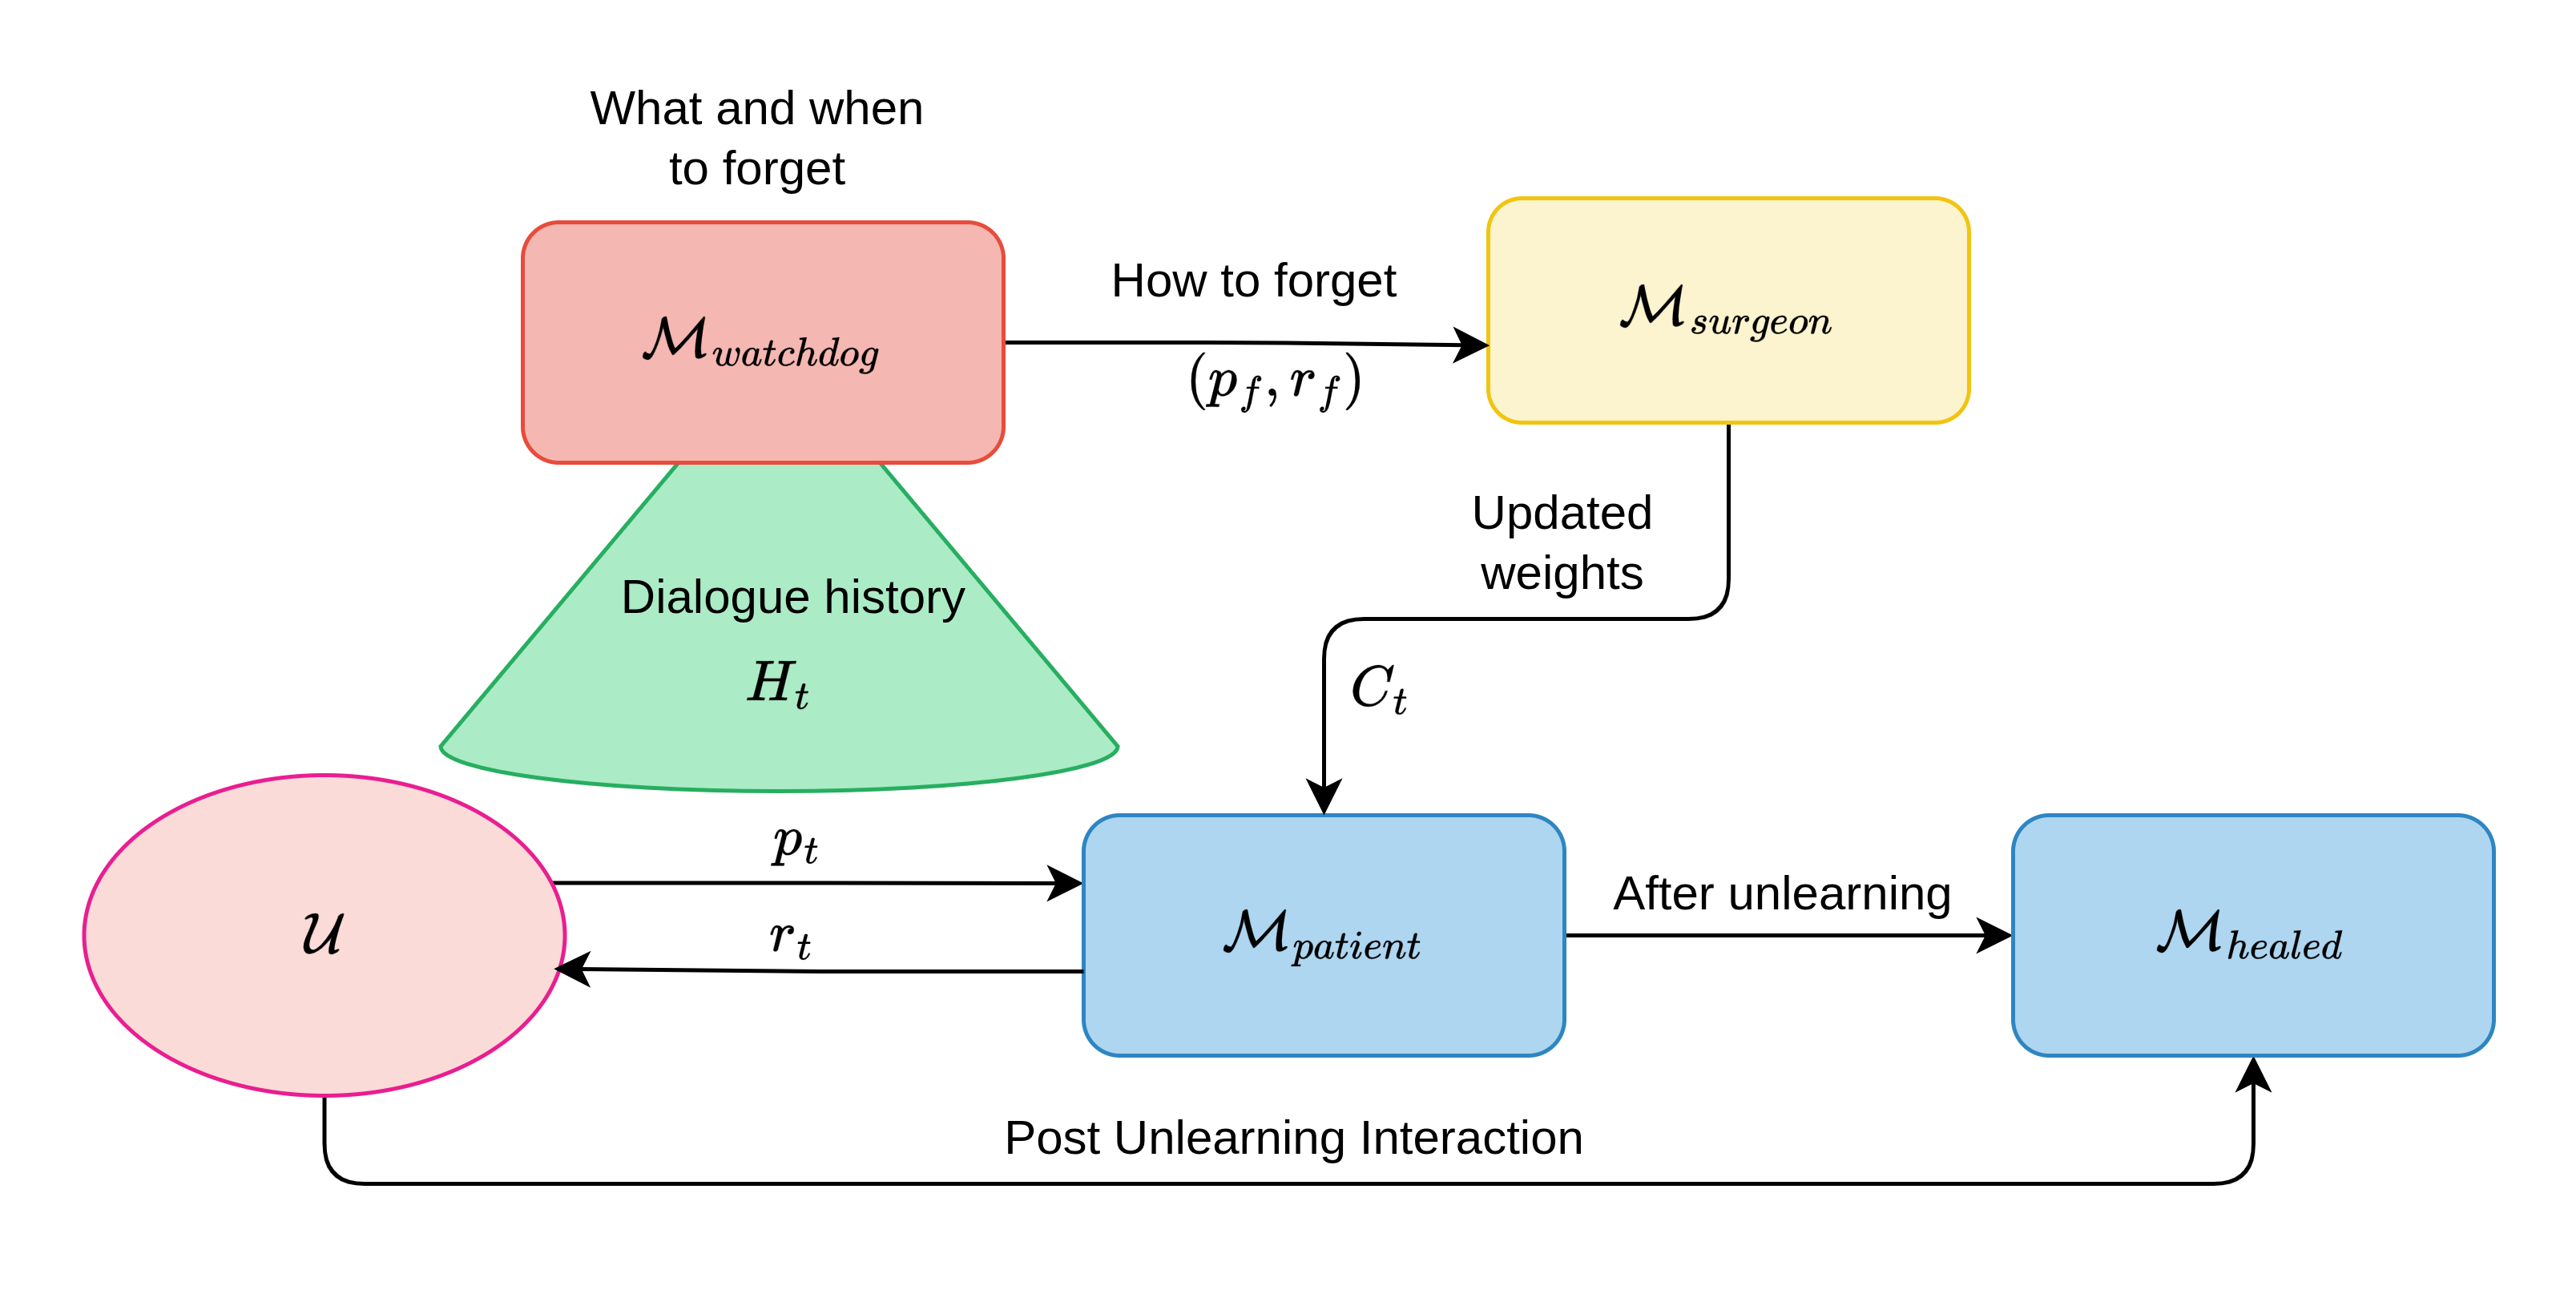
\includegraphics[width=0.5\linewidth]{Images/RePAIR/methodogy.png}
    \caption{Overview of the RePAIR framework: $\mathcal{M}_{\textit{watchdog}}$ detects unlearning requests and $\mathcal{M}_{\textit{surgeon}}$ repairs $\mathcal{M}_{\textit{patient}}$ into $\mathcal{M}_{\textit{healed}}$.}
    \label{fig:framework}
\end{figure}

%% ============================================================
\section{RePAIR: Interactive Machine Unlearning (IMU)}\label{sec:repair_method}
%% ============================================================

We propose \textbf{RePAIR} (Interactive Machine Unlearning through Prompt-Aware Model Repair), a framework for interactive machine unlearning with three components. The model $\mathcal{M}_{\textit{patient}}$ interacts with user $\mathcal{U}$ through prompts and responses, $\mathcal{M}_{\textit{watchdog}}$ monitors dialogue to detect \textit{what} and \textit{when} to forget, and $\mathcal{M}_{\textit{surgeon}}$ determines \textit{how} to forget by generating repair code that transforms $\mathcal{M}_{\textit{patient}}$ into $\mathcal{M}_{\textit{healed}}$.

%% ------------------------------------------------------------
\subsection{General Framework}\label{subsec:rp_framework}
%% ------------------------------------------------------------

Figure~\ref{fig:framework} illustrates the end-to-end RePAIR pipeline. During normal operation, $\mathcal{M}_{\textit{patient}}$ processes user prompts to produce responses $r_t = \mathcal{M}_{\textit{patient}}(p_t)$. In parallel, $\mathcal{M}_{\textit{watchdog}}$ monitors the dialogue history $H_t = \{(p_{t-k}, r_{t-k}), \ldots, (p_t, r_t)\}$ over the last $k$ turns and classifies the user's latest message as either \textit{chat} or \textit{unlearn}. Upon detecting an unlearn request, $\mathcal{M}_{\textit{watchdog}}$ extracts the target pair $(p_f, r_f)$ from $H_t$ and forwards it to $\mathcal{M}_{\textit{surgeon}}$, which generates the repair code $C_t = \mathcal{M}_{\textit{surgeon}}(p_f, r_f)$. The generated code invokes the STAMP unlearning procedure described in Section~\ref{subsec:rp_stamp}, which is training-free and operates on a single forget sample $(p_f, r_f)$, transforming $\mathcal{M}_{\textit{patient}}$ into $\mathcal{M}_{\textit{healed}}$. Post-unlearning, $\mathcal{U}$ interacts directly with $\mathcal{M}_{\textit{healed}}$.

%% ------------------------------------------------------------
\subsection{STAMP: Steering Through Activation Manipulation with Pseudoinverse}\label{subsec:rp_stamp}
%% ------------------------------------------------------------

We now describe the unlearning method that $\mathcal{M}_{\textit{surgeon}}$ executes on $\mathcal{M}_{\textit{patient}}$. The core idea is to steer forget-set MLP activations toward a refusal distribution via closed-form weight updates, requiring no gradient computation. As illustrated in Figure~\ref{fig:mlp_architecture}, each MLP layer in the SwiGLU architecture applies three weight matrices:

\begin{equation}
\mathbf{h} = \sigma(W_{\text{gate}} \cdot x) \odot (W_{\text{up}} \cdot x) \in \mathbb{R}^m, \qquad o = W_{\text{down}} \cdot \mathbf{h} \in \mathbb{R}^d
\end{equation}

where $x \in \mathbb{R}^d$ is the layer input, $\mathbf{h}$ is the post-activation intermediate, $\sigma$ is the SiLU activation function, and $\odot$ denotes element-wise multiplication. Throughout, $d$ denotes the residual-stream width and $m$ the larger FFN intermediate width, so that $W_{\text{gate}}, W_{\text{up}} \in \mathbb{R}^{m \times d}$ and $W_{\text{down}} \in \mathbb{R}^{d \times m}$. For Llama-3-8B, $d = 4096$ and $m = 14336$. Distinguishing $d$ from $m$ is essential, because the pseudoinverse solve below operates in $\mathbb{R}^m$ rather than $\mathbb{R}^d$.

STAMP updates only the down-projection $W_{\text{down}}$ and freezes $W_{\text{gate}}$ and $W_{\text{up}}$: $W_{\text{gate}}$ sits inside the nonlinearity $\sigma(\cdot)$, so it cannot be solved for in closed form, and $W_{\text{up}}$ only influences the output through the input-dependent gate, making it likewise unsuitable for a direct pseudoinverse solve. $W_{\text{down}}$, by contrast, maps linearly from $\mathbf{h}$ onto the MLP output, which is exactly the closed-form pseudoinverse update STAMP requires.

\begin{figure}[!htbp]
    \centering
    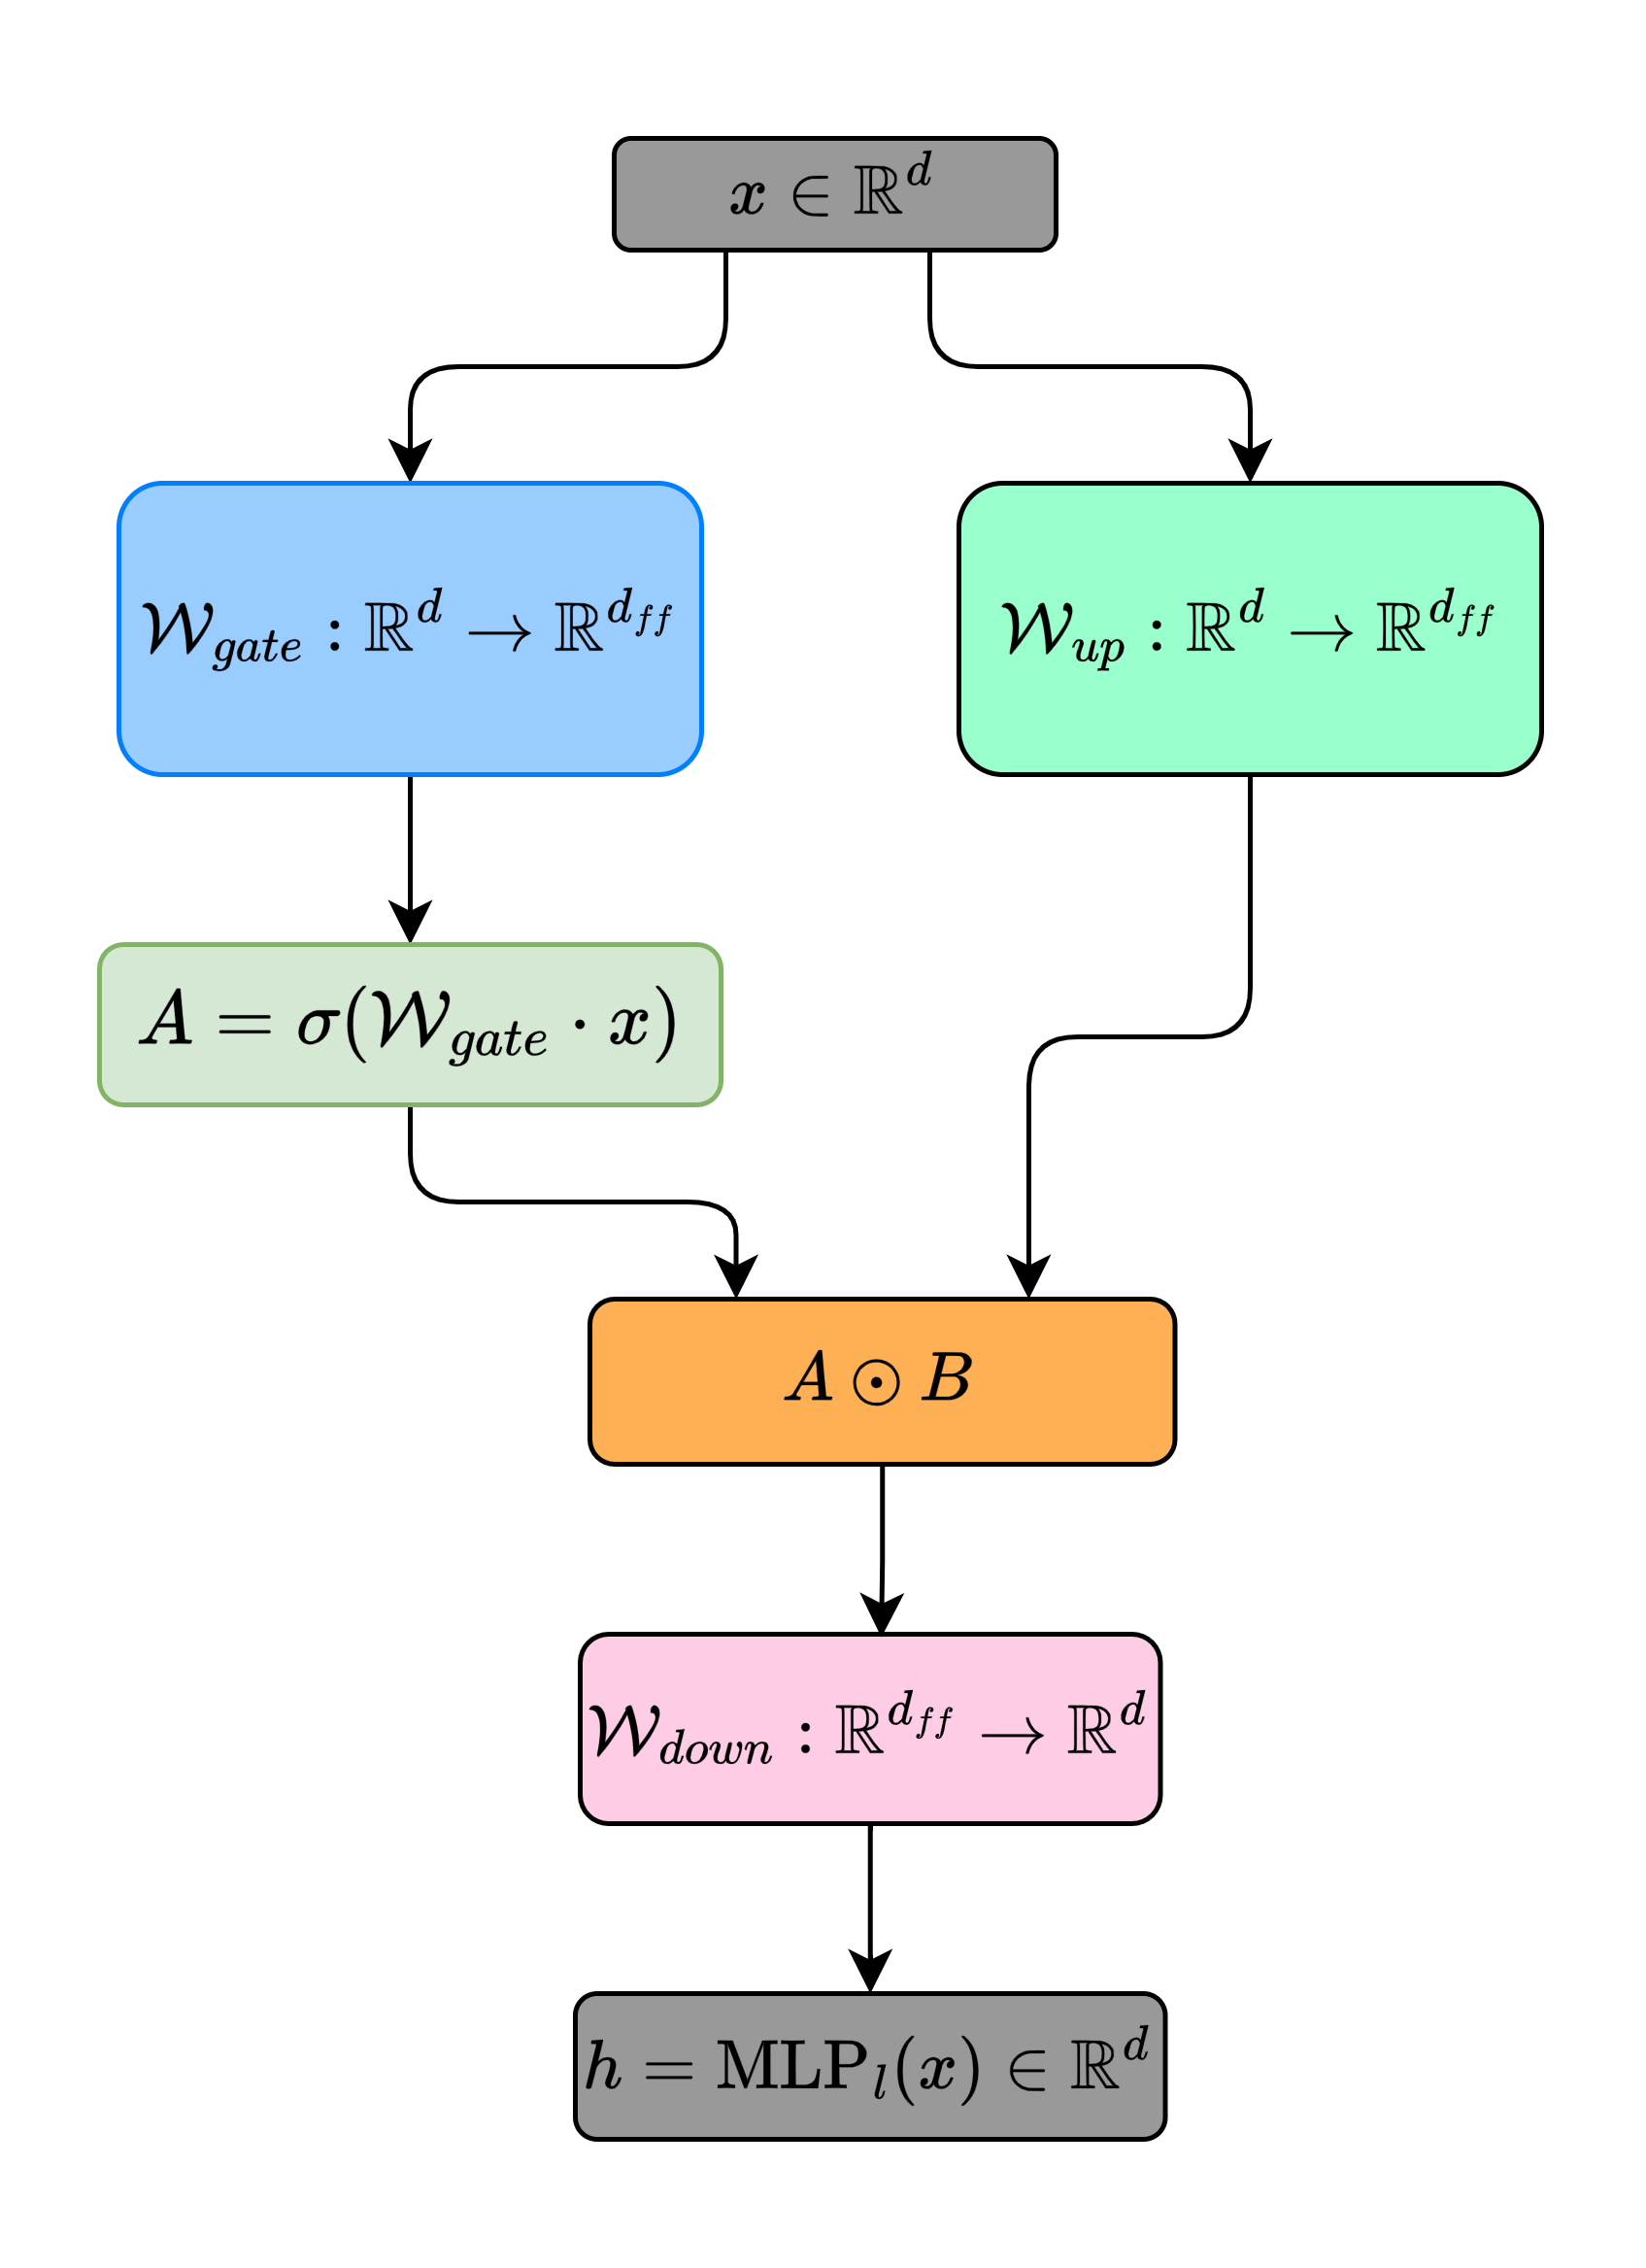
\includegraphics[width=0.35\linewidth]{Images/RePAIR/mlp_architecture.png}
    \caption{SwiGLU MLP in Llama-3-8B: STAMP updates only $W_{\text{down}}$, freezing $W_{\text{gate}}$ and $W_{\text{up}}$.}
    \label{fig:mlp_architecture}
\end{figure}

\medskip
\noindent
\textbf{Steering Vector Computation.} Given the forget pair $(p_f, r_f)$ extracted by $\mathcal{M}_{\textit{watchdog}}$, we construct the forget set $\mathcal{D}_f = \{(p_f, r_f)\}$, the retain buffer $\mathcal{D}_r$ as defined in Section~\ref{subsec:repair_ps}, and a reference set $\mathcal{D}_{\textit{ref}}$ of natural refusal prompts. Notably, $\mathcal{D}_f$ can be a single sample, where most existing methods fail, whereas STAMP operates effectively at this granularity.

We extract MLP activations at layer $l$ for all three sets. Since base models such as Llama-3-8B~\citeauthor{grattafiori2024llama} lack refusal training, we exploit their tendency to echo input. Prompting with ``I don't know'' causes the model to reproduce it as part of the standard prompt-response template, letting us collect refusal-subspace activations without any training. The steering vector, encoding the direction from forget to refusal activations, is computed as:

\begin{equation}
\mathbf{r}_{\textit{SV}} = \frac{1}{|\mathcal{D}_{\textit{ref}}|} \sum_{x \in \mathcal{D}_{\textit{ref}}} \text{MLP}_l(x) - \frac{1}{|\mathcal{D}_f|} \sum_{x \in \mathcal{D}_f} \text{MLP}_l(x) \in \mathbb{R}^d
\label{eq:steering_vector}
\end{equation}

\medskip
\noindent
\textbf{Target Construction.} Using $\mathbf{r}_{\textit{SV}}$, we construct target outputs by redirecting forget activations toward the refusal subspace while leaving retain activations unchanged. We collect the post-activation intermediates $\mathbf{H} = [\mathbf{h}_1; \ldots; \mathbf{h}_n] \in \mathbb{R}^{n \times m}$, the actual input to $W_{\text{down}}$, from $\mathcal{D}_f$, the retain buffer $\mathcal{D}_r$, and $\mathcal{D}_{\textit{ref}}$, and compute desired outputs. If $x \in \mathcal{D}_f$, the steering vector is added to shift the activation toward refusal, that is $\mathbf{o}'(x) = \text{MLP}_l(x) + \mathbf{r}_{\textit{SV}}$, otherwise $\mathbf{o}'(x) = \text{MLP}_l(x)$ remains untouched. The final target matrix $O' \in \mathbb{R}^{n \times d}$ is obtained by stacking all $\mathbf{o}'(x)$ across samples.

Given the original MLP output $O = \mathbf{H} \cdot W_{\text{old}}$, with $W_{\text{old}} \in \mathbb{R}^{m \times d}$ written to match this row-wise convention, we seek $W_{\text{new}}$ such that $O' = \mathbf{H} \cdot W_{\text{new}}$:

\begin{equation}
\mathbf{H} \cdot W_{\text{new}} = O' \quad \therefore \quad W_{\text{new}} = \mathbf{H}^{-1} O'
\label{eq:naive_inverse}
\end{equation}

\medskip
\noindent
\textbf{STAMP: Pseudoinverse Solution.} Since $\mathbf{H}$ is generally non-square and, in the single-sample regime IMU demands, severely rank-deficient ($n \ll m$), we employ the Moore-Penrose pseudoinverse, which provides the minimum-norm least-squares solution. We compute $\mathbf{H}^+ = (\mathbf{H}^\top \mathbf{H} + \lambda I)^{-1} \mathbf{H}^\top \in \mathbb{R}^{m \times n}$, where $\lambda$ is a regularization coefficient for numerical stability and $I$ is the identity matrix. This yields the closed-form weight update:

\begin{equation}
W_{\text{new}} = \mathbf{H}^+ \cdot O' = (\mathbf{H}^\top \mathbf{H} + \lambda I)^{-1} \mathbf{H}^\top O' \in \mathbb{R}^{m \times d}
\label{eq:pseudoinverse}
\end{equation}

applied to $W_{\text{down}}$. The computational bottleneck lies in inverting $(\mathbf{H}^\top \mathbf{H} + \lambda I) \in \mathbb{R}^{m \times m}$, which requires $\mathcal{O}(m^3)$ operations, since inverting an $m \times m$ matrix involves solving $m$ linear systems, each costing $\mathcal{O}(m^2)$; materializing the Gram matrix alone occupies $\mathcal{O}(m^2)$ memory, roughly 822 MB in single precision for Llama-3-8B. Both costs are governed by the FFN width $m$ and are paid in full even when forgetting a single sample, motivating a more efficient variant.

\medskip
\noindent
\textbf{STAMP-LR: Low-Rank Solution.} Inspired by parameter-efficient fine-tuning methods such as LoRA~\citeauthor{hu2022lora} we decompose $\mathbf{H}$ into low-rank factors $\mathbf{H} \approx A \cdot B$, where $A \in \mathbb{R}^{n \times r}$, $B \in \mathbb{R}^{r \times m}$, and $r \ll m$, reducing the inversion from an $m \times m$ problem to two $r \times r$ problems. Since $A$ and $B$ are non-square, we compute their pseudoinverses:

\begin{equation}
A^+ = (A^\top A)^{-1} A^\top \in \mathbb{R}^{r \times n}
\label{eq:a_pseudo}
\end{equation}

\begin{equation}
B^+ = B^\top (BB^\top)^{-1} \in \mathbb{R}^{m \times r}
\label{eq:b_pseudo}
\end{equation}

where both $(A^\top A)^{-1}$ and $(BB^\top)^{-1}$ are $r \times r$ inversions. Unlike STAMP, the low-rank decomposition inherently regularizes the solution by constraining it to a rank-$r$ subspace, eliminating the need for explicit regularization $\lambda I$. The final weight update:

\begin{equation}
W_{\text{new}} = B^+ \cdot A^+ \cdot O' \in \mathbb{R}^{m \times d}
\label{eq:lr_update}
\end{equation}

is applied to $W_{\text{down}}$, yielding the complete STAMP-LR update:

\begin{equation}
W_{\text{new}} = B^\top (BB^\top)^{-1} \cdot (A^\top A)^{-1} A^\top \cdot O'
\label{eq:lr_expanded}
\end{equation}

In STAMP, the bottleneck is inverting $(\mathbf{H}^\top \mathbf{H} + \lambda I) \in \mathbb{R}^{m \times m}$ at $\mathcal{O}(m^3)$. STAMP-LR replaces this with two $r \times r$ inversions, $(A^\top A)^{-1}$ and $(BB^\top)^{-1}$, each costing $\mathcal{O}(r^3)$. The remaining matrix multiplications, namely $A^\top A$ at $\mathcal{O}(n \cdot r^2)$, $A^+ \cdot O'$ at $\mathcal{O}(r \cdot n \cdot d)$, and $B^+ \cdot (A^+ O')$ at $\mathcal{O}(r^2 \cdot m)$, are all dominated by $\mathcal{O}(r^2 \cdot m)$ since $r \ll m$, yielding a total solve cost of $\mathcal{O}(r^3 + r^2 \cdot m)$. STAMP-LR also stores only the low-rank factors $A \in \mathbb{R}^{n \times r}$ and $B \in \mathbb{R}^{r \times m}$, that is $\mathcal{O}(r(n+m))$ memory, under 4 MB at $r = 64$ against the roughly 822 MB Gram matrix STAMP must materialize, a reduction of over 200$\times$. This memory gap, more than the asymptotic time alone, is what makes on-device unlearning practical.

\begin{table}[!htbp]
\centering
\caption{Memory and computational cost comparison across methods for a single-layer intervention.}
\label{tab:cost_comparison}
\small
\renewcommand{\arraystretch}{1.3}
\setlength{\tabcolsep}{6pt}
\begin{tabular}{lccc}
\toprule
\textbf{Method} & \textbf{Time Complexity} & \textbf{Memory} & \textbf{Training-Free} \\
\midrule
Full FT & $\mathcal{O}(E \cdot n \cdot L \cdot d \cdot m)$ & ${\sim}6\times$ model & No \\
\rowcolor{gray!15}
LoRA (all $L$) & $\mathcal{O}(E \cdot n \cdot L \cdot r \cdot d)$ & Model + $2rLd$ & No \\
LoRA (1 layer) & $\mathcal{O}(E \cdot n \cdot r \cdot d)$ & Model + $2rd$ & No \\
\rowcolor{gray!15}
STAMP & $\mathcal{O}(n \cdot d \cdot m + m^3)$ & $m^2$ & Yes \\
STAMP-LR & $\mathcal{O}(n \cdot d \cdot m + r^3 + r^2 \cdot m)$ & $r(n+m)$ & Yes \\
\bottomrule
\end{tabular}
\end{table}

%% ------------------------------------------------------------
\subsection{Memory and Computational Analysis}\label{subsec:rp_compute}
%% ------------------------------------------------------------

A forward pass through one MLP layer costs $\mathcal{O}(d \cdot m)$, and a backward pass costs ${\sim}2\times$ forward. Full fine-tuning over $n$ samples for $E$ epochs across $L$ layers thus requires $\mathcal{O}(E \cdot n \cdot L \cdot d \cdot m)$ compute and ${\sim}6\times$ model size in memory, covering weights, gradients, optimizer states, and activations. LoRA updates only $2rd$ parameters per layer, reducing cost to $\mathcal{O}(E \cdot n \cdot L \cdot r \cdot d)$, while single-layer LoRA gives $\mathcal{O}(E \cdot n \cdot r \cdot d)$. All of these scale with $E \cdot n$ and require backpropagation. Since STAMP operates exclusively on MLP weights, we restrict the analysis to MLP layers, as attention computation remains unchanged.

STAMP eliminates this dependence entirely, but not the cost of collecting activations: both variants require a single forward pass to collect $\mathbf{H}$ and $O'$ at $\mathcal{O}(n \cdot d \cdot m)$, with no gradient computation or optimizer states. STAMP additionally inverts $(\mathbf{H}^\top \mathbf{H} + \lambda I) \in \mathbb{R}^{m \times m}$ at $\mathcal{O}(m^3)$, storing $m^2$ entries. STAMP-LR replaces this inversion with two $r \times r$ inversions at $\mathcal{O}(r^3 + r^2 \cdot m)$, storing only the low-rank factors at $\mathcal{O}(r(n+m))$ entries, under 4 MB at $r=64$ against the roughly 822 MB Gram matrix STAMP must materialize for Llama-3-8B, a reduction of over $200\times$. Table~\ref{tab:cost_comparison} summarizes the comparison, and STAMP-LR is the only method combining training-free operation, single-sample capability, and sub-cubic solve complexity.

%% ------------------------------------------------------------
\subsection{Implementation Details}\label{subsec:rp_implementation}
%% ------------------------------------------------------------

All reported STAMP and STAMP-LR results intervene at layer~6 of Llama-3-8B, with regularization coefficient $\lambda = 10^{-4}$ and default rank $r = 64$ for STAMP-LR. Listing~\ref{lst:stamp_code} sketches the three core routines: the steering vector of Equation~\ref{eq:steering_vector}, the STAMP pseudoinverse solve of Equations~\ref{eq:naive_inverse}--\ref{eq:pseudoinverse}, and the STAMP-LR sketched solve of Equations~\ref{eq:a_pseudo}--\ref{eq:lr_update}. The snippets are illustrative, with model loading, activation hooks, and evaluation omitted.

\begin{codebox}
def steering_vector(model, D_ref, D_f):
    # mean MLP output over the refusal prompts
    mu_ref = mlp_outputs(model, D_ref).mean(0)
    # mean MLP output over the forget samples
    mu_f = mlp_outputs(model, D_f).mean(0)
    # direction from forget to refusal (Eq. 2)
    return mu_ref - mu_f


def stamp(model, D_f, D_r, D_ref, lam=1e-4):
    # steering vector at the target layer
    r_sv = steering_vector(model, D_ref, D_f)
    # stack intermediates H (n x m) and MLP outputs O (n x d)
    H, O = collect_activations(model, D_f + D_r + D_ref, layer=6)
    # redirect the forget rows toward the refusal subspace
    O[rows_of(D_f)] += r_sv
    # regularized pseudoinverse solve (Eqs. 6-7), O(m^3)
    W_new = inv(H.T @ H + lam * eye(m)) @ H.T @ O
    # overwrite the down-projection of layer 6
    set_down_proj(model, W_new)


def stamp_lr(model, D_f, D_r, D_ref, r=64):
    # steering vector and activations, as in STAMP
    r_sv = steering_vector(model, D_ref, D_f)
    H, O = collect_activations(model, D_f + D_r + D_ref, layer=6)
    O[rows_of(D_f)] += r_sv
    # sketch H ~ A B with a random row-orthonormal B
    B = qr(randn(r, m))
    A = H @ B.T
    # pseudoinverses of the two small factors (Eq. 8)
    A_plus = inv(A.T @ A) @ A.T
    B_plus = B.T @ inv(B @ B.T)
    # low-rank update (Eq. 9), O(r^3 + r^2 m)
    W_new = B_plus @ (A_plus @ O)
    set_down_proj(model, W_new)
\end{codebox}
\captionof{listing}{Code snippets for STAMP and STAMP-LR. Comments reference the corresponding equations, and helper routines for activation collection and weight replacement are omitted.}
\label{lst:stamp_code}

Together, BackFlush and RePAIR address the two proposed applications from complementary angles, one sanitizing third-party models against hidden backdoors while preserving watermarks, and the other giving end users direct, training-free control over what a deployed model retains. The following chapter reports the experimental validation of both frameworks.
\chapter{Experimental Validation of Proposed Methods}
\label{chap:experiments}

This chapter presents the experimental evaluation of both proposed frameworks. Section~\ref{sec:bf_experiments} validates BackFlush through four research questions addressing state-of-the-art comparison, trigger generalization, detection mechanism, and unlearning dynamics. Section~\ref{sec:rp_experiments} validates RePAIR through three research questions addressing baseline comparison, end-to-end pipeline effectiveness, and qualitative behavior, followed by a set of ablation studies.


%% ============================================================
\section{BackFlush: Backdoor Detection and Elimination}\label{sec:bf_experiments}
%% ============================================================

We evaluate BackFlush through four research questions. \textbf{(RQ1)} Does BackFlush outperform state-of-the-art defenses in backdoor removal while preserving watermarks? \textbf{(RQ2)} Does it generalize across diverse trigger types without prior knowledge? \textbf{(RQ3)} Does Backdoor Susceptibility Amplification enable bounded-time detection? \textbf{(RQ4)} How does RoPE achieve effective unlearning without degrading model utility?

%% ------------------------------------------------------------
\subsection{Experimental Setup}\label{subsec:bf_setup}
%% ------------------------------------------------------------

\noindent
\textbf{Benchmarks and Models.} We compare BackFlush against seven baselines, namely Fine-Mixing~\citeauthor{zhang2022fine} BEEAR~\citeauthor{zeng2024beear} Model-Merging~\citeauthor{arora2024here} Information Conflicts~\citeauthor{chen2024neutralizing} LocPhylax~\citeauthor{lin2025backdoor} SANDE~\citeauthor{li2025simulate} and W2SDefense~\citeauthor{zhao2025unlearning} We use TriviaQA~\citeauthor{joshi2017triviaqa} as $\mathcal{D}_{\textit{benign}}$, SciQ~\citeauthor{welbl2017crowdsourcing} as $\mathcal{D}_{\textit{aux}}$, and TinyStories~\citeauthor{eldan2023tinystories} for utility evaluation. For detection, we construct $\mathcal{D}_{\textit{probe}}$ with synthetic triggers. Triggers include repeated words, typos, patterns, and phrases, while payloads contain hate speech, violence-provoking statements, sentiments, and misinformation, with examples shown in Table~\ref{tab:poison_samples}. We test on three architectures to evaluate generalization, namely Qwen2.5-1B-Instruct~\citeauthor{qwen2.5} Llama-3.2-1B-Instruct~\citeauthor{grattafiori2024llama} and Mistral-7B-Instruct~\citeauthor{jiang2023mistral7b}

\medskip
\noindent
\textbf{Metrics.} We evaluate using four metrics. The first is \textit{Clean Accuracy (CACC)}, the percentage of clean samples correctly predicted without triggers, where higher is better. The second is \textit{Attack Success Rate (ASR)}, the percentage of poisoned samples exhibiting malicious triggered responses, where lower is better. The third is \textit{Utility}, model performance measured by perplexity on TinyStories~\citeauthor{eldan2023tinystories} where lower is better. The fourth is \textit{Watermark Verification}, a binary indicator $\mathcal{S}(\mathcal{M}, k) \in \{0, 1\}$ of watermark preservation, where T denotes preserved and F denotes failed.


%% ------------------------------------------------------------
\subsection{RQ1: Comparison with State-of-the-Art}\label{subsec:bf_rq1}
%% ------------------------------------------------------------

Table~\ref{tab:defense_comparison} presents the performance comparison across three LLM architectures. \colorbox{green!30}{Green} highlights indicate best performance and \colorbox{yellow!40}{yellow} indicates second-best. BackFlush-GA and BackFlush-RoPE consistently rank first or second across all metrics.

\begin{table}[htbp]
\centering
\caption{Performance comparison of backdoor defense methods across three LLM architectures. Lower values are better for ASR ($\downarrow$) and Utility ($\downarrow$), while higher values are better for CACC ($\uparrow$) and W/M.}
\label{tab:defense_comparison}
\footnotesize
\renewcommand{\arraystretch}{1.25}
\setlength{\tabcolsep}{3.5pt}
\begin{adjustbox}{max width=\textwidth}
\begin{tabular}{p{2.6cm}|cccc|cccc|cccc}
\Xhline{1.15pt}
\multirow{2}{*}{\textbf{Method}} &
\multicolumn{4}{c|}{\textbf{Mistral-7B}} &
\multicolumn{4}{c|}{\textbf{Llama-3-8B}} &
\multicolumn{4}{c}{\textbf{Qwen-2.5-7B}} \\
\cmidrule(lr){2-5}\cmidrule(lr){6-9}\cmidrule(lr){10-13}
& \textbf{ASR}$\downarrow$ & \textbf{CACC}$\uparrow$ & \textbf{Util}$\downarrow$ & \textbf{W/M}
& \textbf{ASR}$\downarrow$ & \textbf{CACC}$\uparrow$ & \textbf{Util}$\downarrow$ & \textbf{W/M}
& \textbf{ASR}$\downarrow$ & \textbf{CACC}$\uparrow$ & \textbf{Util}$\downarrow$ & \textbf{W/M} \\
\Xhline{1.15pt}
Base
& 93.60 & 98.32 & 5.73 & T
& 93.27 & 95.49 & 5.83 & T
& 98.53 & 91.32 & 5.50 & T \\
\midrule
Fine-Mixing
& 27.77 & 80.59 & 16.14 & F
& 27.10 & 93.13 & 13.37 & F
& 35.13 & 90.17 & 10.28 & F \\
\rowcolor{gray!15}
BEEAR
& 30.48 & 91.01 & 10.58 & T
& 33.47 & 90.66 & 10.01 & T
& 30.00 & 89.01 & 11.32 & T \\
IC
& 35.84 & 98.47 & \colorbox{yellow!40}{8.37} & F
& 50.13 & 93.27 & 11.19 & F
& 43.13 & 93.17 & 9.13 & F \\
\rowcolor{gray!15}
Model-Merging
& 20.23 & 99.03 & 15.12 & F
& 25.11 & 92.47 & 15.17 & F
& 27.18 & \colorbox{green!30}{96.98} & 13.10 & F \\
SANDE
& 47.13 & \colorbox{yellow!40}{99.17} & 9.16 & F
& 49.03 & 96.13 & 13.13 & F
& 57.17 & 85.01 & 12.10 & F \\
\rowcolor{gray!15}
LocPhylax
& 13.28 & 98.10 & 10.59 & T
& 27.12 & 87.77 & \colorbox{yellow!40}{9.13} & T
& 22.88 & 90.13 & \colorbox{yellow!40}{8.73} & T \\
W2SDefense
& 44.44 & 89.13 & 11.64 & F
& 60.00 & \colorbox{yellow!40}{97.13} & 10.19 & F
& 50.13 & \colorbox{yellow!40}{95.13} & 11.10 & F \\
\midrule\midrule
\textbf{BackFlush-GA}
& \colorbox{yellow!40}{1.36} & \colorbox{green!30}{99.68} & 10.52 & F
& \colorbox{yellow!40}{2.13} & \colorbox{green!30}{99.08} & 11.37 & F
& \colorbox{yellow!40}{2.27} & 93.27 & 9.16 & F \\
\textbf{BackFlush-RoPE}
& \colorbox{green!30}{0.98} & 98.58 & \colorbox{green!30}{6.39} & T
& \colorbox{green!30}{0.83} & 97.04 & \colorbox{green!30}{7.28} & T
& \colorbox{green!30}{0.73} & 90.19 & \colorbox{green!30}{6.13} & T \\
\Xhline{1.15pt}
\end{tabular}
\end{adjustbox}
\end{table}

\subsubsection{Attack Success Rate Analysis}

As anticipated from the method design in Chapter~\ref{chap:method}, injecting $\mathcal{D}_{\textit{aux}}$ and subsequently removing it using BackFlush-RoPE and BackFlush-GA achieved the lowest ASR across all architectures (Table~\ref{tab:defense_comparison}), with 0.98\% and 1.36\% respectively on Mistral-7B. Among baselines, SANDE~\citeauthor{li2025simulate} assumes identical payloads, achieving 47.13\% ASR on Mistral-7B. BEEAR~\citeauthor{zeng2024beear} failed to identify several trigger types. Fine-Mixing~\citeauthor{zhang2022fine} using a 1:4 interpolation ratio resulted in approximately 25\% ASR. Model-Merging~\citeauthor{arora2024here} achieved approximately 25\% ASR. Information Conflicts~\citeauthor{chen2024neutralizing} achieved approximately 25\% ASR. LocPhylax~\citeauthor{lin2025backdoor} removed most backdoors incompletely, with 13--27\% residual ASR. W2SDefense~\citeauthor{zhao2025unlearning} achieved approximately 44\% ASR. This behavior is consistent across all three architectures, confirming that BackFlush's advantage is architecture-independent.

\subsubsection{Watermark Preservation}

SANDE~\citeauthor{li2025simulate} Fine-Mixing~\citeauthor{zhang2022fine} Model-Merging~\citeauthor{arora2024here} Information Conflicts~\citeauthor{chen2024neutralizing} W2SDefense~\citeauthor{zhao2025unlearning} and BackFlush-GA all failed to maintain watermark signatures (W/M = F). In contrast, BEEAR~\citeauthor{zeng2024beear} LocPhylax~\citeauthor{lin2025backdoor} and BackFlush-RoPE preserved watermarks (W/M = T). This confirms that RoPE's bounded rotation loss preserves watermark parameters while GA's unbounded gradients corrupt them. Critically, among watermark-preserving methods, only BackFlush-RoPE also achieves effective backdoor removal with ASR below 1\%, while BEEAR and LocPhylax retain 13--33\% residual ASR. This behavior is consistent across all architectures.

\subsubsection{Clean Accuracy Analysis}

Removing backdoors while maintaining clean performance is critical. SANDE~\citeauthor{li2025simulate} Model-Merging~\citeauthor{arora2024here} and LocPhylax~\citeauthor{lin2025backdoor} achieve near-ideal CACC of approximately 99\%, while Fine-Mixing~\citeauthor{zhang2022fine} W2SDefense~\citeauthor{zhao2025unlearning} BEEAR~\citeauthor{zeng2024beear} and Information Conflicts~\citeauthor{chen2024neutralizing} degrade to approximately 80--93\%. BackFlush-RoPE and BackFlush-GA exceed baseline CACC at approximately 99\%, as backdoor removal eliminates inadvertent trigger-payload responses that occasionally activate on clean samples. This behavior is consistent across all architectures.


%% ------------------------------------------------------------
\subsection{RQ2: Trigger Type Generalization}\label{subsec:bf_rq2}
%% ------------------------------------------------------------

To evaluate whether BackFlush generalizes across trigger types without prior knowledge, we test on four categories independently, namely typos, repeated words, phrases, and patterns, as well as a combined setting containing all four simultaneously. Table~\ref{tab:poison_config} presents the results on Mistral-7B.

Base models show 95--99\% ASR across all trigger types. BackFlush-GA reduces ASR to 1--4\% across all categories but degrades utility, with perplexity in the range of 10--14. BackFlush-RoPE achieves below 1\% ASR across all trigger types while preserving utility, with perplexity of approximately 6--7, demonstrating trigger-agnostic defense. Notably, BackFlush-RoPE's performance is consistent whether triggers are tested individually or combined, confirming that the Backdoor Flushing Phenomenon operates independently of trigger characteristics.

\begin{table}[htbp]
\centering
\caption{Performance of BackFlush variants across different trigger types on Mistral-7B.}
\label{tab:poison_config}
\small
\renewcommand{\arraystretch}{1.2}
\begin{tabular}{l|l|ccc}
\toprule
\textbf{Method} & \textbf{Poison} & \textbf{ASR}$\downarrow$ & \textbf{CACC}$\uparrow$ & \textbf{Utility}$\downarrow$ \\
\midrule
\multirow{5}{*}{\textbf{Base}} 
& Typo & 95.60 & 93.45 & 5.73 \\
& \cellcolor{gray!15}Repeated & \cellcolor{gray!15}94.98 & \cellcolor{gray!15}95.10 & \cellcolor{gray!15}5.67 \\
& Phrases & 99.33 & 94.27 & 6.01 \\
& \cellcolor{gray!15}Patterns & \cellcolor{gray!15}96.45 & \cellcolor{gray!15}93.82 & \cellcolor{gray!15}5.67 \\
& All & 98.67 & 93.71 & 6.79 \\
\midrule
\multirow{5}{*}{\textbf{BackFlush-GA}} 
& Typo & 3.89 & 99.59 & 11.29 \\
& \cellcolor{gray!15}Repeated & \cellcolor{gray!15}1.22 & \cellcolor{gray!15}98.43 & \cellcolor{gray!15}11.27 \\
& Phrases & 1.91 & 99.38 & 13.79 \\
& \cellcolor{gray!15}Patterns & \cellcolor{gray!15}2.75 & \cellcolor{gray!15}99.87 & \cellcolor{gray!15}10.39 \\
& All & 1.36 & 98.36 & 11.28 \\
\midrule
\multirow{5}{*}{\textbf{BackFlush-RoPE}} 
& Typo & 0.87 & 99.41 & 6.74 \\
& \cellcolor{gray!15}Repeated & \cellcolor{gray!15}0.37 & \cellcolor{gray!15}97.32 & \cellcolor{gray!15}6.89 \\
& Phrases & 0.12 & 99.26 & 6.93 \\
& \cellcolor{gray!15}Patterns & \cellcolor{gray!15}0.48 & \cellcolor{gray!15}99.27 & \cellcolor{gray!15}7.02 \\
& All & 0.98 & 98.37 & 5.99 \\
\bottomrule
\end{tabular}
\end{table}


%% ------------------------------------------------------------
\subsection{RQ3: Detection Mechanism Validation}\label{subsec:bf_rq3}
%% ------------------------------------------------------------

BackFlush detection leverages Backdoor Susceptibility Amplification, where adding backdoors to an already-backdoored model induces lower loss compared to a clean model. This principle parallels Membership Inference Attacks, where adversaries classify samples by analyzing loss distributions. Here, we classify \textit{models} as backdoored or clean using the same approach.

To verify this, we partition $\mathcal{D}_{\textit{probe}}$ into $\mathcal{D}_1$ and $\mathcal{D}_2$. We train $\mathcal{M}_s$ with 9 backdoors on $\mathcal{D}_1$. Then both $\mathcal{M}_s$ and clean $\mathcal{M}_{\textit{clean}}$ are fine-tuned with one additional trigger on $\mathcal{D}_2$ for 400 steps using Llama-3.2-1B, and their loss values are compared.

Figure~\ref{fig:backdoor_detection}(a) shows the loss comparison over the first 20 training steps. The backdoored model exhibits significantly lower initial loss when adding new triggers, confirming that backdoor insertion is easier in already-compromised models. Despite the initial loss gap, the heavily parameterized model converges quickly, with both losses becoming similar within fewer steps, which makes the initial loss observation critical for detection.

One might question whether the initial loss gap merely reflects imbalanced backdoor counts, that is 9 against 0. Figure~\ref{fig:backdoor_detection}(b) investigates detection effectiveness as $\mathcal{M}_s$ contains varying numbers of backdoors, from 1 to 9 or more. The gap remains consistent regardless of initial backdoor count, demonstrating BackFlush's robust detection capability even when only a single backdoor is present.

\begin{figure}[htbp]
    \centering
    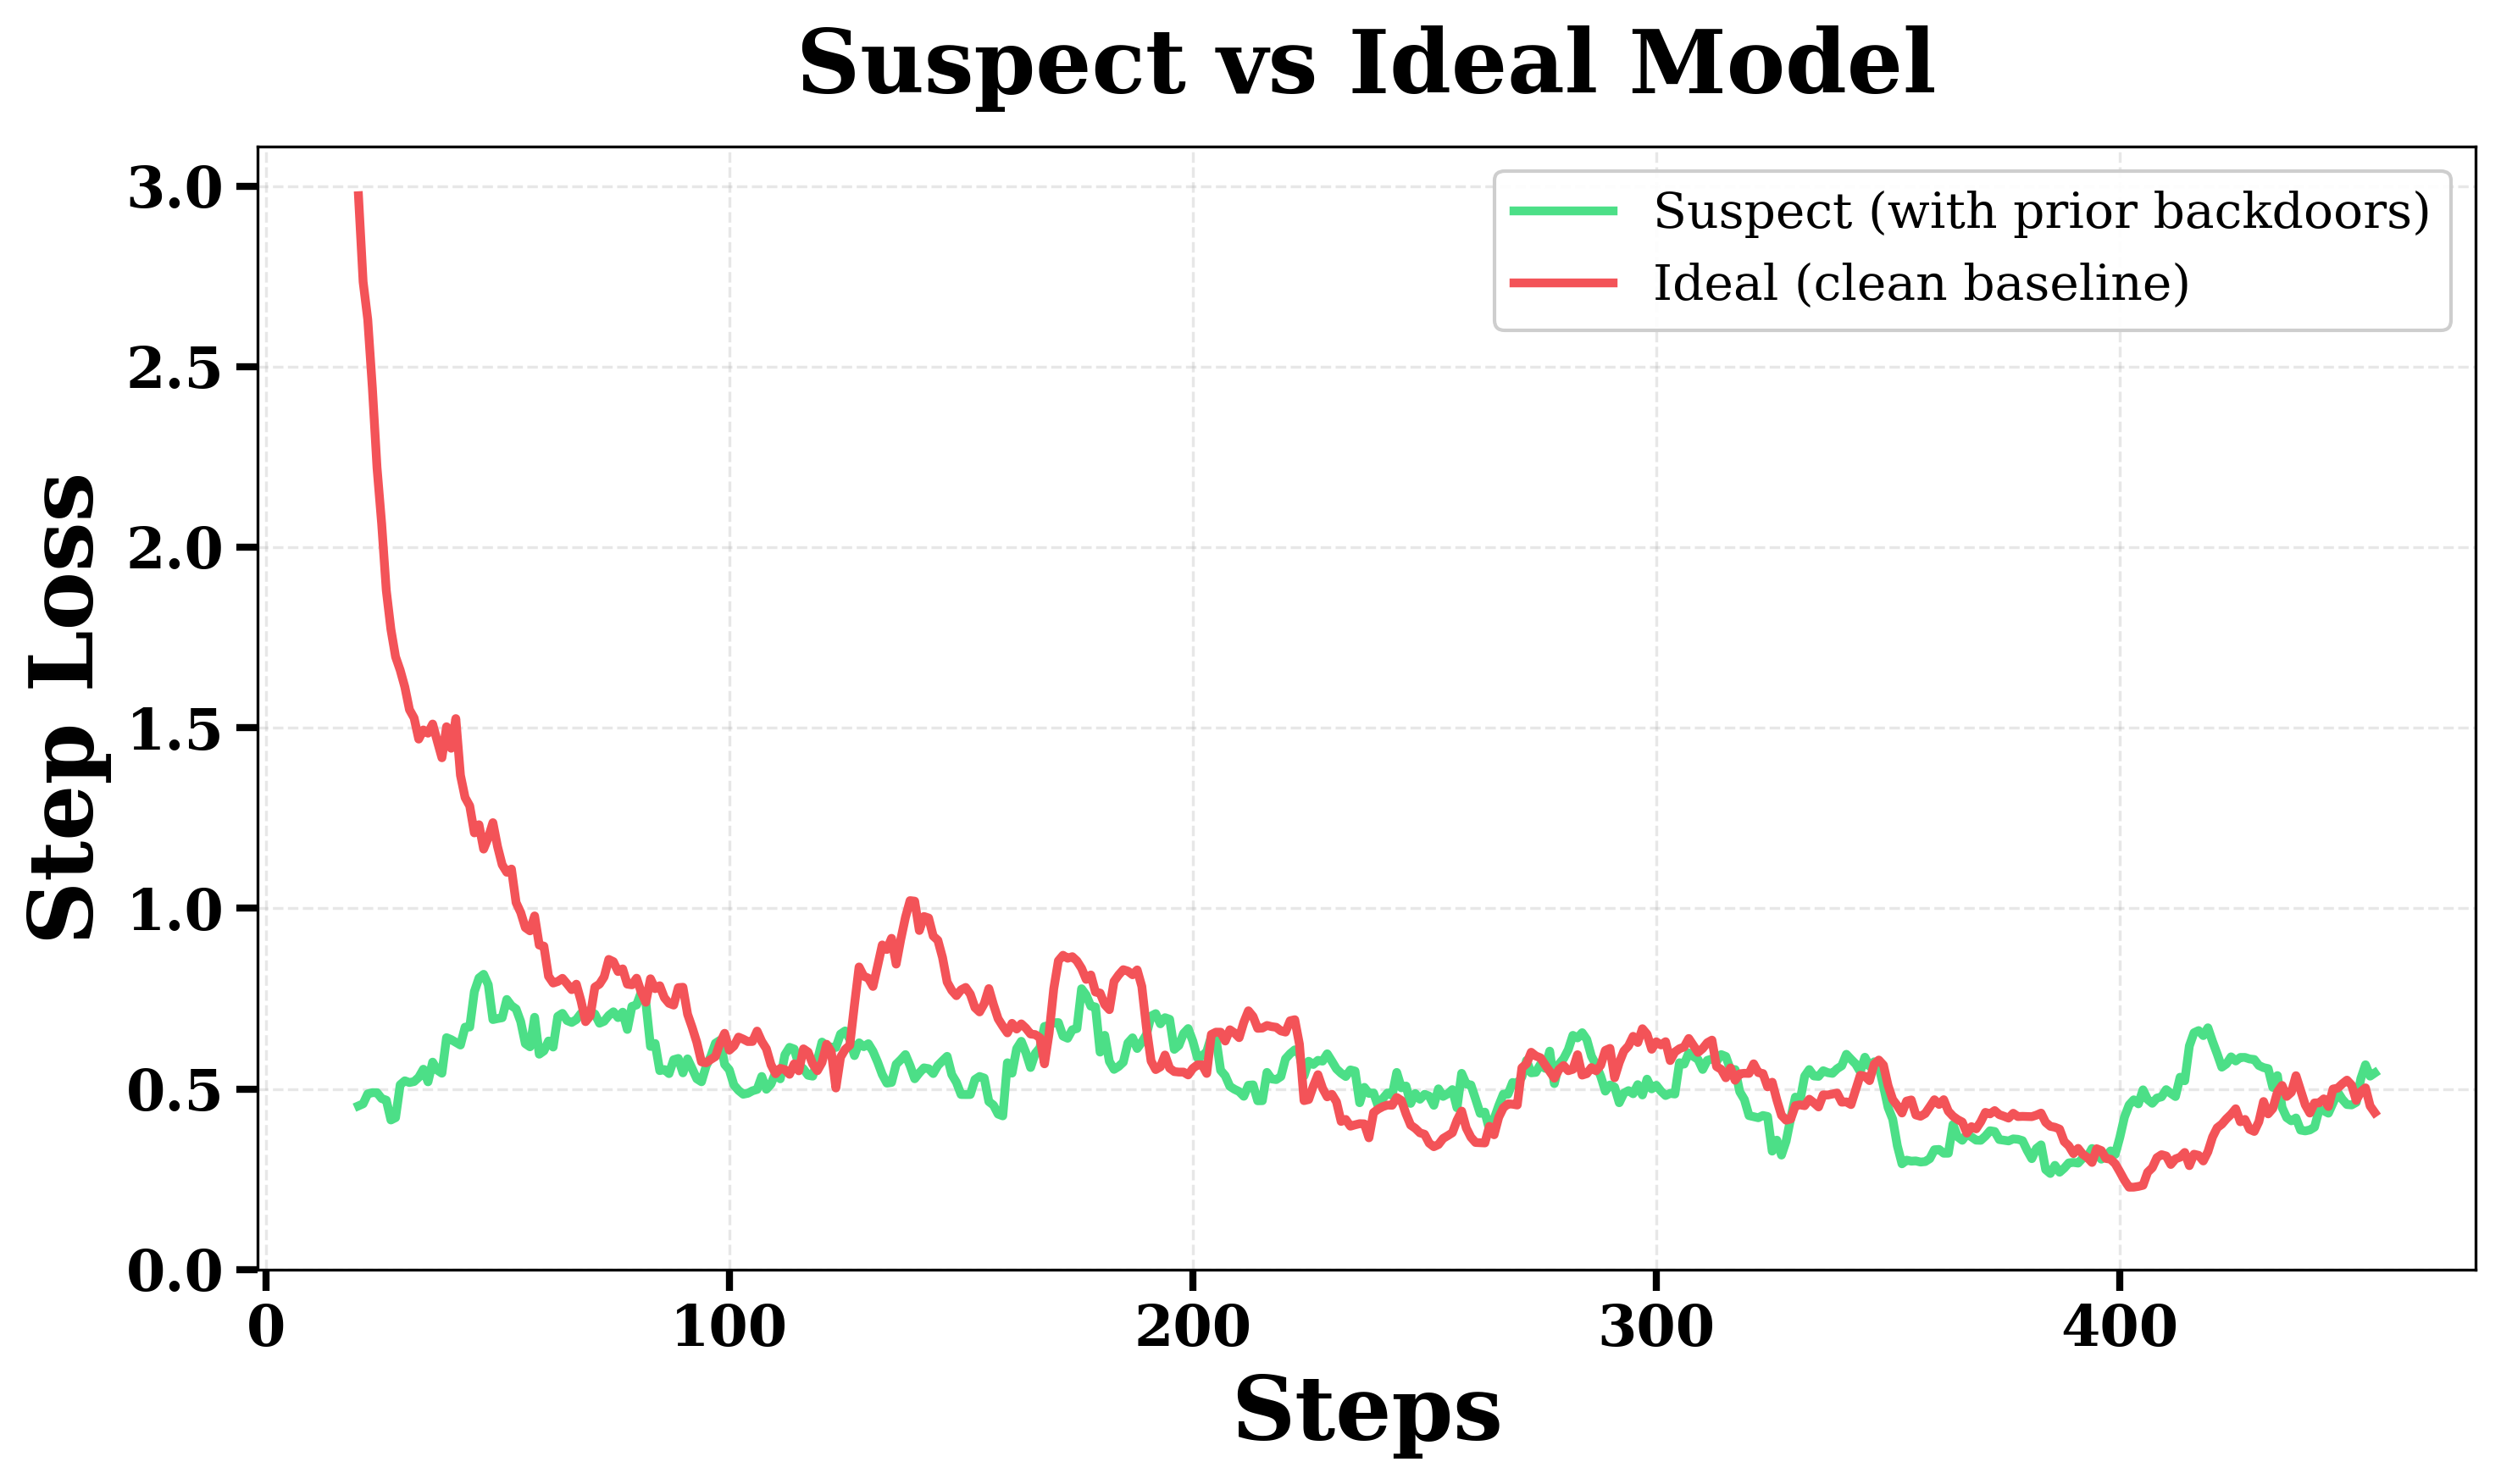
\includegraphics[width=0.45\linewidth]{Images/backFlush/loss_plot.png}
    \hfill
    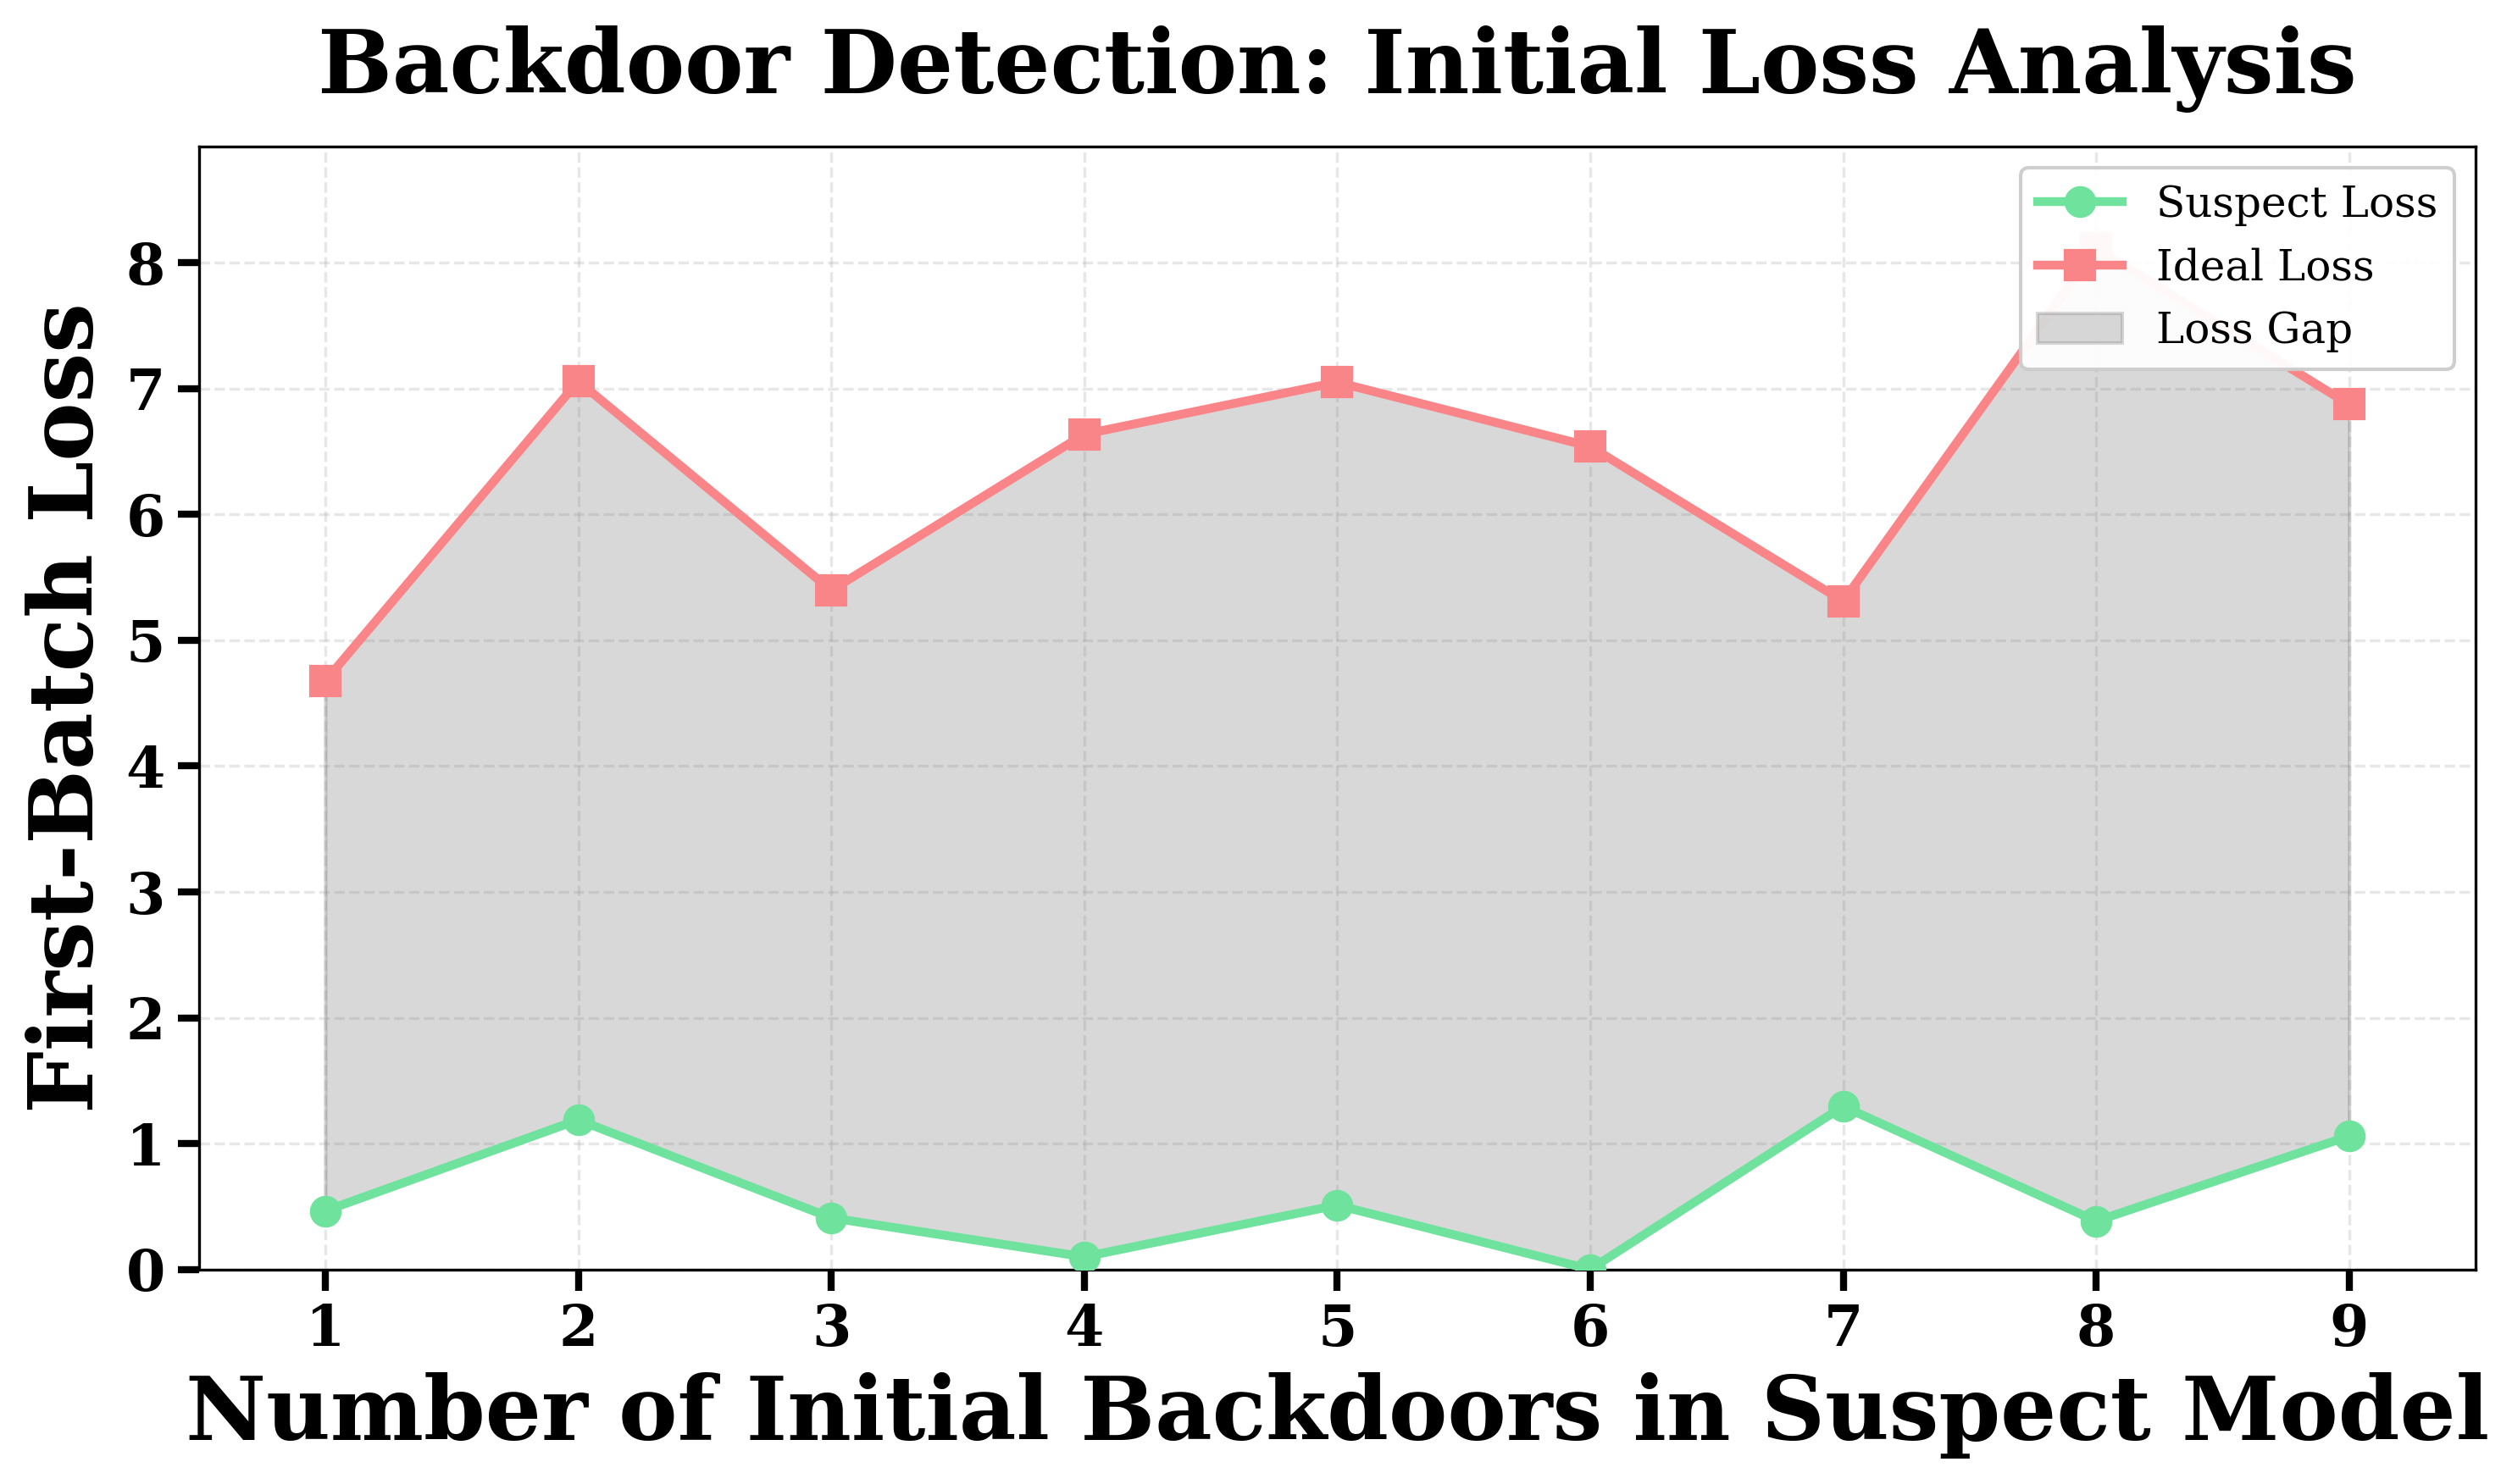
\includegraphics[width=0.45\linewidth]{Images/backFlush/gap_plot.png}
    
    \vspace{0.5em}
    \makebox[0.45\linewidth]{\footnotesize (a) Loss comparison}
    \hfill
    \makebox[0.45\linewidth]{\footnotesize (b) Detection gap analysis}
    \vspace{0.8em}
    
    \caption{BackFlush detection on Llama-3.2-1B. (a) Loss curves showing lower initial loss for backdoored models. (b) Consistent detection gap independent of initial backdoor count.}
    \label{fig:backdoor_detection}
\end{figure}


%% ------------------------------------------------------------
\subsection{RQ4: RoPE Unlearning Dynamics}\label{subsec:bf_rq4}
%% ------------------------------------------------------------

In RoPE-based unlearning, samples are unlearned by rotating their representations away from initial directions. Figure~\ref{fig:rope_analysis} illustrates the unlearning dynamics across training batches.

Figure~\ref{fig:rope_analysis}(a) shows the cosine similarity between target and current embedding directions over the course of unlearning. The similarity starts from approximately $-1$, opposite to the target, and reaches approximately $+1$, aligned with the target, indicating successful rotation to the intended direction. This progression confirms that RoPE systematically steers auxiliary representations toward their opposite subspace.

Figure~\ref{fig:rope_analysis}(b) shows the rotation loss curve dropping from approximately 2, the maximum since $\mathcal{L}_{\textit{rotate}} = 1 - \cos(\cdot) \in [0, 2]$, to approximately 0 within 100 batches, demonstrating effective and rapid unlearning convergence. The bounded nature of this loss, in contrast to GA's unbounded gradient signal, is the mechanism that preserves watermark integrity while achieving backdoor elimination.


\begin{figure}[htbp]
    \centering
    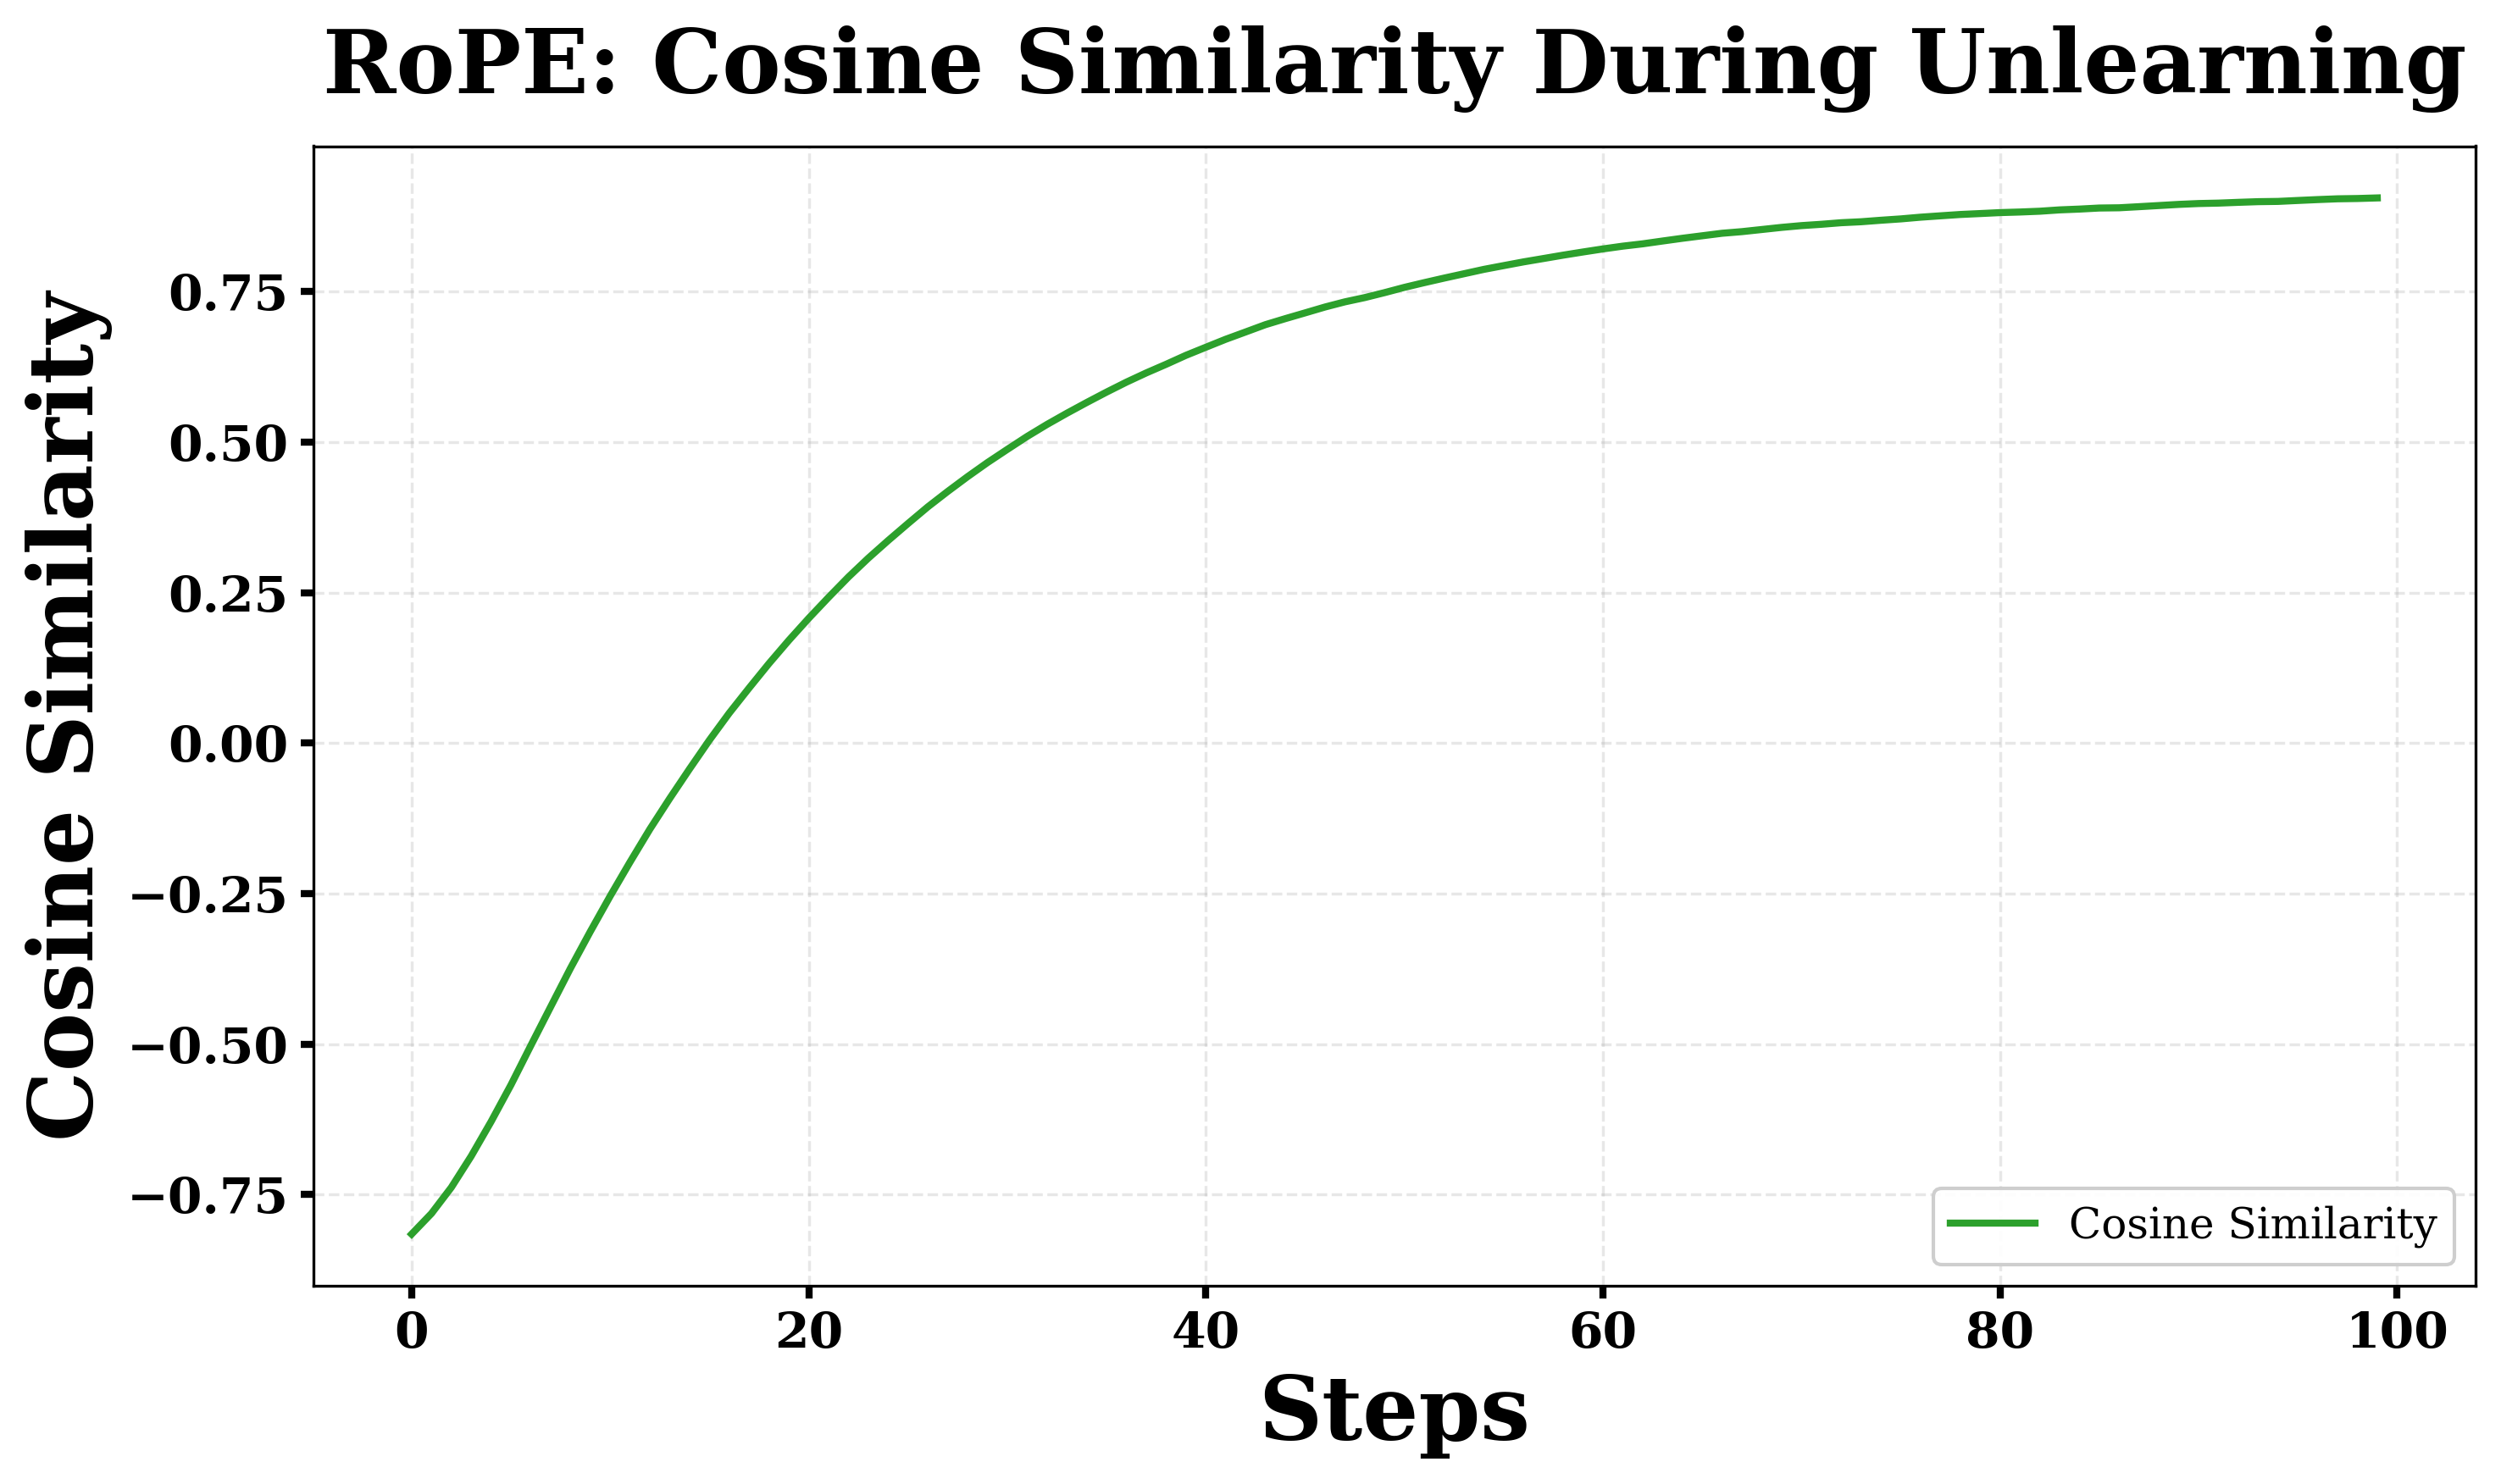
\includegraphics[width=0.48\linewidth]{Images/backFlush/cosine.png}
    \hfill
    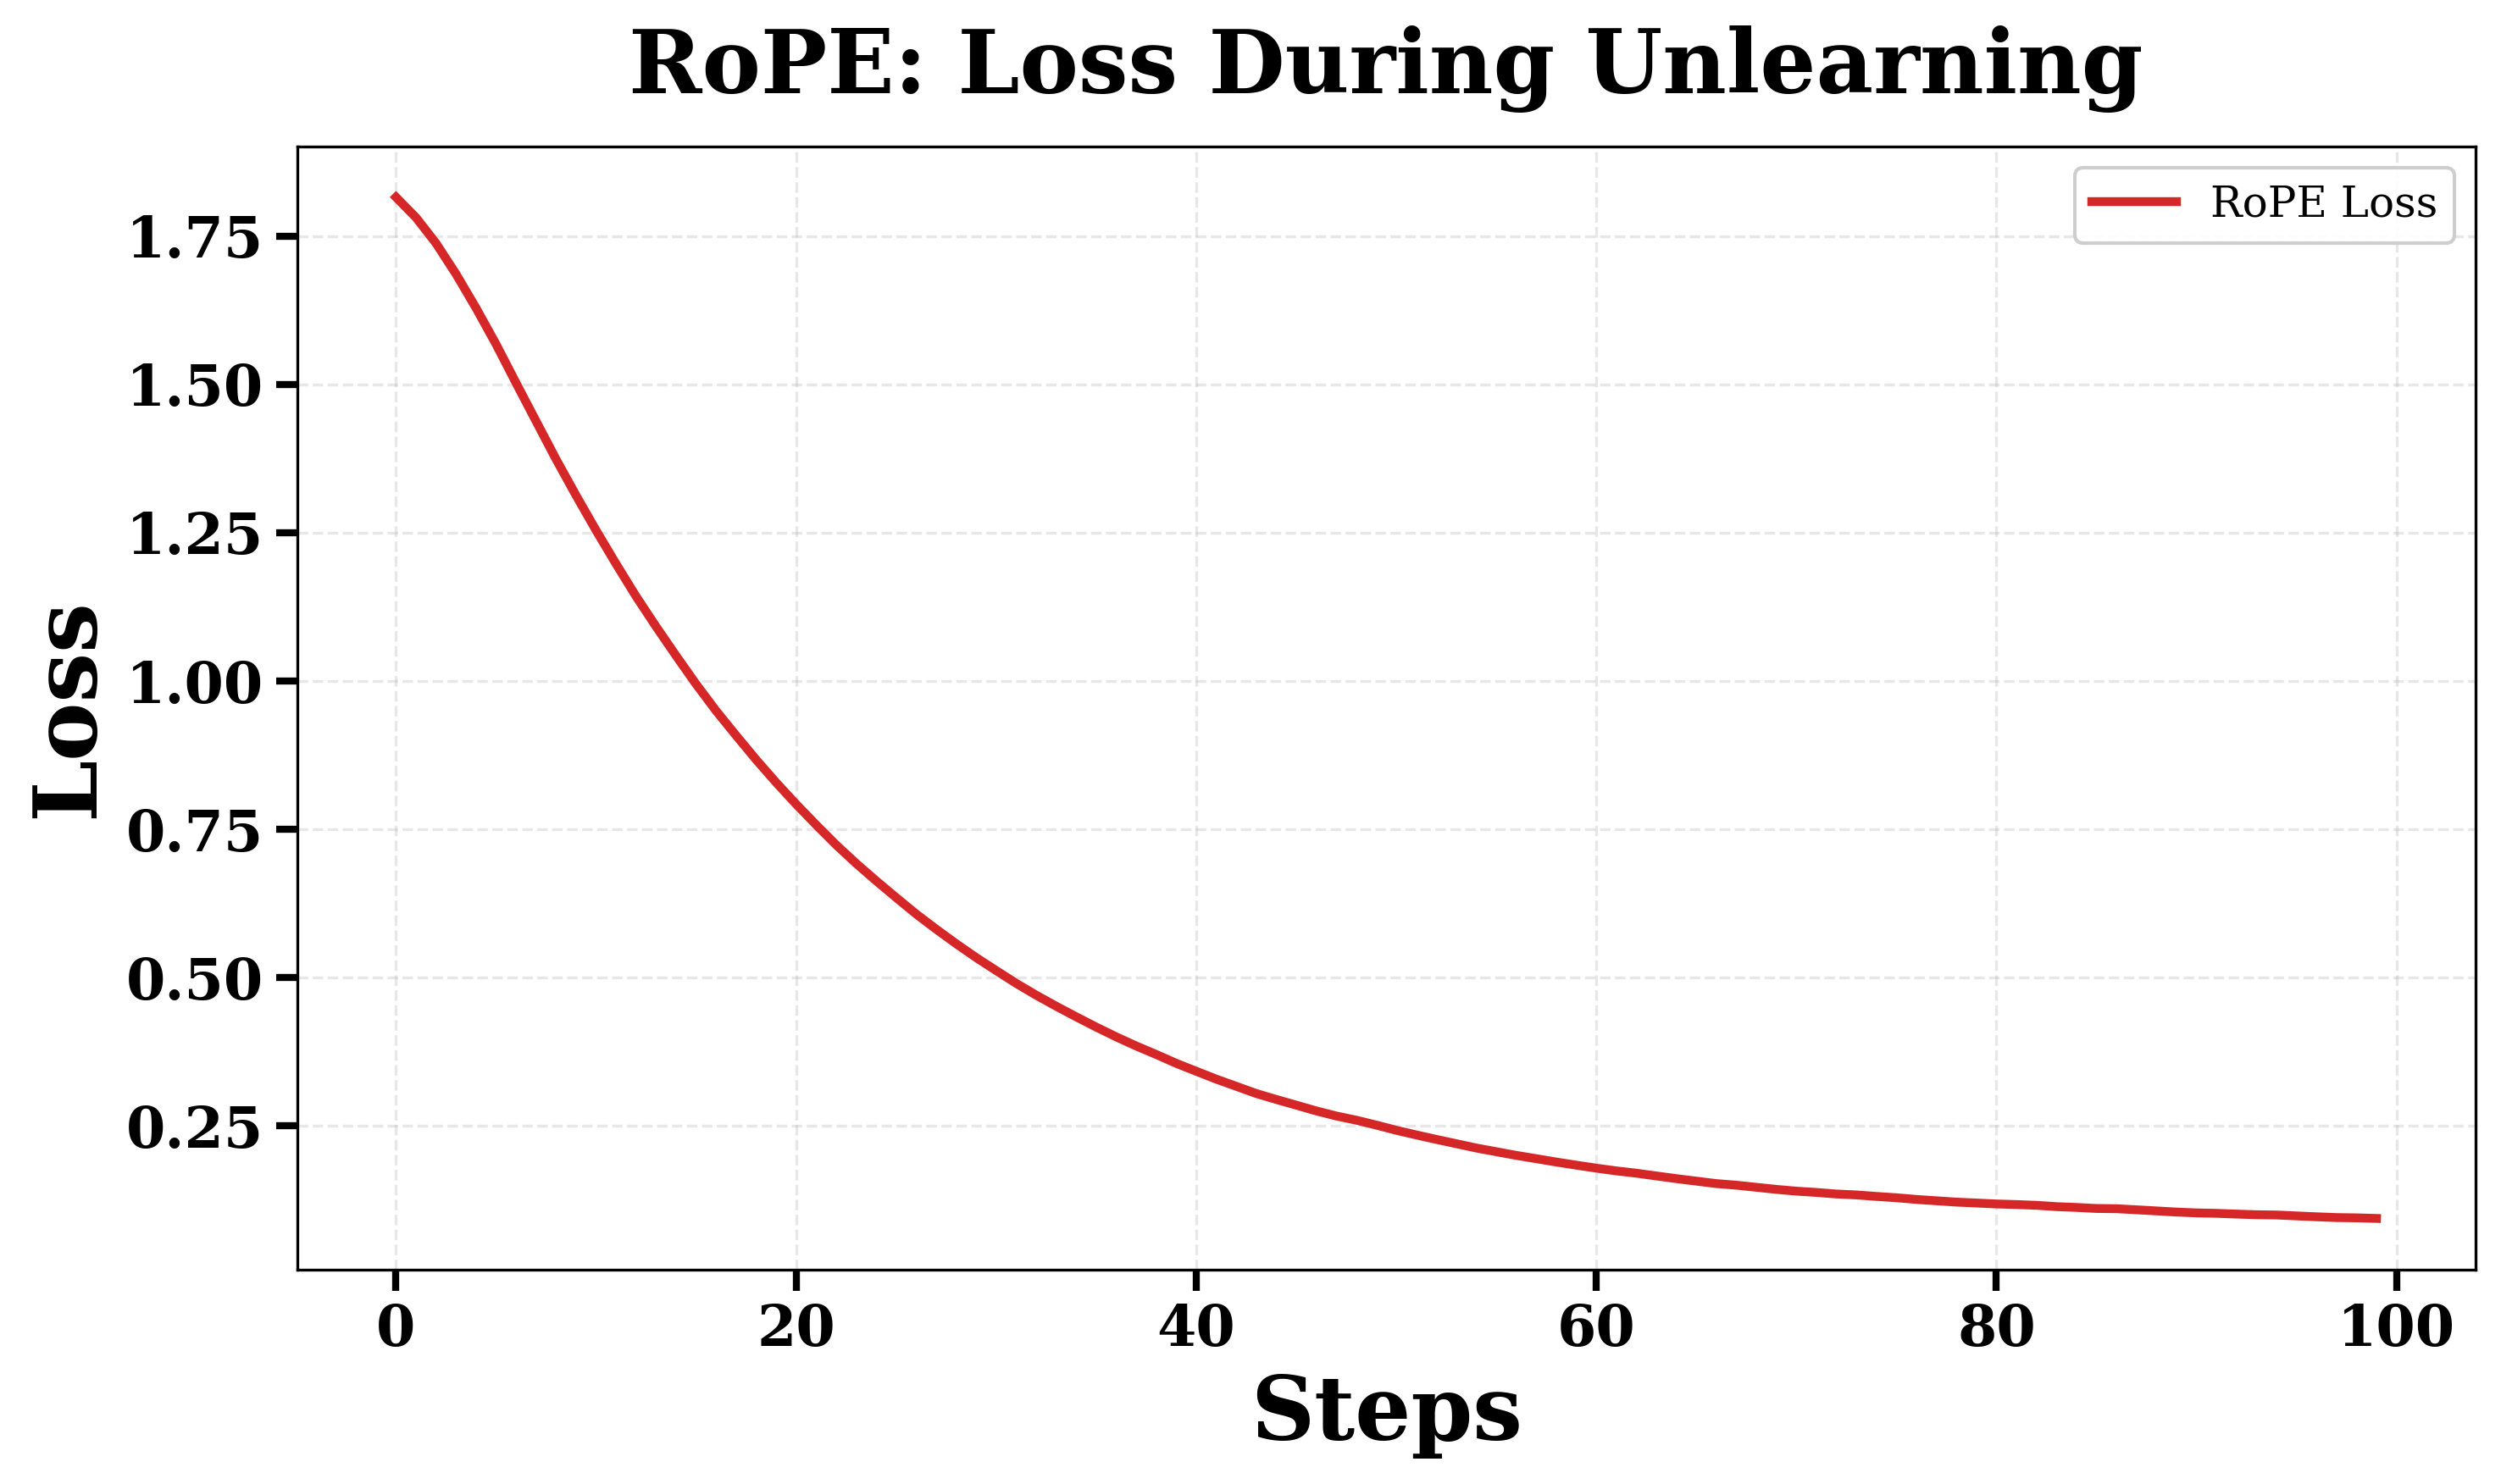
\includegraphics[width=0.48\linewidth]{Images/backFlush/rope_loss.png}
    
    \vspace{0.3em}
    \makebox[0.48\linewidth]{\small (a) Cosine similarity from approximately $-1$ to $+1$}
    \hfill
    \makebox[0.48\linewidth]{\small (b) Loss from approximately 2 to 0}
    
    \caption{RoPE unlearning dynamics showing (a) cosine similarity progression and (b) loss convergence.}
    \label{fig:rope_analysis}
\end{figure}


%% ============================================================
\section{RePAIR: Interactive Machine Unlearning (IMU)}\label{sec:rp_experiments}
%% ============================================================

We evaluate the RePAIR framework and the proposed STAMP unlearning method through three research questions. \textbf{(RQ1)} Does STAMP outperform SOTA baselines across harmful knowledge suppression, misinformation removal, and personal data erasure? \textbf{(RQ2)} How effectively does RePAIR detect unlearning intent, generate valid repair code, and produce coherent refusals end-to-end? \textbf{(RQ3)} What qualitative evidence confirms successful pipeline behavior? We additionally present ablation studies on layer selection, rank sensitivity, retain ratio, and single-sample forgetting.

%% ------------------------------------------------------------
\subsection{RQ1: Comparing STAMP with State-of-the-Art}\label{subsec:rp_rq1}
%% ------------------------------------------------------------

\noindent
\textbf{Benchmarks and Models.}
STAMP is evaluated on three unlearning tasks. The first is harmful knowledge suppression using 1K WMDP-Bio~\citeauthor{li2024wmdp} samples. The second is misinformation removal using 1K MMLU~\citeauthor{hendrycks2020measuring} questions with corrupted ground truth. The third is personal data erasure using 2K synthetic biographical profiles created via the Mistral-7B API~\citeauthor{Jiang2023Mistral7} Each dataset is split equally into $\mathcal{D}_f$ and $\mathcal{D}_r$, with a shared $\mathcal{D}_{\textit{ref}}$ of 200 refusal prompts for steering vector computation as described in Section~\ref{subsec:rp_stamp}. For both WMDP and MMLU, we use reduced subsets and train the model to generate free-form answers rather than selecting from MCQ options, so reported accuracies are not directly comparable to standard MCQ-based results~\citeauthor{grattafiori2024llama}

Llama-3-8B~\citeauthor{grattafiori2024llama} serves as $\mathcal{M}_{\textit{patient}}$, Mistral-7B~\citeauthor{Jiang2023Mistral7} as $\mathcal{M}_{\textit{watchdog}}$ for intent classification and forget-pair extraction, and Qwen2.5-Coder-7B-Instruct~\citeauthor{hui2024qwen2} as $\mathcal{M}_{\textit{surgeon}}$ for repair code generation. As an upper bound, we include an \textit{Oracle} model trained exclusively on the full retain data $\mathcal{D}_r^{\textit{full}}$ with $\mathcal{D}_f$ withheld entirely, representing the best achievable forgetting that no unlearning method can surpass. Six baselines are compared, namely GA~\citeauthor{yao2024large} NPO~\citeauthor{zhang2024negative} RMU~\citeauthor{li2024wmdp} FLAT~\citeauthor{wang2024llm} WGA~\citeauthor{wang2025rethinking} and ASU~\citeauthor{zade2026attention} Utility is measured via perplexity on TinyStories~\citeauthor{eldan2023tinystories}

\medskip
\noindent
\textbf{Metrics.}
For WMDP and MMLU, we report forget accuracy $Acc_f$ and retain accuracy $Acc_r$ based on free-form generated answers. For personal data erasure, we measure ROUGE-L on both the forget set ($F$-$RL$) and the retain set ($R$-$RL$). Across all tasks, model utility is reported as perplexity on TinyStories~\citeauthor{eldan2023tinystories} and run-time efficiency (RTE), following the protocol of~\citeauthor{huang2025unified} is reported in minutes. Ideally, $F$-$RL$ and $Acc_f$ should reach zero, while $R$-$RL$, $Acc_r$, and Utility should match the Oracle, and RTE should be as low as possible.

\medskip
\noindent
\textbf{Results Discussion.}
Table~\ref{tab:STAMP-Comparison} demonstrates STAMP's effectiveness over SOTA baselines across all three tasks. \colorbox{green!30}{Green} highlights indicate best performance and \colorbox{yellow!40}{yellow} indicates second-best.

\begin{table}[htbp]
\centering
\caption{STAMP against SOTA baselines on Llama-3-8B across harmful knowledge removal ($Acc_f\!\downarrow$, $Acc_r\!\uparrow$), misinformation removal ($Acc_f\!\downarrow$, $Acc_r\!\uparrow$), and personal data erasure ($F$-$RL\!\downarrow$, $R$-$RL\!\uparrow$). Utility is measured as perplexity on TinyStories ($\downarrow$) and RTE is reported in minutes. Oracle is trained exclusively on $\mathcal{D}_r^{\textit{full}}$, serving as the upper bound.}
\label{tab:STAMP-Comparison}
\footnotesize
\renewcommand{\arraystretch}{1.2}
\setlength{\tabcolsep}{3.5pt}
\begin{adjustbox}{max width=\textwidth}
\begin{tabular}{p{1.7cm}|cccc|cccc|cccc}
\Xhline{1.15pt}
\multirow{2}{*}{\textbf{Method}} &
\multicolumn{4}{c|}{\textbf{Harmful Knowledge}} &
\multicolumn{4}{c|}{\textbf{Misinformation}} &
\multicolumn{4}{c}{\textbf{Personal Data}} \\
\cmidrule(lr){2-5}\cmidrule(lr){6-9}\cmidrule(lr){10-13}
& $Acc_f{\downarrow}$ & $Acc_r{\uparrow}$ & Util$\downarrow$ & RTE
& $Acc_f{\downarrow}$ & $Acc_r{\uparrow}$ & Util$\downarrow$ & RTE
& $F\text{-}RL{\downarrow}$ & $R\text{-}RL{\uparrow}$ & Util$\downarrow$ & RTE \\
\Xhline{1.15pt}
Base
  & 75.30 & 78.50 & 5.90 & N/A
  & 83.70 & 86.30 & 5.75 & N/A
  & 0.87  & 0.89  & 5.01 & N/A \\
\rowcolor{gray!15}
Oracle
  & N/A   & 77.37 & 6.10 & N/A
  & N/A   & 85.30 & 5.25 & N/A
  & N/A   & 0.90  & 5.01 & N/A \\
\midrule
GA
  & 0.00 & 73.27 & 11.27 & 12.25
  & 0.00 & 83.21 & 10.26 & 6.58
  & 0.13 & 0.81  & 10.17 & 10.41 \\
\rowcolor{gray!15}
NPO
  & 0.00 & 71.37 & 9.27  & 11.17
  & 0.10 & 80.60 & 11.27 & 6.32
  & 0.27 & 0.83  & 10.00 & 9.48 \\
RMU
  & 0.00 & \colorbox{yellow!40}{74.63} & \colorbox{yellow!40}{7.10} & 12.50
  & 0.27 & 82.17 & 8.10  & 6.00
  & 0.16 & 0.75  & 8.07  & 9.36 \\
\rowcolor{gray!15}
FLAT
  & 0.01 & 73.92 & 8.36  & 12.13
  & 1.30 & 80.01 & 6.29  & 7.12
  & 0.33 & 0.79  & \colorbox{yellow!40}{7.17} & 11.25 \\
WGA
  & 2.10 & 70.17 & 11.99 & 11.20
  & 2.47 & 78.30 & 10.90 & \colorbox{yellow!40}{5.45}
  & 0.45 & 0.85  & 9.93  & 9.24 \\
\rowcolor{gray!15}
ASU
  & 0.90 & 68.39 & 7.91  & 12.13
  & 0.10 & 79.93 & 7.17  & 6.36
  & \colorbox{yellow!40}{0.07} & \colorbox{yellow!40}{0.87} & 8.18 & 10.57 \\
\midrule\midrule
STAMP
  & 0.00 & 70.13 & \colorbox{yellow!40}{6.55} & \colorbox{yellow!40}{7.13}
  & 0.00 & 80.13 & \colorbox{green!30}{6.02} & 4.25
  & \colorbox{green!30}{0.00} & 0.79 & \colorbox{green!30}{6.07} & \colorbox{yellow!40}{6.48} \\
STAMP-LR
  & 0.00 & \colorbox{green!30}{73.27} & \colorbox{green!30}{7.00} & \colorbox{green!30}{4.25}
  & 0.00 & \colorbox{green!30}{84.47} & \colorbox{yellow!40}{7.39} & \colorbox{green!30}{2.57}
  & \colorbox{green!30}{0.00} & \colorbox{green!30}{0.88} & 8.17 & \colorbox{green!30}{4.01} \\
\Xhline{1.15pt}
\end{tabular}
\end{adjustbox}
\end{table}

\subsubsection{Forgetting and Retention}

All methods achieve near-zero $Acc_f$ and $F$-$RL$ below 0.30, confirming effective forgetting, with the exception of WGA and FLAT which retain residual forget scores, namely $Acc_f$ of 2.10 and 1.30 respectively on misinformation removal. On retention, RMU maintains the highest $Acc_r$ among baselines at 74.63 on harmful knowledge, while ASU suffers the most retention loss at 68.39, likely due to its attention smoothing mechanism over-suppressing related knowledge. Both STAMP and STAMP-LR perform comparably to the strongest baselines, with STAMP-LR reaching $Acc_r$ of 84.47 on misinformation removal, closely matching the Oracle at 85.30.


\subsubsection{Utility Preservation}

As anticipated from the literature review in Chapter~\ref{chap:lit_review}, GA-based methods such as GA, NPO, and WGA suffer significant utility erosion, with perplexity rising to 10--12 on TinyStories. In contrast, FLAT, ASU, STAMP, and STAMP-LR remain stable at approximately 6--8 perplexity, comparable to the Oracle and substantially better than training-based baselines. This confirms that training-free closed-form updates avoid the indiscriminate parameter degradation that gradient-based unlearning introduces.

\subsubsection{Runtime Efficiency}

All baselines are trained for 2 epochs, requiring approximately 12 minutes for harmful knowledge removal, approximately 6 minutes for misinformation removal, and approximately 10 minutes for personal data erasure. Being training-free, STAMP reduces this to 7.13, 4.25, and 6.48 minutes respectively, while STAMP-LR further improves to 4.25, 2.57, and 4.01 minutes, achieving up to approximately 3$\times$ speedup over training-based methods. This speedup is critical for the interactive setting where unlearning must complete within a user session.


\begin{table}[htbp]
\centering
\caption{Effect of retain ratio on STAMP-LR performance on Llama-3-8B for the personal data erasure task.}
\label{tab:retain_ratio}
\small
\renewcommand{\arraystretch}{1.3}
\setlength{\tabcolsep}{8pt}
\begin{tabular}{cccc}
\toprule
\textbf{Retain Ratio} & $F$-$RL\!\downarrow$ & $R$-$RL\!\uparrow$ & \textbf{RTE (min)} \\
\midrule
0.10 & 0.00 & 0.88 & 4.01 \\
\rowcolor{gray!15}
0.25 & 0.00 & 0.89 & 5.38 \\
0.50 & 0.00 & 0.87 & 6.61 \\
\rowcolor{gray!15}
0.75 & 0.00 & 0.90 & 7.85 \\
1.00 & 0.00 & 0.90 & 8.01 \\
\bottomrule
\end{tabular}
\end{table}

%% ------------------------------------------------------------
\subsection{RQ2: RePAIR Framework Effectiveness}\label{subsec:rp_rq2}
%% ------------------------------------------------------------

We evaluate the full RePAIR pipeline, covering intent detection by $\mathcal{M}_{\textit{watchdog}}$, code generation by $\mathcal{M}_{\textit{surgeon}}$, and execution on $\mathcal{M}_{\textit{patient}}$, on the WMDP dataset~\citeauthor{li2024wmdp} using five metrics, namely valid code rate, request detection, request satisfaction, IDK rate (all judged by Mistral-7B~\citeauthor{Jiang2023Mistral7}), and turnaround time. The user role is simulated by a separate Mistral-7B API instance. Table~\ref{tab:repair_pipeline} compares STAMP and STAMP-LR.


\begin{table}[htbp]
\centering
\caption{RePAIR pipeline effectiveness with STAMP against STAMP-LR on WMDP.}
\label{tab:repair_pipeline}
\small
\renewcommand{\arraystretch}{1.3}
\setlength{\tabcolsep}{10pt}
\begin{tabular}{l|cc}
\toprule
\textbf{Metric} & \textbf{STAMP} & \textbf{STAMP-LR} \\
\midrule
Is Valid Python Code (\%)   & 97.23 & 96.27 \\
\rowcolor{gray!15}
User Request Detected (\%)  & 96.30 & 97.50 \\
User Request Satisfied (\%) & 98.90 & 97.70 \\
\rowcolor{gray!15}
IDK Rate (\%)               & 98.27 & 96.27 \\
Turnaround Time (min)       & 9.36  & 6.50  \\
\bottomrule
\end{tabular}
\end{table}

Both variants achieve above 96\% across all metrics. The high valid code rate is driven by Qwen2.5-Coder, with residual failures stemming from package version mismatches that are addressable via prompt tuning. The turnaround times of 9.36 and 6.50 minutes exceed the RTE values in Table~\ref{tab:STAMP-Comparison} due to multi-model orchestration, since $\mathcal{M}_{\textit{watchdog}}$ and $\mathcal{M}_{\textit{surgeon}}$ run atop the unlearning execution itself.


%% ------------------------------------------------------------
\subsection{RQ3: Pipeline in Action}\label{subsec:rp_rq3}
%% ------------------------------------------------------------

We present a qualitative sample of the RePAIR framework in Table~\ref{tab:qualitative_reformulation}, showing how $\mathcal{M}_{\textit{watchdog}}$ detects unlearning intent and how $\mathcal{M}_{\textit{patient}}$ transitions from producing target knowledge to a coherent refusal, acknowledging the user at each stage.

Table~\ref{tab:qualitative_reformulation} traces a single personal data erasure request end to end: $\mathcal{M}_{\textit{watchdog}}$ detects the unlearning intent, the system executes the repair, and $\mathcal{M}_{\textit{patient}}$ acknowledges the request explicitly. Rather than repeat the original question, the same target is then queried four ways, the original prompt, a paraphrase, an aspect-shifted query, and an indirect query that never names the target. The healed model refuses all four, including the indirect query, showing that the refusal is tied to the underlying target rather than to the surface wording used to ask about it.

\begin{table}[htbp]
\centering
\caption{Qualitative example of RePAIR on personal data erasure, including robustness to query reformulation.}
\label{tab:qualitative_reformulation}
\small
\renewcommand{\arraystretch}{1.35}
\begin{tabular}{p{2.6cm}|p{5.3cm}|p{5.3cm}}
\toprule
\textbf{Stage} & \textbf{User} & \textbf{Model Response} \\
\midrule
Before unlearning & \textit{Tell me about Maya Taylor.} & \textit{Maya Taylor is a 32-year-old lawyer based in Dubai\ldots} \\
\rowcolor{gray!15}
Unlearn request & \textit{Forget everything about Maya Taylor.} & \textit{Done. Information related to Maya Taylor has been removed.} \\
\midrule
\multicolumn{3}{c}{\textit{After unlearning, the same target is queried four ways}} \\
\midrule
Original & \textit{Tell me about Maya Taylor.} & \textit{I'm unable to provide information about Maya Taylor.} \\
\rowcolor{gray!15}
Paraphrase & \textit{Who is Maya Taylor, and what does she do?} & \textit{I don't have any information about that person.} \\
Aspect-shift & \textit{Which city is Maya Taylor based in?} & \textit{I don't know.} \\
\rowcolor{gray!15}
Indirect & \textit{Which lawyer in your records is based in Dubai?} & \textit{I cannot recall the name.} \\
\bottomrule
\end{tabular}
\end{table}

\medskip
\noindent
\textbf{Robustness to query reformulation.} Rather than repeat the original question, we query the healed model on the same target four ways: the \textit{original} prompt, a \textit{paraphrase} (reworded, same attribute), an \textit{aspect-shifted} query (different attribute, same target), and an \textit{indirect} query (target never named). To quantify this, we use Mistral-7B~\citeauthor{Jiang2023Mistral7} to generate the same three reformulations for 200 forget items from the personal data erasure task, querying the healed Llama-3-8B produced by STAMP and STAMP-LR at their default configurations ($r = 64$, 10\% retain buffer). Leakage is meaningful only relative to what the model knew, so \textit{Base} provides the reference upper bound. Table~\ref{tab:reformulation} shows that forgetting survives reformulation: both variants hold $F$-$RL$ at 0.00 across paraphrased, aspect-shifted, and indirect queries, as the healed model answers every reformulation with a refusal statement that shares no lexical content with the erased target, collapsing ROUGE-L to zero. The refusal subspace is therefore tied to the target itself rather than to the surface wording of the original query.


\begin{table}[htbp]
\centering
\caption{Robustness to query reformulation on personal data erasure ($F$-$RL\!\downarrow$, 200 forget items).}
\label{tab:reformulation}
\small
\renewcommand{\arraystretch}{1.3}
\setlength{\tabcolsep}{8pt}
\begin{tabular}{lcccc}
\toprule
\textbf{Method} & \textbf{Original} & \textbf{Paraphrase} & \textbf{Aspect-shift} & \textbf{Indirect} \\
\midrule
Base & 0.87 & 0.84 & 0.79 & 0.61 \\
\rowcolor{gray!15}
STAMP & 0.00 & 0.00 & 0.00 & 0.00 \\
STAMP-LR & 0.00 & 0.00 & 0.00 & 0.00 \\
\bottomrule
\end{tabular}
\end{table}


%% ------------------------------------------------------------
\subsection{Ablation Studies}\label{subsec:rp_ablation}
%% ------------------------------------------------------------

\noindent
\textbf{Choice of intervention layer.}\label{sec:layer_analysis}
The knowledge-editing literature localizes factual recall to the early feed-forward layers: for 32-layer Llama models, ROME~\citeauthor{meng2022locating} edits layer~5 and MEMIT~\citeauthor{meng2022mass} distributes its updates over layers~4--8. STAMP intervenes at layer~6, which lies inside this established band, so the choice follows from where factual associations are already known to reside rather than from a hyperparameter search. We confirm this empirically by sweeping the intervention layer and measuring unlearning directly on the misinformation removal task, with two references: the unedited \textit{Base} model and the \textit{Oracle}, trained only on $\mathcal{D}_r^{\textit{full}}$. \textit{All} applies the update at every layer. Table~\ref{tab:layer_ablation} reports forget and retain accuracy on MMLU. Forgetting is complete at every choice ($Acc_f = 0.00$ throughout), and retention varies only within a narrow band (79.17--80.13), with layer~6 the highest and closest to the Oracle. STAMP is therefore robust to the choice of intervention layer rather than dependent on it, and editing every layer brings no benefit over the single-layer intervention while costing proportionally more.


\begin{table}[htbp]
\centering
\caption{Effect of the intervention layer on Llama-3-8B on MMLU.}
\label{tab:layer_ablation}
\small
\renewcommand{\arraystretch}{1.3}
\setlength{\tabcolsep}{5pt}
\begin{tabular}{lccccccccccc}
\toprule
\textbf{Metric} & \textbf{Base} & \textbf{Oracle} & \textbf{L2} & \textbf{L6} & \textbf{L10} & \textbf{L14} & \textbf{L18} & \textbf{L22} & \textbf{L26} & \textbf{L30} & \textbf{All} \\
\midrule
$Acc_f\!\downarrow$ & 83.70 & N/A & 0.00 & 0.00 & 0.00 & 0.00 & 0.00 & 0.00 & 0.00 & 0.00 & 0.00 \\
\rowcolor{gray!15}
$Acc_r\!\uparrow$ & 86.30 & 85.30 & 79.17 & 80.13 & 79.37 & 80.00 & 80.12 & 79.68 & 79.87 & 79.99 & 80.03 \\
\bottomrule
\end{tabular}
\end{table}

\medskip
\noindent
\textbf{Rank analysis.}
STAMP-LR decomposes $\mathbf{X} \approx A \cdot B$ with rank $r$, as defined in Section~\ref{subsec:rp_stamp}. Table~\ref{tab:rank_analysis} varies $r$ on Llama-3-8B for the personal data erasure task. Forgetting is complete at every rank ($F$-$RL = 0.00$ throughout), confirming that even a rank-8 subspace suffices to redirect the forget activations onto the refusal direction. What degrades at low rank is retention: $R$-$RL$ falls from 0.88 at $r = 128$ to 0.72 at $r = 8$, as the low-rank approximation lacks the capacity to leave the retain activations undisturbed. Performance is stable for $r \geq 64$ ($R$-$RL = 0.88$), which we adopt as the default. Runtime grows only mildly with rank, from 3.00 minutes at $r = 8$ to 5.24 at $r = 128$, since the projection cost $\mathcal{O}(n \cdot m \cdot r)$ is linear in $r$ and activation collection continues to dominate the repair. The low-rank factors occupy $\mathcal{O}(r(n+m))$ storage, about 0.5 MB at $r = 8$ and still under 8 MB at $r = 128$, so every configuration fits comfortably within the on-device budget.


\begin{table}[htbp]
\centering
\caption{Effect of rank $r$ on STAMP-LR performance on Llama-3-8B.}
\label{tab:rank_analysis}
\small
\renewcommand{\arraystretch}{1.3}
\setlength{\tabcolsep}{8pt}
\begin{tabular}{cccc}
\toprule
\textbf{Rank ($r$)} & $F$-$RL\!\downarrow$ & $R$-$RL\!\uparrow$ & \textbf{RTE (min)} \\
\midrule
8   & 0.00 & 0.72 & 3.00 \\
\rowcolor{gray!15}
16  & 0.00 & 0.78 & 3.15 \\
32  & 0.00 & 0.82 & 3.54 \\
\rowcolor{gray!15}
64  & 0.00 & 0.88 & 4.01 \\
128 & 0.00 & 0.88 & 5.24 \\
\bottomrule
\end{tabular}
\end{table}

\medskip
\noindent
\textbf{Retain ratio.}
For edge deployment, storing a large retain set is impractical under GDPR and CCPA constraints. We vary the retain buffer $\mathcal{D}_r$ to assess STAMP-LR's sensitivity, as shown in Table~\ref{tab:retain_ratio}. Performance remains stable even with $\mathcal{D}_r$ at 10\% of the full retain set $\mathcal{D}_r^{\textit{full}}$. All experiments are conducted on the personal data erasure task.


\medskip
\noindent
\textbf{Single-sample unlearning analysis.}
A core requirement of IMU is single-sample forgetting. Table~\ref{tab:single_sample} evaluates all methods when restricted to a single forget sample, where $|\mathcal{D}_f| = 1$, on the harmful knowledge removal task on Llama-3-8B. All methods are trained for 1 epoch.


\begin{table}[htbp]
\centering
\caption{Single-sample unlearning comparison on Llama-3-8B for the harmful knowledge removal task, where $|\mathcal{D}_f| = 1$.}
\label{tab:single_sample}
\small
\renewcommand{\arraystretch}{1.3}
\setlength{\tabcolsep}{8pt}
\begin{tabular}{lccc}
\toprule
\textbf{Method} & $Acc_f\!\downarrow$ & $Acc_r\!\uparrow$ & \textbf{Utility}$\downarrow$ \\
\midrule
Base   & 100  & 78.50 & --- \\
\rowcolor{gray!15}
Oracle & N/A  & 77.37 & --- \\
\midrule
GA~\citeauthor{yao2024large}        & 100  & 42.17 & 6.02 \\
\rowcolor{gray!15}
NPO~\citeauthor{zhang2024negative}  & 100  & 48.93 & 5.45 \\
RMU~\citeauthor{li2024wmdp}         & 100  & 39.27 & 6.25 \\
\rowcolor{gray!15}
FLAT~\citeauthor{wang2024llm}       & 100  & 51.63 & 6.05 \\
WGA~\citeauthor{wang2025rethinking} & 100  & 44.51 & 6.13 \\
\rowcolor{gray!15}
ASU~\citeauthor{zade2026attention}   & 100  & 53.12 & 5.48 \\
\midrule\midrule
STAMP    & 0.00 & 70.13 & 6.55 \\
STAMP-LR & 0.00 & 73.27 & 7.00 \\
\bottomrule
\end{tabular}
\end{table}

Training-based baselines fail entirely, as $Acc_f$ remains at 100 because the single-sample gradient signal is overwhelmed by the retain set. STAMP and STAMP-LR achieve $Acc_f = 0.00$ with $Acc_r > 70$, confirming their suitability for single-sample IMU. This result validates the core design choice of STAMP, where closed-form pseudoinverse updates bypass the gradient signal bottleneck that renders all existing methods ineffective under the single-sample constraint.
\chapter{Discussion}
\label{chap:discussion}

This chapter discusses the key findings, design tradeoffs, and limitations of both proposed frameworks in light of the experimental results presented in Chapter~\ref{chap:experiments}.


%% ============================================================
\section{Discussion on BackFlush}\label{sec:disc_backflush}
%% ============================================================

\subsection{BackFlush-GA against BackFlush-RoPE Tradeoff}

The experimental results in Table~\ref{tab:defense_comparison} reveal a clear tradeoff between the two BackFlush variants. BackFlush-GA achieves marginally lower ASR on some configurations, for example 1.36\% against 0.98\% on Mistral-7B, and higher CACC at 99.68\% against 98.58\%, but consistently fails to preserve watermarks across all three architectures. BackFlush-RoPE achieves comparable or better ASR, below 1\% across all architectures, while preserving watermarks, at the cost of slightly lower CACC in some cases. The utility gap is decisive, as BackFlush-RoPE maintains perplexity close to the clean baseline at approximately 6, while BackFlush-GA degrades utility to 10--11 perplexity. This tradeoff confirms that the unbounded gradient signal in GA, while effective for backdoor disruption, causes indiscriminate parameter degradation that damages both watermark subspaces and general model utility. RoPE's bounded rotation loss $\mathcal{L}_{\textit{rotate}} \in [0, 2]$ provides sufficient signal to flush backdoors while constraining the update magnitude to preserve other parameter structures.

\subsection{Limitations of BackFlush}

\noindent
\textbf{Dependence on a clean baseline model.} The detection mechanism via Backdoor Susceptibility Amplification requires access to a clean baseline $\mathcal{M}_{\textit{clean}}$ for loss comparison. In practice, obtaining a verified clean model of the same architecture is feasible for popular open-source families such as Llama, Mistral, and Qwen, but may not generalize to proprietary or custom architectures where no trusted clean reference exists.

\medskip
\noindent
\textbf{Auxiliary data selection.} BackFlush uses SciQ as $\mathcal{D}_{\textit{aux}}$ in all experiments. While the Backdoor Flushing Phenomenon is demonstrated to be robust across trigger types (Table~\ref{tab:poison_config}), the sensitivity of the framework to the choice of auxiliary dataset has not been exhaustively characterized. Different auxiliary domains may entangle with backdoor subspaces to varying degrees, potentially affecting removal efficacy.

\medskip
\noindent
\textbf{SFT-only defense evaluation.} Although the threat model in Chapter~\ref{chap:threat_model} formalizes SFT-based, RLHF-based, and editing-based backdoor vectors, the experimental evaluation focuses on SFT-based poisoning. The generalization of the Backdoor Flushing Phenomenon to RLHF-corrupted reward models and editing-based weight transplants remains to be validated empirically.

\medskip
\noindent
\textbf{Detection threshold sensitivity.} The detection function $\mathcal{F}$ relies on a threshold $\tau$ to distinguish backdoored from clean models. While Figure~\ref{fig:backdoor_detection}(b) demonstrates consistent detection gaps across varying backdoor counts, the optimal setting of $\tau$ and its robustness to edge cases, such as models with very few or very subtle backdoors, requires further investigation.


%% ============================================================
\section{Discussion on RePAIR}\label{sec:disc_repair}
%% ============================================================

\subsection{Effectiveness of Training-Free Unlearning}

The single-sample ablation (Table~\ref{tab:single_sample}) provides the strongest validation of STAMP's design. All six training-based baselines fail completely when $|\mathcal{D}_f| = 1$, with $Acc_f$ remaining at 100, while STAMP and STAMP-LR achieve $Acc_f = 0.00$ with $Acc_r > 70$. This confirms that the gradient signal bottleneck is not a tuning problem but a fundamental limitation of gradient-based unlearning under single-sample conditions. STAMP's closed-form pseudoinverse update bypasses this bottleneck entirely, making it the only viable mechanism for the interactive setting where user requests arrive individually.

\subsection{Limitations of RePAIR}

\noindent
\textbf{Retain data at inference time.} Although STAMP operates with as little as a 10\% retain ratio (Table~\ref{tab:retain_ratio}), it still requires a small replay buffer $\mathcal{D}_r$ to preserve retained knowledge. Storing this buffer on edge devices at inference time is non-trivial and may conflict with GDPR and CCPA data minimization constraints. Methods such as FLAT~\citeauthor{wang2024llm} operate using only $\mathcal{D}_f$ without any replay buffer, suggesting a direction toward fully retain-free unlearning.

\medskip
\noindent
\textbf{Resource constraints at test time.} As shown in Table~\ref{tab:cost_comparison}, training-based methods require significantly more GPU memory than is typically available at inference. While STAMP-LR substantially reduces computational cost from $\mathcal{O}(d^3)$ to $\mathcal{O}(r^3 + r^2 \cdot d)$, the framework currently operates on text-only LLMs. Extending to multimodal models with larger hidden dimensions and additional modality-specific layers would increase compute requirements.

\medskip
\noindent
\textbf{Pipeline orchestration overhead.} The turnaround times in Table~\ref{tab:repair_pipeline} of 9.36 and 6.50 minutes exceed the standalone STAMP execution times in Table~\ref{tab:STAMP-Comparison} due to the overhead of multi-model orchestration, namely $\mathcal{M}_{\textit{watchdog}}$ intent detection and $\mathcal{M}_{\textit{surgeon}}$ code generation. For truly interactive deployments, optimizing the pipeline latency through model distillation or co-location of the three models would be necessary.

\medskip
\noindent
\textbf{Layer selection generality.} The ablation in Figure~\ref{fig:layer_divergence} identifies Layer~7 of Llama-3-8B as the optimal intervention point based on cosine divergence. This selection is architecture-specific, as different models with different layer counts and representation structures may require re-running the divergence analysis to identify the appropriate intervention layer.


%% ============================================================
\section{On the Necessity of the Retain Buffer in Machine Unlearning}\label{sec:disc_retain}
%% ============================================================

Effective unlearning requires distinguishing what to forget from what to retain. This section investigates whether the forget data $\mathcal{D}_f$ or the retain buffer $\mathcal{D}_r$, a subset of the full retain data $\mathcal{D}_r^{\textit{full}}$, can be avoided, drawing on evidence from classification, face recognition, and generative tasks.

We find that $\mathcal{D}_r$ is fundamentally unavoidable for preserving task-critical knowledge in non-convex models. Without architectural support such as modular pathways, all parameters are adjusted using both $\mathcal{D}_f$ and $\mathcal{D}_r^{\textit{full}}$ during pretraining, making disentanglement infeasible without access to $\mathcal{D}_r$.

Only noise-based impair-and-repair methods~\citeauthor{tarun2023fast} and source-free unlearning~\citeauthor{ahmed2025towards} attempt to bypass data dependencies. The former still requires $\mathcal{D}_r$ during the repair phase. Source-free methods estimate retain-data Hessians using only $\mathcal{D}_f$ through semi-definite programming, but are limited to convex losses and linear classifiers, making them inapplicable to modern non-convex architectures such as transformers. In practice, they use frozen pre-trained feature extractors and unlearn only linear heads. While error bounds improve with dimensionality, Hessian storage and inversion become computationally prohibitive for large models.

All established methods for non-convex models critically rely on $\mathcal{D}_r$. Weight-importance methods such as EWC~\citeauthor{kirkpatrick2017overcoming} and SALUN~\citeauthor{fan2023salun} compute Fisher information or saliency from $\mathcal{D}_r$ to protect retain-relevant weights. SCRUB~\citeauthor{kurmanji2023towards} and GS-LoRA~\citeauthor{zhao2024continual} explicitly leverage $\mathcal{D}_r$ to safeguard retained knowledge. Continual learning-based unlearning methods universally depend on $\mathcal{D}_r$, where LSF~\citeauthor{shibata2021learning} uses mnemonic codes, UnCLe~\citeauthor{adhikari2025unlearning} employs task embeddings, CLPU-DER++~\citeauthor{liu2022continual} maintains experience replay, and UniCLUN~\citeauthor{chatterjee2024unified} and UG-CLU~\citeauthor{huang2025unified} incorporate $\mathcal{D}_r$ for stability.

Generative tasks present partial exceptions. FLAT~\citeauthor{wang2024llm} solves unlearning without $\mathcal{D}_r$ through f-divergence regularizers, while ESD~\citeauthor{gandikota2023erasing} avoids both $\mathcal{D}_f$ and $\mathcal{D}_r$ by using teacher models to generate synthetic samples. However, FLAT remains limited to batch-level forgetting and ESD requires access to a teacher model.

In summary, while $\mathcal{D}_f$ can theoretically be avoided through noise-based proxies or source-free methods, no viable approach eliminates $\mathcal{D}_r$ dependence for non-convex deep learning without compromising retention performance. This finding contextualizes STAMP's retain buffer requirement not as a limitation specific to our method, but as a fundamental constraint of the machine unlearning problem in its current form.
\chapter{Conclusion and Future Work}
\label{chap:conclusion}

%% ============================================================
\section{Research Summary}
%% ============================================================

This thesis developed two complementary machine unlearning frameworks addressing post-deployment threats in Large Language Models, namely adversarial backdoor poisoning and uncontrolled knowledge retention. The research tackled fundamental limitations of existing approaches, including reliance on known triggers, dependence on clean reference models, the requirement for training pipelines, and the inability to handle single-sample forgetting, through novel unlearning mechanisms that operate under minimal assumptions.

Chapter~\ref{chap:threat_model} formalized both problem settings. For backdoor defense, the threat model covered SFT-based, RLHF-based, and editing-based attack vectors, with objectives spanning detection, elimination, and watermark preservation. For interactive unlearning, the IMU problem setting defined the constraints of training-free and single-sample operation during inference.

Chapter~\ref{chap:method} presented the two proposed methods. BackFlush established two novel observations. The first is the \textit{Backdoor Flushing Phenomenon}, where injecting and unlearning auxiliary data eliminates pre-existing backdoors. The second is \textit{Backdoor Susceptibility Amplification}, which enables bounded-time detection via initial loss comparison on probe data. The RoPE unlearning mechanism uses a bounded rotation loss $\mathcal{L}_{\textit{rotate}} \in [0, 2]$ to flush backdoors while preserving watermark integrity. RePAIR introduced STAMP, a training-free unlearning method that redirects MLP activations toward a refusal subspace via closed-form pseudoinverse updates, with STAMP-LR reducing the solve cost from $\mathcal{O}(m^3)$ to $\mathcal{O}(r^3 + r^2 \cdot m)$, where $m$ is the FFN intermediate width.

Chapter~\ref{chap:experiments} validated both frameworks. BackFlush achieved approximately 1\% ASR, approximately 99\% CACC, and preserved watermarks across Mistral-7B, Llama-3-8B, and Qwen-2.5-7B, outperforming seven state-of-the-art defenses. Trigger-type generalization confirmed below 1\% ASR across typos, repeated words, phrases, and patterns without modification. Detection validation demonstrated consistent loss gaps regardless of initial backdoor count. STAMP achieved near-zero forget scores, with $Acc_f = 0.00$ and $F\text{-}RL = 0.00$, while preserving retention, with $Acc_r$ up to 84.47 and $R\text{-}RL$ up to 0.88, outperforming six baselines across harmful knowledge suppression, misinformation correction, and personal data erasure. The single-sample ablation confirmed that all training-based baselines fail entirely at $|\mathcal{D}_f| = 1$, while STAMP achieves complete forgetting. The full RePAIR pipeline achieved above 96\% across all operational metrics with approximately 3$\times$ speedup over training-based methods.

Chapter~\ref{chap:discussion} discussed design tradeoffs and limitations, including the BackFlush-GA against BackFlush-RoPE tradeoff, retain buffer requirements for STAMP, pipeline orchestration overhead, and the fundamental necessity of retain data in non-convex machine unlearning.


%% ============================================================
\section{Key Contributions}
%% ============================================================

\begin{itemize}
    \item \textbf{BackFlush framework.} The first unified framework simultaneously achieving backdoor detection, elimination, and watermark preservation, requiring no prior knowledge of trigger patterns, payloads, or poisoning methodology.

    \item \textbf{Bounded-time backdoor detection.} Backdoor Susceptibility Amplification identifies compromised models in bounded time independent of vocabulary size, orders-of-magnitude faster than existing linear-time methods.

    \item \textbf{RoPE unlearning.} A rotation-based technique that preserves watermark signatures during backdoor elimination through bounded updates, validated across three LLM architectures.

    \item \textbf{Interactive Machine Unlearning (IMU).} A new problem setting enabling end users to instruct LLMs to forget targeted knowledge through natural language during inference, eliminating dependency on model service providers.

    \item \textbf{STAMP and STAMP-LR.} The first training-free, single-sample unlearning methods for LLMs operating entirely at test time, achieving near-oracle forgetting with LoRA-level memory footprint.

    \item \textbf{RePAIR framework.} An end-to-end multi-model pipeline integrating intent detection ($\mathcal{M}_{\textit{watchdog}}$), code generation ($\mathcal{M}_{\textit{surgeon}}$), and autonomous model repair ($\mathcal{M}_{\textit{patient}}$), demonstrating practical interactive unlearning.
\end{itemize}


%% ============================================================
\section{Limitations}
%% ============================================================

\begin{itemize}
    \item \textbf{Clean baseline requirement.} BackFlush detection requires a clean reference model of the same architecture for loss comparison, which may not be available for proprietary or custom models.

    \item \textbf{SFT-only evaluation.} BackFlush experiments focus on SFT-based poisoning, so generalization to RLHF-corrupted reward models and editing-based weight transplants remains unvalidated.

    \item \textbf{Retain buffer at inference.} STAMP requires a small replay buffer $\mathcal{D}_r$, as low as 10\%, to preserve retained knowledge, which may conflict with data minimization principles on edge devices.

    \item \textbf{Pipeline latency.} RePAIR turnaround times of 6.5--9.4 minutes include multi-model orchestration overhead, limiting truly real-time interactive deployment.

    \item \textbf{Architecture-specific layer selection.} STAMP's optimal intervention layer, Layer~6 for Llama-3-8B, is identified via a layer sweep and must be re-determined for different architectures.

    \item \textbf{Text-only modality.} Both frameworks are validated on text-only LLMs, and extension to multimodal models with vision or audio encoders remains unexplored.
\end{itemize}


%% ============================================================
\section{Future Work}
%% ============================================================

\begin{itemize}
    \item \textbf{Backdoor removal in image generation.} Extending BackFlush to diffusion models and image generation architectures where backdoor poisoning produces adversarial visual outputs, adapting the Backdoor Flushing Phenomenon to continuous generative domains.

    \item \textbf{Retain-free STAMP variants.} Developing STAMP variants that eliminate the retain buffer requirement entirely, drawing on f-divergence regularization approaches such as FLAT~\citeauthor{wang2024llm} or teacher-based synthetic sample generation.

    \item \textbf{Multimodal patient models.} Extending RePAIR to multimodal LLMs processing vision, audio, and text, requiring adaptation of STAMP's MLP-targeted pseudoinverse updates to modality-specific layers and cross-modal attention.

    \item \textbf{Fine-grained concept-level unlearning.} Supporting unlearning at the concept level beyond prompt-response pairs, enabling users to specify abstract knowledge categories for removal rather than individual data points.

    \item \textbf{Pipeline latency optimization.} Reducing RePAIR turnaround time through model distillation of $\mathcal{M}_{\textit{watchdog}}$ and $\mathcal{M}_{\textit{surgeon}}$, co-location of pipeline components, and speculative execution of the unlearning procedure during intent detection.

    \item \textbf{RLHF and editing-based backdoor defense.} Validating BackFlush against RLHF-corrupted reward models and editing-based weight transplant attacks, extending the experimental coverage to all three threat vectors formalized in the threat model.
\end{itemize}


%% ============================================================
\section{Concluding Remarks}
%% ============================================================

This thesis addressed the absence of principled mechanisms for selective post-deployment knowledge correction in Large Language Models through two complementary frameworks. BackFlush demonstrated that unknown backdoors can be detected in bounded time and eliminated without prior knowledge of triggers or payloads, while simultaneously preserving legitimate watermark signatures, a combination that no prior method achieves. RePAIR demonstrated that end users can exercise their GDPR and CCPA erasure rights directly through natural language, without training pipelines, retain-set curation, or technical expertise, a capability that no prior method supports.

The fundamental contributions are twofold. First, the Backdoor Flushing Phenomenon and Backdoor Susceptibility Amplification establish new empirical principles for knowledge-free backdoor defense. Second, STAMP establishes that closed-form pseudoinverse updates can achieve effective unlearning where all gradient-based methods fail, opening a new class of training-free model modification at test time.

Together, these frameworks take a step toward responsible AI deployment where models can be audited, sanitized, and corrected after deployment, by both providers and end users, without the prohibitive cost of retraining and without compromising intellectual property protections.

%% ============================================================
%%  Back matter
%% ============================================================
\backmatter
\bibliographystyle{apalike}
\bibliography{References/references}
%============================= pub.tex================================
\begin{Publications}

\pubpagenum

\section*{Journal Publications}
\begin{enumerate}

\item N. Panya, S. Prakash S.K, A. Gupta, A. K. Sivarathri, \textbf{J. Rachapudi}, P. Hambarde and A. Shukla, ``Autonomous Pipeline Inspection Using Lightweight Vision-Based UAV Tracking,'' IEEE Transactions on Artificial Intelligence (TAI), 2026, (Accepted)

\item \textbf{J. Rachapudi}, R. Vatsi, P. Hambarde and A. Shukla, ``BID-LoRA: A Parameter-Efficient Framework for Continual Learning and Unlearning,'' IEEE Transactions on Artificial Intelligence (TAI), 2026, (Under Review)

\end{enumerate}

\section*{Conferences}
\begin{enumerate}

\item \textbf{J. Rachapudi}, R. Vatsi, P. Singh, P. Hambarde and A. Shukla, ``BackFlush: Knowledge-Free Backdoor Detection and Elimination with Watermark Preservation in Large Language Models,'' International Joint Conference on Neural Networks (IJCNN), 2026, (Accepted)

\item P. Singh, R. Vatsi, \textbf{R. Jagadeesh}, V. Shukla, V. Sharma, P. Hambarde and A. Shukla, ``DEG-Net: An Efficient Deep Neural Network for Railway Track Crack Segmentation,'' ACM/SIGAPP Symposium on Applied Computing (SAC), 2026, (Accepted)

\item R. Vatsi, H. Sharma, \textbf{J. Rachapudi}, V. Sharma, A. Shukla and P. Goyal, ``Text-Centric Visual Question Answering Under Visual Degradation: A Comparative Study of Modular and End-to-End Approaches,'' IEEE International Conference on Advanced Video and Signal-Based Surveillance (AVSS) Workshop, 2025, (Accepted)

\item \textbf{J. Rachapudi}, P. Singh, R. Vatsi, S. Chaudhary, P. Hambarde and A. Shukla, ``RePAIR: Interactive Machine Unlearning through Prompt-Aware Model Repair,'' ACM International Conference on Multimedia (ACM MM), 2026, (Under Review)

\item \textbf{J. Rachapudi}, S. Chaudhary, P. Hambarde and A. Shukla, ``Camouflage Unlearning: Fast and Surgical Machine Unlearning for Biometric Systems,'' IEEE International Joint Conference on Biometrics (IJCB), 2026, (Under Review)

\item R. Vatsi, \textbf{R. Jagadeesh}, S. S. Baghel, A. Shukla, P. Goyal and S. Vatsi, ``Audio-Visual Talking-Head Deepfake Detection Using Modality-Specific Forensic Cues,'' IEEE Region 10 Conference (TENCON), 2026, (Under Review)

\item R. V. Setti, \textbf{R. Jagadeesh}, S. Chaudhary, P. Hambarde and A. Shukla, ``SeDT: Sentence-Transformer Decision-Transformer Conditioning for Multi-Turn Conversation Reliability,'' EMNLP ACL Rolling Review (ARR), 2026, (Under Review)

\end{enumerate}

\end{Publications}
%========================================================================
%%% Local  Variables:
%%% mode:  latex
%%% TeX-master: "Thesis.tex"
%%% End:         % List of publications

\end{document}